% this file is called up by thesis.tex
% content in this file will be fed into the main document

%: ----------------------- name of chapter  -------------------------
\chapter{Experimental Setting and Results} \label{ch5}% top level followed by section, subsection
In Chapter \ref{ch4} we introduced three different methods ( i.e. CatBoost classifier, wavelet complex sequence encoding, and inter-case features) to improve the existing methods of outcome-oriented predictive process monitoring which guides us to establish the subsequent research questions. 

	\begin{itemize}[itemindent=0em]
	\item[\textbf{RQ2}] To what extent each of the three methods introduced in Chapter \ref{ch4} enhances the performance of classifiers for PPM, relative to the baseline methods introduced in \cite{teinemaa2019outcome}?
	
%	What is the corresponding performance for each approach that we introduced in Chapter \ref{ch4}?
	\item[\textbf{RQ3}]  To what extent is the performance of the three methods introduced in Chapter \ref{ch4} dependent on the choice of classification technique or sequence encoding method?
	
	%Is the resulting performance from RQ5 comparable with existing outcome-predictive process monitoring methods?	
\end{itemize}

In this Chapter, we focus on answering the above research questions by making an analogous experimental evaluation of proposed and existing outcome-oriented PPM techniques (shown in Figure \ref{fig:all2}). To conduct our experiments, we used an open-source PPM environment in Python \cite{teinemaa2019outcome} and extended it to include our newly proposed methods. We used Python 3.6.3, Pandas 0.25.3, and Scikit-learn packages \cite{pedregosa2011scikit} to execute all experiments on the same resources that have been used in \cite{teinemaa2019outcome}.

%  a single node of an Intel(R) Xeon(R) CPU E$5$-$2660$ v2 @ $2.20$GHz.

\begin{figure}[htb]
	\begin{center}
		\resizebox{10cm}{!}{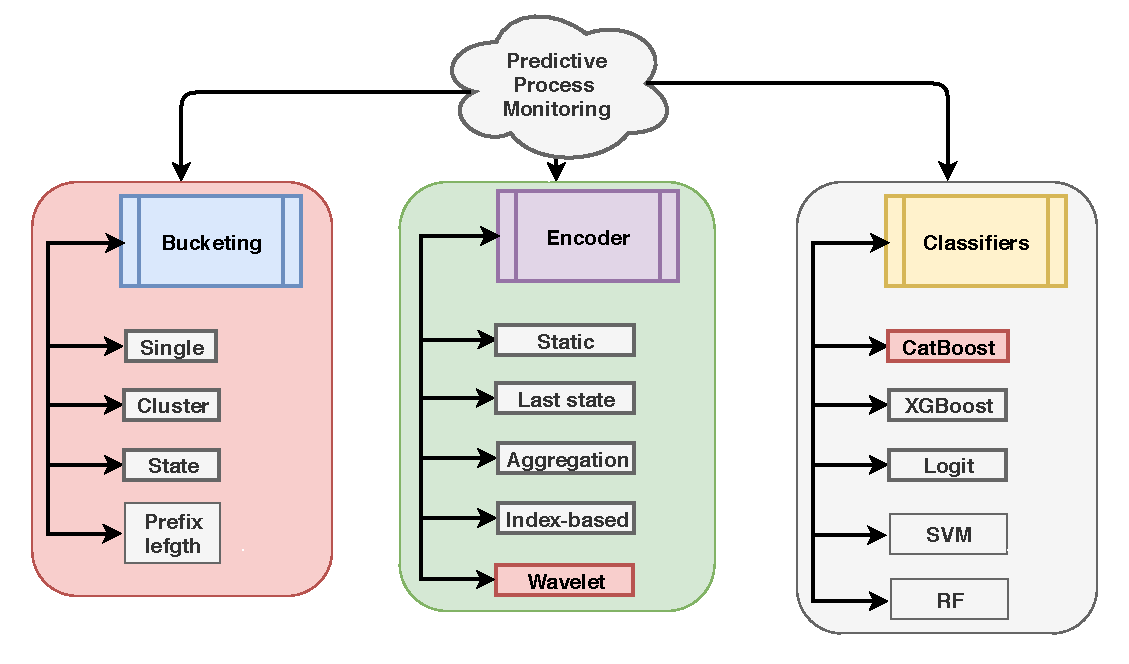
\includegraphics{images/general/all2.pdf}}
		\caption[Predictive process monitoring methods]{Existing and proposed sequence encoding, trace bucketing, and classification methods for outcome-oriented predictive process monitoring.}
		\label{fig:all2}
	\end{center}
\end{figure}

%Within the rest of this chapter, we begin with presenting the %assessment datasets, then describe the assessment methods and %conclude with presenting the results of the experiments.

Within the rest of this chapter, we begin with presenting the assessment event logs, then specifying the assessment methods and end with showing the outcomes of this analysis.

%: ----------------------- paths to graphics ------------------------

% change according to folder and file names
\ifpdf
    \graphicspath{{X/figures/PNG/}{X/figures/PDF/}{X/figures/}}
\else
    \graphicspath{{X/figures/EPS/}{X/figures/}}
\fi

%: ----------------------- contents from here ------------------------

%\input{4/File1}	
%\input{4/File}

\section{Datasets}
Experiments are derived from $7$ real-life historical event logs that include $4$ diverse application domains: \textit{banking} (event logs \textit{BPIC2012} and \textit{BPIC2017}), \textit{government} (\textit{BPIC2015} and \textit{Traffic fines}), \textit{manufacturing} (\textit{Production}), \textit{healthcare (BPIC2011, Sepsis}. All these datasets are publicly available and accessible from the 4TU Centre for Research Data \cite{4TU}. These logs contain dynamic event features, and static case features with 20 different outcome prediction tasks \cite{teinemaa2019outcome} where the final outcome of the case is defined in different approaches based on the business owner's objectives: \quotes{\textit{bpic2012\_A, bpic2012\_C, bpic2012\_D, bpic2017\_A, bpic2017\_C, bpic2017\_R, bpic2015\_1, bpic2015\_2,  bpic2015\_3, bpic2015\_4, bpic2015\_5, traffic, production, bpic2011\_1, bpic2011\_2, bpic2011\_3, bpic2011\_4, sepsis\_1, sepsis\_2, and sepsis\_3.}} In the coming paragraphs, we explain these logs, with the outcome-oriented predictive task in detail.

Table \ref{tab:t1}. shows some general statistics about the 20 event logs, namely the number of traces, min/mid/avg length of traces, number of case and event attributes, etc. This summarization can help when comparing different outcome-oriented predictive process monitoring methods to each other. The datasets have a wide range of characteristics and originate from many different domains.


\begin{center}


\begin{table}[h]
	\caption{Event logs (Datasets) characteristics}
	\label{tab:t1}
	\centering
	\resizebox{\textwidth}{!}{%
		\begin{tabular}{llllllllllllll}			
			\toprule  &  & min  & med  & max      & \# distinct & \# case  & \# event  & \# case  & \# event \\ 
			dataset & \# cases &  length &  length &length &  activities &  variables & variables &  cat values & cat values\\ \midrule
			bpic2011\_1 & 1140 & 1 & 25.0  & 1814 & 193 & 6 & 14 & 961 & 290 \\
			bpic2011\_2 & 1140 & 1 & 54.5  & 1814 & 251 & 6 & 14 & 994 & 370 \\
			bpic2011\_3 & 1121 & 1 & 21.0  & 1368 & 190 & 6 & 14 & 886 & 283 \\
			bpic2011\_4 & 1140 & 1 & 44.0  & 1432 & 231 & 6 & 14 & 993 & 338 \\
			bpic2015\_1 & 694 & 2 & 42.5  & 101 & 380 & 17 & 12 & 17 & 432 \\
			bpic2015\_2 & 753 & 1 & 55.0  & 132 & 396 & 17 & 12 & 7 & 429 \\
			bpic2015\_3 & 1325 & 3 & 42.0  & 124 & 380 & 18 & 12 & 17 & 428 \\
			bpic2015\_4 & 577 & 1 & 42.0  & 82 & 319 & 15 & 12 & 9 & 347 \\
			bpic2015\_5 & 1051 & 5 & 50.0  & 134 & 376 & 18 & 12 & 8 & 419 \\
			production & 220 & 1 & 9.0  & 78 & 26 & 3 & 15 & 37 & 79 \\
			sepsis\_1 & 754 & 5 & 14.0  & 185 & 14 & 24 & 13 & 195 & 38 \\
			sepsis\_2 & 782 & 4 & 13.0  & 60 & 15 & 24 & 13 & 200 & 40 \\
			sepsis\_3 & 782 & 4 & 13.0  & 185 & 15 & 24 & 13 & 200 & 40 \\
			bpic2012\_A & 4685 & 15 & 35.0  & 175 & 36 & 1 & 10 & 0 & 98 \\
			bpic2012\_C & 4685 & 15 & 35.0  & 175 & 36 & 1 & 10 & 0 & 99 \\
			bpic2012\_D & 4685 & 15 & 35.0  & 175 & 36 & 1 & 10 & 0 & 98 \\
			bpic2017\_A & 31413 & 10 & 35.0  & 180 & 26 & 3 & 20 & 13 & 194 \\
			bpic2017\_C & 31413 & 10 & 35.0  & 180 & 26 & 3 & 20 & 13 & 194 \\
			bpic2017\_R & 31413 & 10 & 35.0  & 180 & 26 & 3 & 20 & 13 & 194 \\
			traffic & 129597 & 2 & 4.0  & 20 & 10 & 4 & 14 & 53 & 172 \\
			%hospital\_1 & 77525 & 2 & 6.0  & 217 & 18 & 1 & 21 & 23 & 1756 \\
			%hospital\_2 & 77525 & 2 & 6.0  & 217 & 17 & 1 & 21 & 23 & 1755 \\
			\bottomrule			
		\end{tabular}%
	}
\end{table}
\end{center}

\begin{enumerate}
	\item \textit{BPIC 2012 }
	 Is an event log started in the $2012$ Business Process Intelligence Challenge (BPIC) and includes records related to a loan application process in a large financial institution. The process includes three different subprocesses: (\romannumeral 1) process that records the loan application state; (\romannumeral 2) process that records the loan offer; (\romannumeral 3) process that records the application work items. In this thesis, we deal with a process that tracks the state of the offer. The outcome-oriented predictive task in this event log is if the offer is accepted, declined, or cancelled. This event log is split into three datasets, and each one contains a binary label (e.g. declined vs not declined) to consider it as a binary classification problem. 
	
	\item \textit{BPIC 2017 }
	This event log comes from the $2017$ BPIC and includes records related to the loan application process in a Dutch financial institution which is the same as BPIC $2012$. This version of loan application logs is larger and cleaner than BPIC2012. Similarly to the previous log, BPIC 2017 log is split into three datasets, and each one contains a binary label (e.g. accepted vs not accepted) to consider it as a binary classification problem. 
	
	\item \textit{BPIC 2015 }
	This event log records and combines event logs from $5$ Dutch cities w.r.t a building permit application process. It is split into five different logs, one for each city and the outcome that we aim to predict for predictive monitoring is for each trace if an $LTL$ rule \cite{pnueli1977temporal} is violated or fulfilled \cite{di2017clustering, gunther2014xes}.
	
	\item \textit{Traffic fines }
	This event log records processes related to traffic fines management, and it contains information about fine notification and at the same time, partial repayments. It comes from an Italian police unit. We define the final outcome on the basis of whether the penalty is returned complete or not.
	
	
	
	%This event log records processes related to traffic fines management, and it contains information about fine notification and at the same time, partial repayments. It comes from an Italian police unit. The outcome is based on whether the fina is repaid in full or not. 
	
	\item \textit{Production }
	Is an event log that reports events of the production process. Every case tracks data about the actions, process operators, and resources contributed to items production. We define the final outcome of an ongoing case on the basis of the number of discarded product orders is  more significant than $0$ or not.
	
	%This event log reports events of the manufacturing process. Each trace has information about the activities, process workers, and/or resources contributed to items production. The final outcome is based on whether the number of rejected work orders is bigger than zero or not.
	
	\item \textit{BPIC 2011 }
	This event log shows information about the medical history of patents of a Dutch Academic Hospital, and it comes from the first BPIC. The predictive task w.r.t this log is the same as BPIC 2015 that is for each trace if an $LTL$ rule \cite{pnueli1977temporal} is violated or fulfilled.
	
	%This event log shows information about the medical history of patents from the Gynaecology department of a Dutch Academic Hospital and it comes from the first BPIC. The predictive task w.r.t this log is the same as BPIC 2015 that is for each trace if an LTL rule \cite{pnueli1977temporal} is violated or fulfilled.  
	
	\item \textit{Sepsis }
	Is an event log that holds information about sepsis events from a Dutch hospital. Each trace outlines the pathway for a patient within this clinic. This data set is split into three logs based on the outcome for cases, e.g. whether the patient is admitted to an intensive care unit or not.
	
	%This event log includes information about sepsis cases from a Dutch hospital. Each case represents the pathway for a patient through the hospital. This data set is split into three logs based on the outcome for cases e.g. whether the patient is admitted to an intensive care unit or not.

\end{enumerate}

\section{Experimental setup}
%In this part, we present our technique to split the historical event log into a train, test, and evaluation sets along with describing the evaluation measures that we applied to end with optimizing the hyper-parameters of the proposed methods. 

In this section, we present our technique to divide the historical event logs to a train, test, plus evaluation sets onward with describing each evaluation measure that we applied to end with optimizing the hyper-parameters of the proposed methods. 

\subsection{ Data Preprocessing}
Event logs preprocessing is one of the important and essential steps before building any predictive model \cite{kotsiantis2006data}. To achieve the highest possible prediction accuracy; data preprocessing for all logs should be done beforehand. Firstly we filter out incomplete traces as well as traces that have not been ordered from their beginning.  Secondly, timestamp features are parsed from the prior actions in all traces. Thirdly, For categorical features, the number of levels (i.e. distinct values) are calculated and consider only the most frequent values and other infrequent values are marked as other. Finally, event logs are recorded by enterprise systems, and it could be that some missing data exist. This happens because of the reality that some variables are not relevant to a particular action. In this context, we searched for the nearest preceding event in the same trace where the variables were available and used its value instead.

% Finally, event logs are recorded by enterprise systems, and it could be that some missing data exist. This happens due to the fact that some variables are not applicable to a specific event. In this context, we searched for the nearest preceding event in the same trace where the variables were available and used its value instead.

\subsection{Data splits}
The outcome-oriented predictive process monitoring problem follows the same work-flow of any machine learning problem (see Chapter \ref{ch2}). In order to \textit{tune and evaluate} predictive models, we need to split original event logs into three different parts (see figure \ref{fig:all3}), two of them to train and tune predictive models, and the third acts as unseen data for the model to evaluate its power. In other words, we need to teach an algorithm on how to learn enough to predict cases related to the future along with avoiding \textit{under-fitting} (i.e. learning less than enough)  and \textit{over-fitting} (learn more than enough).  To achieve that, we need to split data into training, and testing sets properly.  There are two methods in machine learning to split original data \cite{mitchell1997machine}: (\romannumeral 1) \textit{train-test split}, and (\romannumeral 2) \textit{cross-validation}.

\begin{figure}[htb]
	\begin{center}
		\resizebox{10cm}{!}{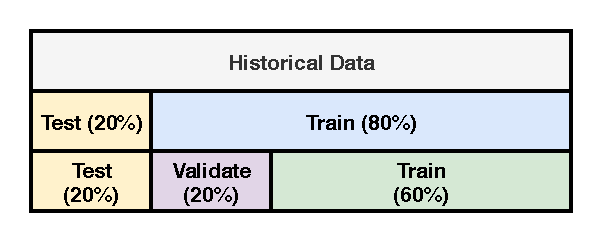
\includegraphics{images/general/all3.pdf}}
		\caption{Data splitting}
		\label{fig:all3}
	\end{center}
\end{figure}

In real life, we train a predictive model on historical data, and apply it to ongoing traces; accordingly, we use \textit{temporal split} (see section \ref{tmp}) to simulate real-life situations. Particularly, business cases are arranged using their timestamps, and the opening $80\%$ is employed for training (i.e. teaching models how to learn from data), and the rest is used to evaluate model performance. In other words, a machine learning classifier is trained and optimized by using all business cases that began before a presented time, and the evaluation  is performed on instances  that begin afterwards. This approach has a drawback which is, the overlapping between events in training cases; accordingly, training cases are cut in a way that events that overlay with evaluation instances are dropped to overcome this problem. 


%This approach has a drawback which is overlapping between events in training cases, and to overcome this problem, training cases are cut in a way that events that overlap with test cases are discarded. 



\subsection{Evaluation Metrics} \label{evm}
As discussed in Chapter \ref{ch2} in section \ref{auc}, a predictive model should be accurate and make a prediction as early as possible, along with predicting a reasonable amount of time. We evaluate the power of the model using three different metrics: accuracy, earliness, and efficiency.

\begin{enumerate}
		\item \textit{Accuracy} AUC has many advantages to use as a measure of the prediction accuracy, (\romannumeral 1) it is unbiased towards a specific class in imbalanced datasets; (\romannumeral 2) It’s a threshold-independent; Accordingly, we used AUC to report model accuracy. To make sure there is no biased viewpoint of results, we reported F-score with the default threshold of $0.5$ as well.
		
		\item \textit{Earliness}. A general strategy to evaluate earliness of forecasts is for each incoming event we calculate the accuracy of prediction based on that event or at fixed time intervals. Meanwhile, the quicker we get the wanted value of accuracy, the more trustworthy the model w.r.t the earliness.
		
		%A general approach to measure earliness of predictions is for each incoming event we calculate the accuracy of prediction based on that event or at fixed time intervals. Meanwhile the earlier we get the desired value of accuracy, the better the model in terms of its earliness. 
		
		\item \textit{Efficiency}. To estimate the execution time for predictive models, we distinguish between the training (or offline) and prediction (or online) phases. In the \textit{training} phase, the total time is calculated based on the total amount of time that is needed for extracting prefixes from the original event log, prefix bucketing, and prefix encoding. When in the \textit{prediction step}, we consider that a forecast is generated virtually immediately since, in real life, forecasts are demanded in real-time. 
		
		 %To measure the execution time for predictive models, we distinguish between the \textit{off-line} and \textit{on-line} phases. In the off-line phase, the total time is calculated based on the total amount of time that is needed for extracting prefix log, bucketing, and encoding prefix traces. When in an on-line step, we consider that a prediction is generated almost immediately as in real life predictions are needed in real-time. In other words, we define on-line time in the meantime for bucketing, and encoding, an incoming event and predicting upon the arrival of this event. 
\end{enumerate}
	


\subsection{Baselines}
We compare our proposed methods against work submitted by \cite{teinemaa2019outcome} as we consider it as a baseline for our work. We used a different combination of existing sequence encoding methods, bucketing types, and classifiers for outcome-oriented predictive process monitoring (see figure \ref{fig:all2}). 

%We will use work proposed by \cite{teinemaa2019outcome} as a baseline to compare our proposed methods

%We compare our proposed methods (see Chapter \ref{ch4}) against work proposed by \cite{teinemaa2019outcome} that we consider it a baseline for our work. 

%several baselines. Firstly, for contributions \ref{catb}, and \ref{dwt}, we used a different combination of existing sequence encoding methods, bucketing types, and classifiers for outcome-oriented predictive process monitoring (see figure \ref{fig:all2}). 

%Secondly, for contribution 3, we compare our approach with the work proposed by \cite{senderovich2019knowledge}. 

We used four different classification algorithms from existing predictive monitoring methods for the experiments and to compare them with the proposed predictive model (i.e. CatBoost): (\romannumeral 1) gradient boosting method (XGBoost) \cite{rozumnyi2017dashboard, senderovich2019knowledge}, random forest (RF) \cite{leontjeva2016complex, cudredata}, support vector machines (SVM), and logistic regression (Logit). For bucketing methods that are based on clustering, we used $k-means$ that is widely used in different domains. 

\begin{table}[0.48\textwidth]
	\caption{Hyper-parameter optimization using TPE}
	\label{tab:t2}
	\begin{tabular}{lllll}
		\hline
		Method                       & Parameter                                                                                                                                                                                                       & Distribution                                                                                                                                      & Values                                                                                                                                                                              &  \\ \hline
		\multicolumn{1}{c}{CatBoost} & \begin{tabular}[c]{@{}l@{}}Learning rate\\ One hot encoding max size\\ Max tree depth\\ Colsample bytree\\ Bagging temperature \\ Scale pos weight\\ L2 leaf regularization\\ number of estimators\end{tabular} & \begin{tabular}[c]{@{}l@{}}uniform\\ uniform integer\\ uniform integer\\ uniform\\ uniform\\ uniform\\ log uniform\\ uniform integer\end{tabular} & \begin{tabular}[c]{@{}l@{}}z $\in$ {[}0.01, 0.8{]}\\ z $\in$ {[}4, 255{]}\\ z $\in$ {[}6, 16{]}\\ z $\in$ {[}0.5, 1{]}\\ z $\in$ {[}0, 100{]}\\ z $\in$ {[}1, 16{]}\\ z $\in$ {[}0, 10{]}\\ z $\in$ {[}500, 1000{]}\end{tabular} &  \\ \hline
		XGBoost                      & \begin{tabular}[c]{@{}l@{}}Learning rate\\ Subsample\\ Max tree depth\\ Colsample bytree\\ Min child weight\\ number of estimators\end{tabular}                                                                 & \begin{tabular}[c]{@{}l@{}}Uniform\\ Uniform\\ Uniform integer\\ Uniform \\ Uniform integer\\ uniform integer\end{tabular}                        & \begin{tabular}[c]{@{}l@{}}z $\in$ {[}0, 1{]}\\ z $\in$ {[}0, 1{]}\\ z $\in$ {[}0, 1{]}\\ z $\in$ {[}0, 1{]}\\ z $\in$ {[}0, 1{]}\\ z $\in$ {[}500, 100{]}\end{tabular}                                                 &  \\ \hline
		RF                           & Max features                                                                                                                                                                                                    & Uniform                                                                                                                                           & z $\in$ {[}0, 1{]}                                                                                                                                                                      &  \\ \hline
		Logit                        & Inverse of regularization strength (C)                                                                                                                                                                          & Uniform integer                                                                                                                                   & $2^z$ , z $\in$ {[}$-$15, 15{]}                                                                                                                                                             &  \\ \hline
		SVM                          & \begin{tabular}[c]{@{}l@{}}Penalty parameter (C)\\ Kernel coefficient (gamma)\end{tabular}                                                                                                    & \begin{tabular}[c]{@{}l@{}}Uniform integer\\ Uniform integer\end{tabular}                                                                         & \begin{tabular}[c]{@{}l@{}}$2^z$ , z $\in$ {[} $-$15, 15{]}\\ $2^z$ , z $\in$ {[}$-$15, 15{]}\end{tabular}                                                                                           
		&  \\ \hline
		K-means                        & Number of clusters                                                                                                                                                                          & Uniform integer                                                                                                                                   & z $\in$ {[}2, 50{]}                                                                                                                                                             &  \\ \hline
	\end{tabular}
	
\end{table}
\restylefloat{table}



\subsection{Hyper-parameter Optimization}
Within each predictive model (or classifier) and clustering algorithms (e.g. k-means)  there are two types of parameters, first type (i.e. \textit{fitted parameters}) that model can learn during the training process, e.g. \textit{weights} of features, and the other type (i.e. \textit{hyper-parameters}) where we need to adjust and tune during the training process to achieve the best possible performance, e.g. \textit{max\_depth, and learning rate}. To tune (or optimize) the hyper-parameter we moreover split the training data to  $60\%$ for training and $20\%$ for tuning (or validation) using \textit{k-fold cross validation} when $k=3$.  The training data is used to train models using combinations of hyper-parameters, where the validation data is applied to evaluate the performance of various hyper-parameter combinations.  We used the $TPE$ algorithm to select the best parameter for our model. Table \ref{tab:t2} shows the bounds and the sampling numbers (i.e. search space) for all of the parameters provided as information to the optimizer.

\begin{figure}[!htbp]
	\begin{center}
		\resizebox{10cm}{!}{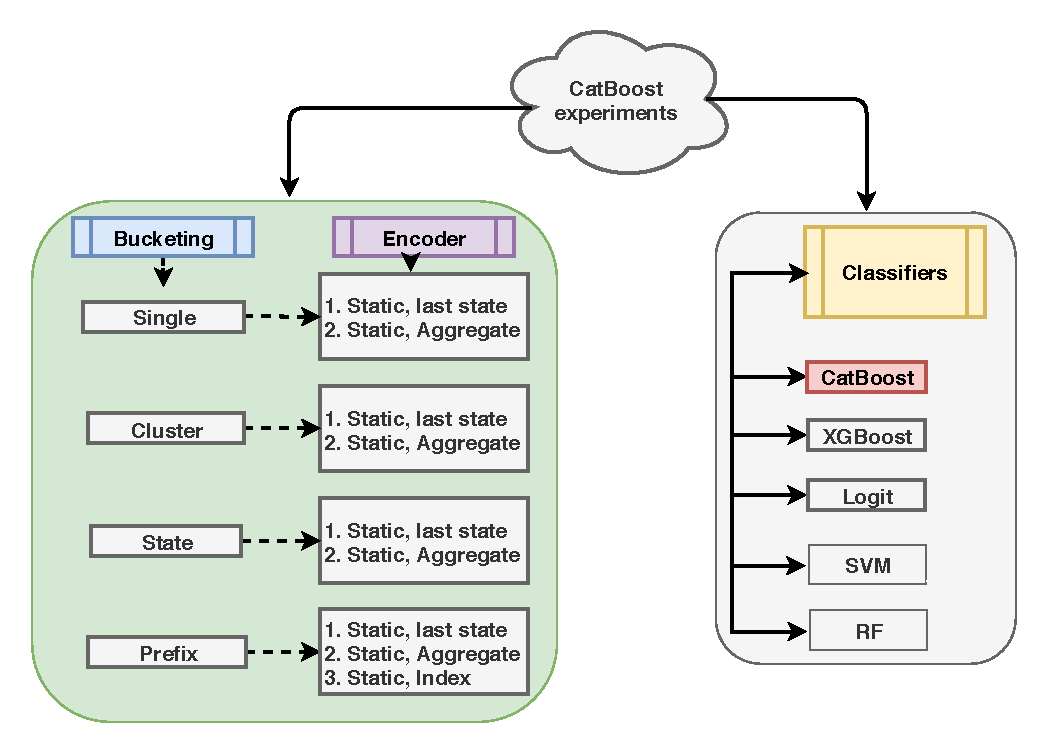
\includegraphics{images/general/dwtnew.pdf}}
		\caption[CatBoost experiments]{Catboost outcome-oriented PPM experiments. }
		\label{fig:cate}
	\end{center}
\end{figure}


\section{Results: accuracy and earliness}
In this section, we provide experiments results in terms of the first two evaluation metrics, i.e. \textit{accuracy and earliness} for our proposed methods to improve the outcome-oriented predictive process monitoring problem.

\subsection{Contribution 1: (CatBoost results)} \label{catresult}
in this part, we executed different experiments based on a different combination between \textit{bucketing, encoding, and classification} methods as shown in figure \ref{fig:cate}








%%%%

% All figures

%%%%%






Overall prediction scores (AUC and F-score) are estimated by calculating the score independently for all prefixes with different length for a given case; after that, we calculate the weighted average of all collected prediction scores.  Weights are corresponding to the number of prefixes employed to calculate the initial prediction scores, and it confirms that scores are controlled fairly by all prefixes, rather than influencing by largest prefixes. Table \ref{tab:t3} show results of CatBoost classifier in terms of AUC and F-score, and for XGBoost, SVM, RF, and Logit results are shown in Tables  \ref{tab:cxgb}, \ref{tab:csvm}, \ref{tab:crf}, and \ref{tab:clogit}. 
% CD Diagram Catboost
\begin{figure}[!htb]
	\begin{center}
		\resizebox{15cm}{!}{\includegraphics{images/catboost/rplot_cd_classifiers.pdf}}
		\caption[Comparison of all classification algorithms using the Nemenyi test]{Critical difference diagram based on the highest AUC values using Nemenyi test shows there is no statistical difference (at $p\-value < \alpha$) between connected methods using a straight line such as CatBoost, XGBoost, and Random Forest.}
		\label{fig:catn}
	\end{center}
\end{figure}


\begin{figure}[!htb]
	\begin{center}
		\resizebox{10cm}{!}{\includegraphics{images/catboost/rplot_cd_catboost.pdf}}
		\caption[Comparison of all bucketing and encoding methods with CatBoost]{
			Critical difference diagram between all trace bucketing and sequence encoding methods shows there is no statistical difference (at $p\-value < \alpha$) between all of them when we use CatBoost classifier.}
		\label{fig:cat3}
	\end{center}
\end{figure}


\begin{figure}[!htb] % "[t!]" placement specifier just for this example
	
	\begin{subfigure}{0.48\textwidth}
		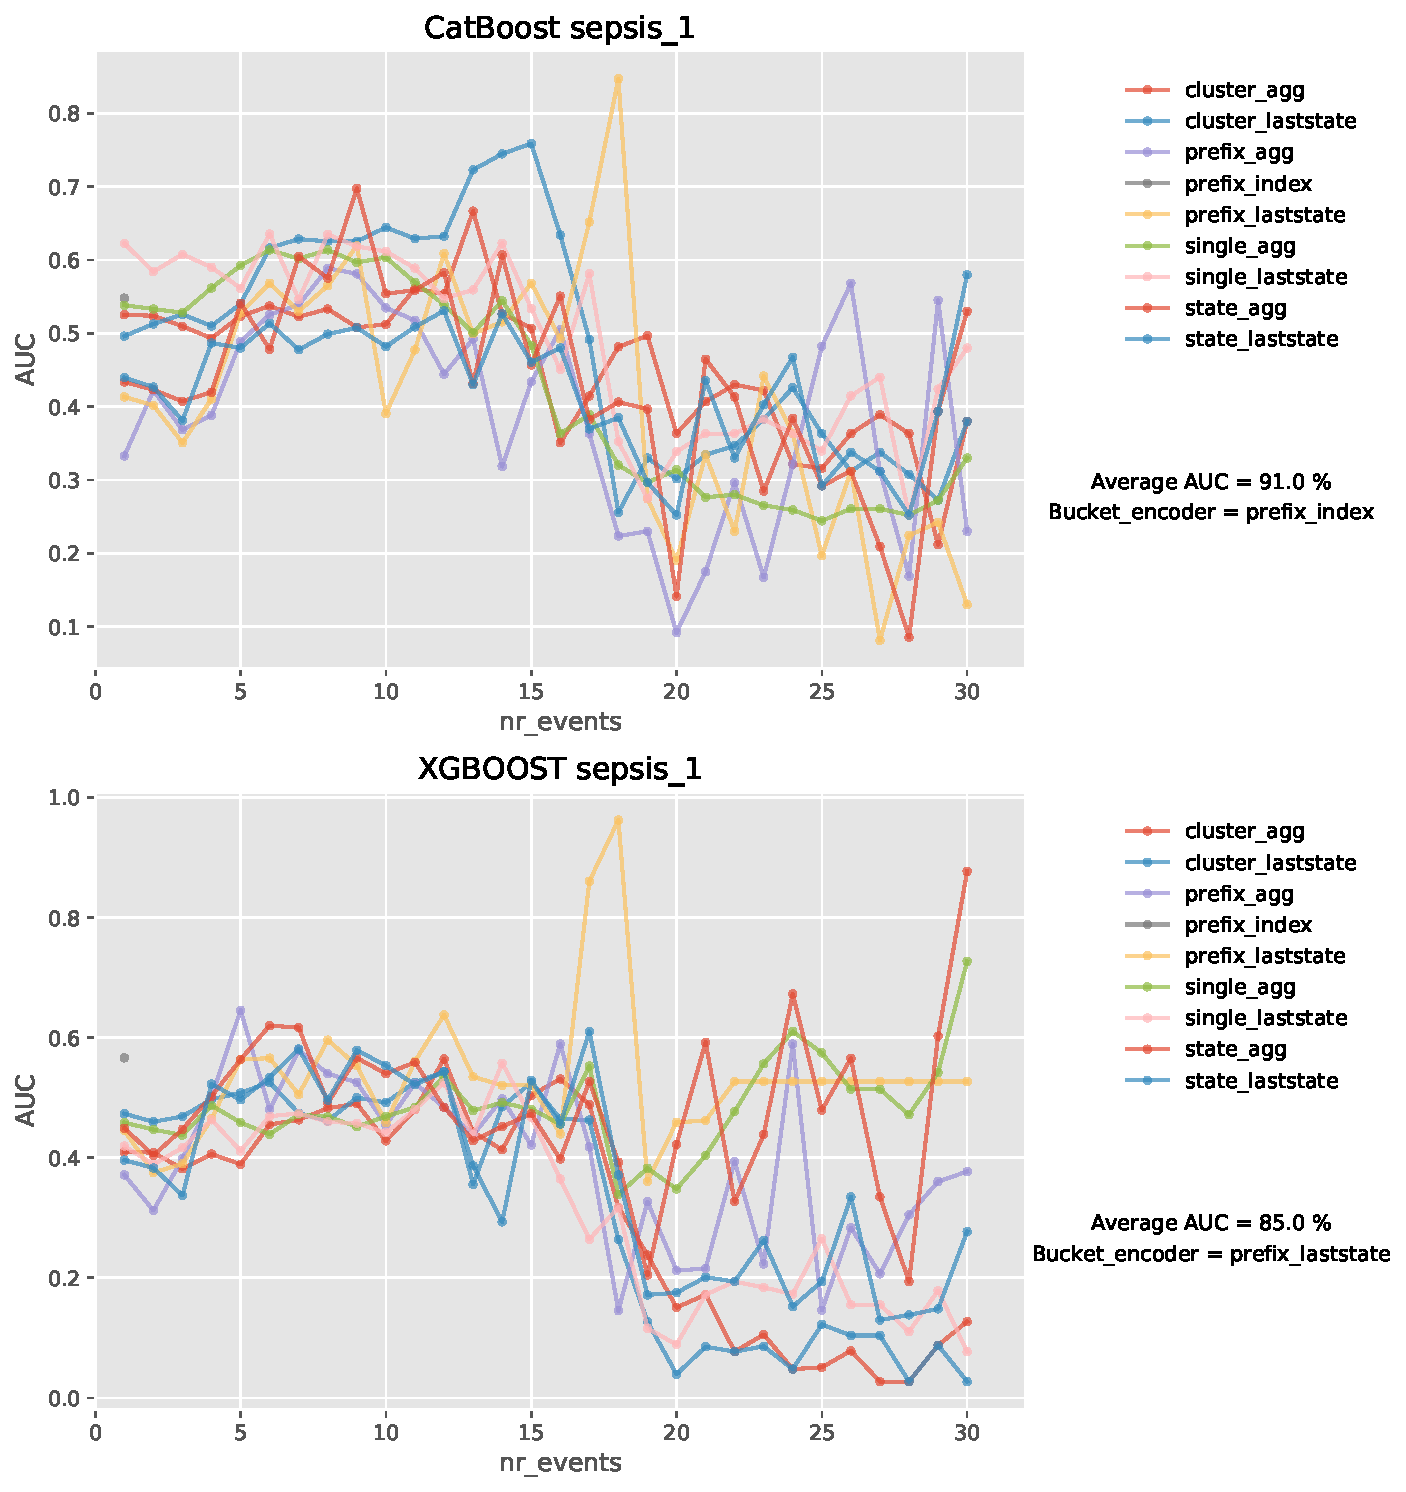
\includegraphics[width=\linewidth]{images/catboost/graphs/sepsis_1_CatBoost_xgboost.pdf}
		\caption{CatBoost vs XGBoost sepsis} \label{fig:sepsis}
	\end{subfigure}\hspace*{\fill}
	\begin{subfigure}{0.48\textwidth}
		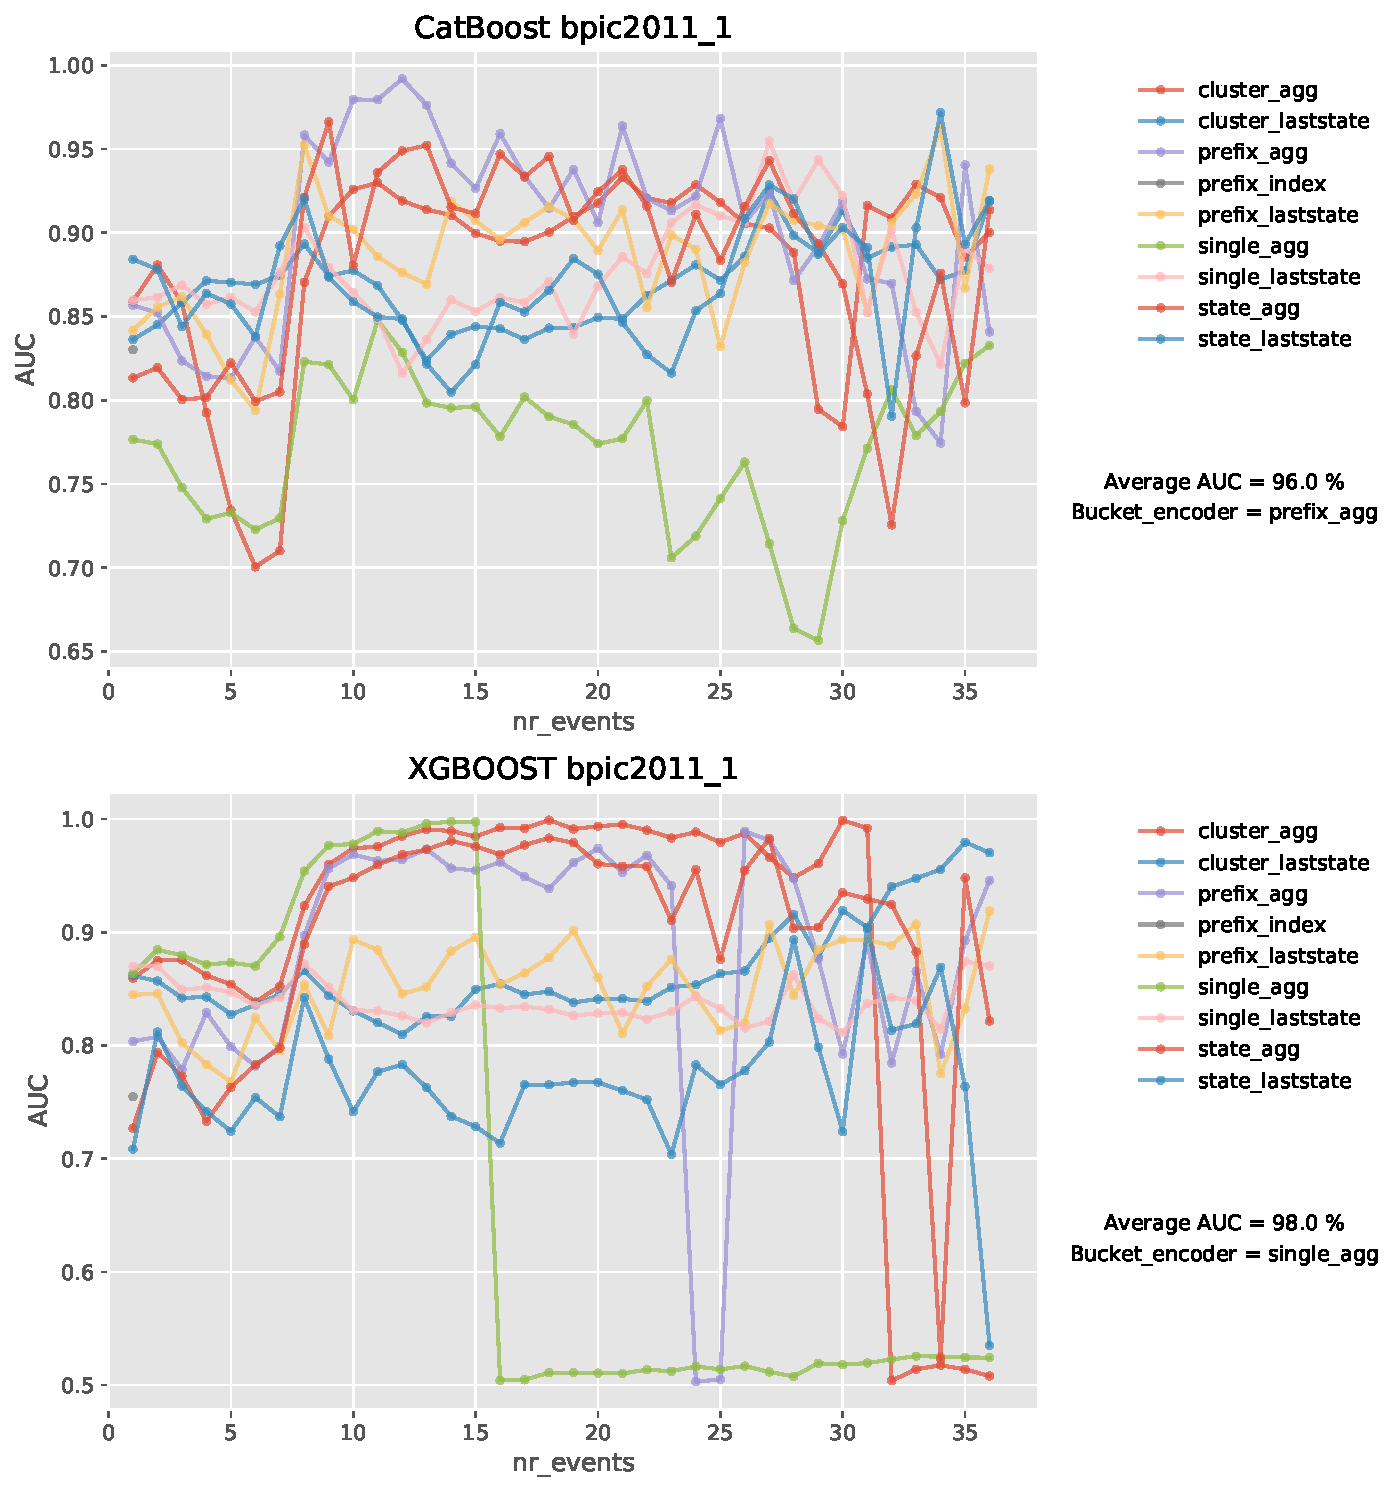
\includegraphics[width=\linewidth]{images/catboost/graphs/bpic2011_1_CatBoost_xgboost.pdf}
		\caption{CatBoost vs XGBoost bpic2011} \label{fig:b11}
	\end{subfigure}
	
	\medskip
	\begin{subfigure}{0.48\textwidth}
		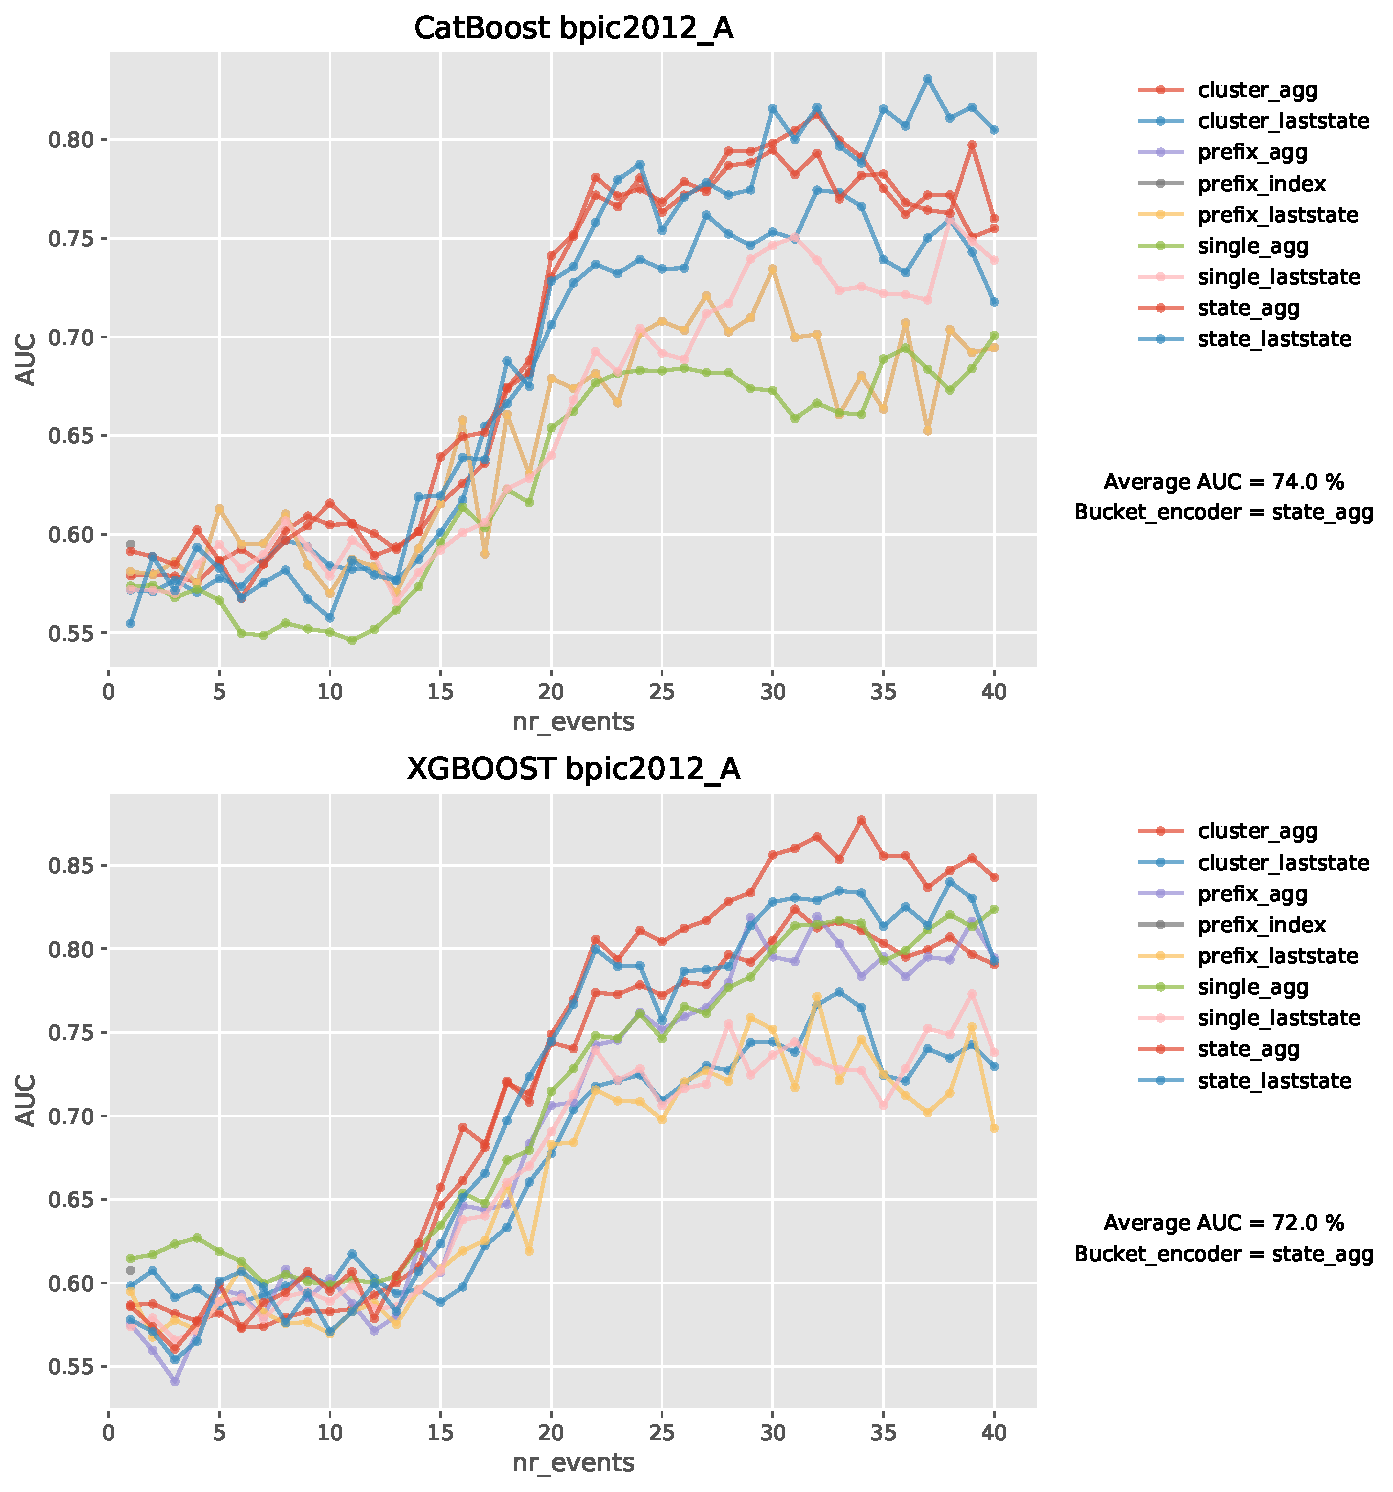
\includegraphics[width=\linewidth]{images/catboost/graphs/bpic2012_A_CatBoost_xgboost.pdf}
		\caption{CatBoost vs XGBoost bpic2012\_A} \label{fig:b12a}
	\end{subfigure}\hspace*{\fill}
	\begin{subfigure}{0.48\textwidth}
		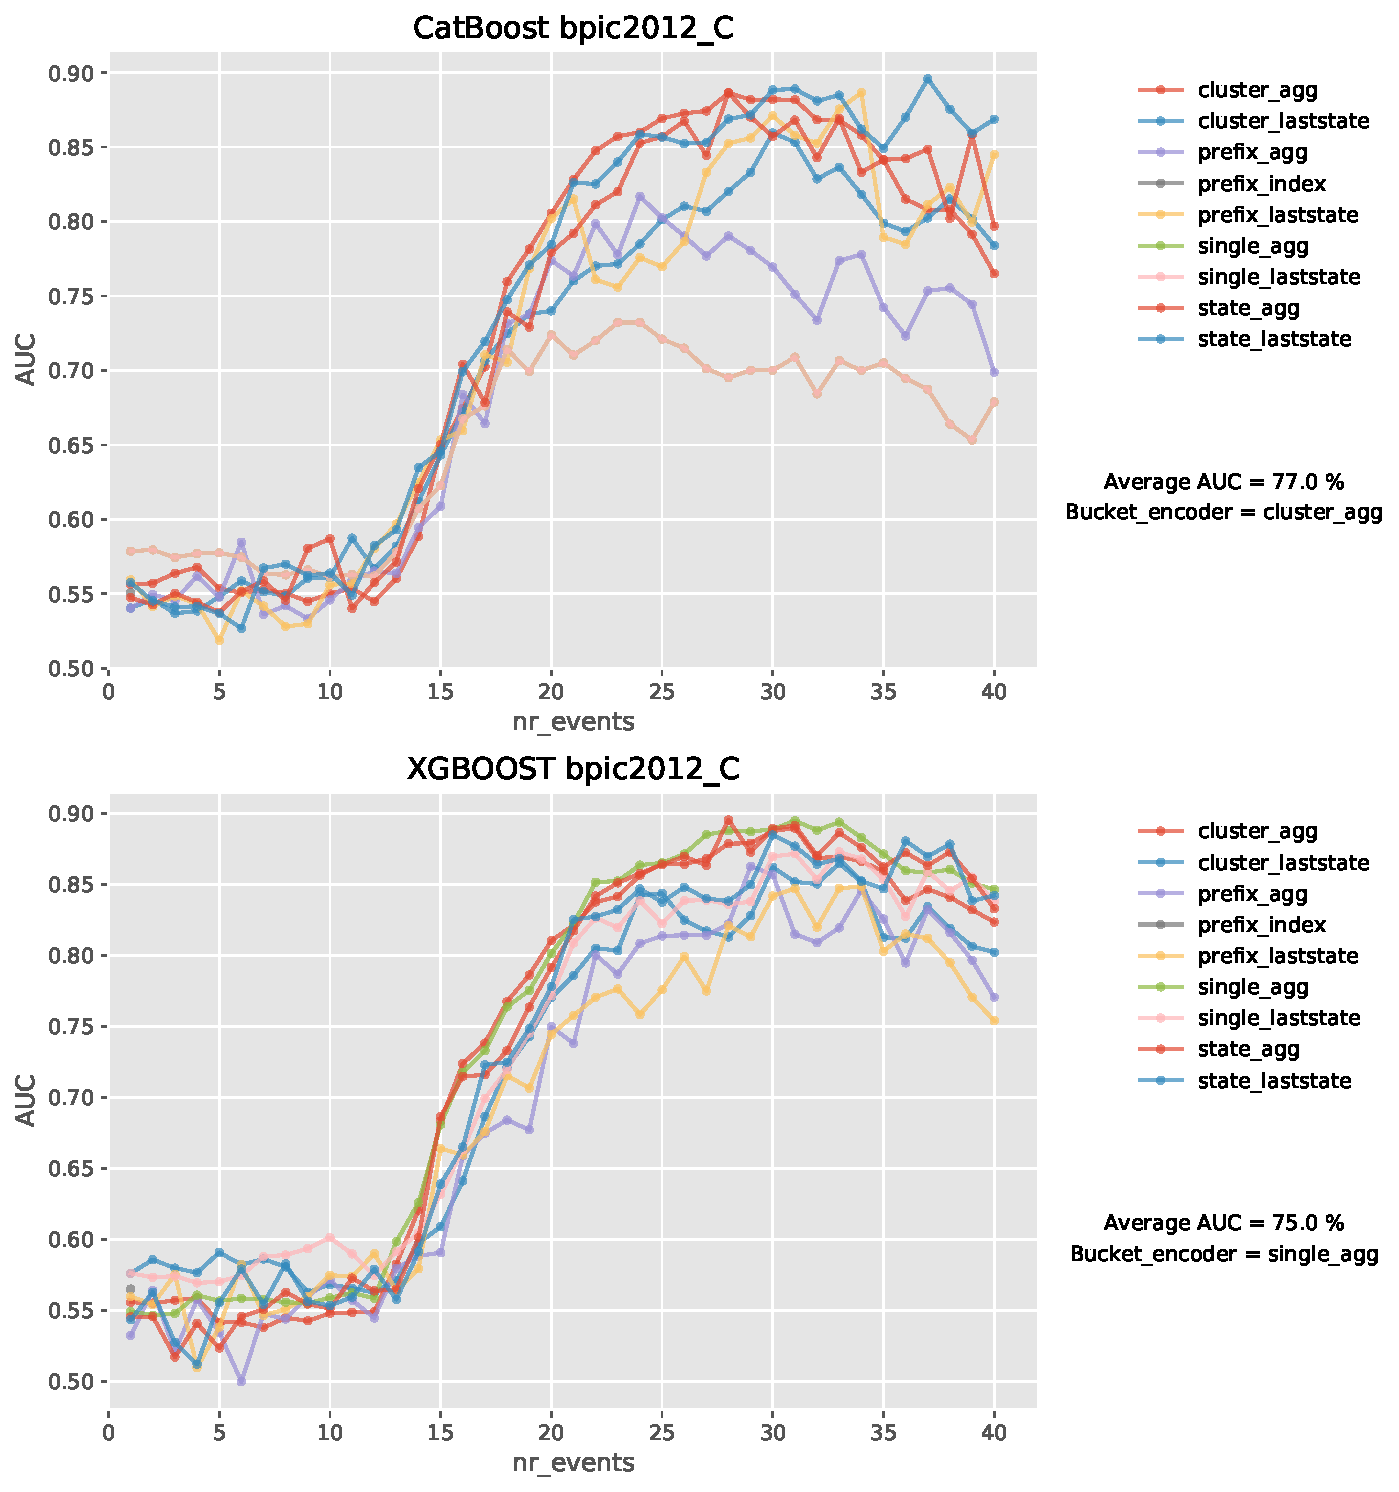
\includegraphics[width=\linewidth]{images/catboost/graphs/bpic2012_C_CatBoost_xgboost.pdf}
		\caption{CatBoost vs XGBoost bpic2012\_C} \label{fig:b12c}
	\end{subfigure}
	\caption{Comparison between CatBoost and XGBoost on all event logs}
\label{fig:r1}
\end{figure}



\begin{figure}[!htb] % "[t!]" placement specifier just for this example
	
	\begin{subfigure}{0.48\textwidth}
		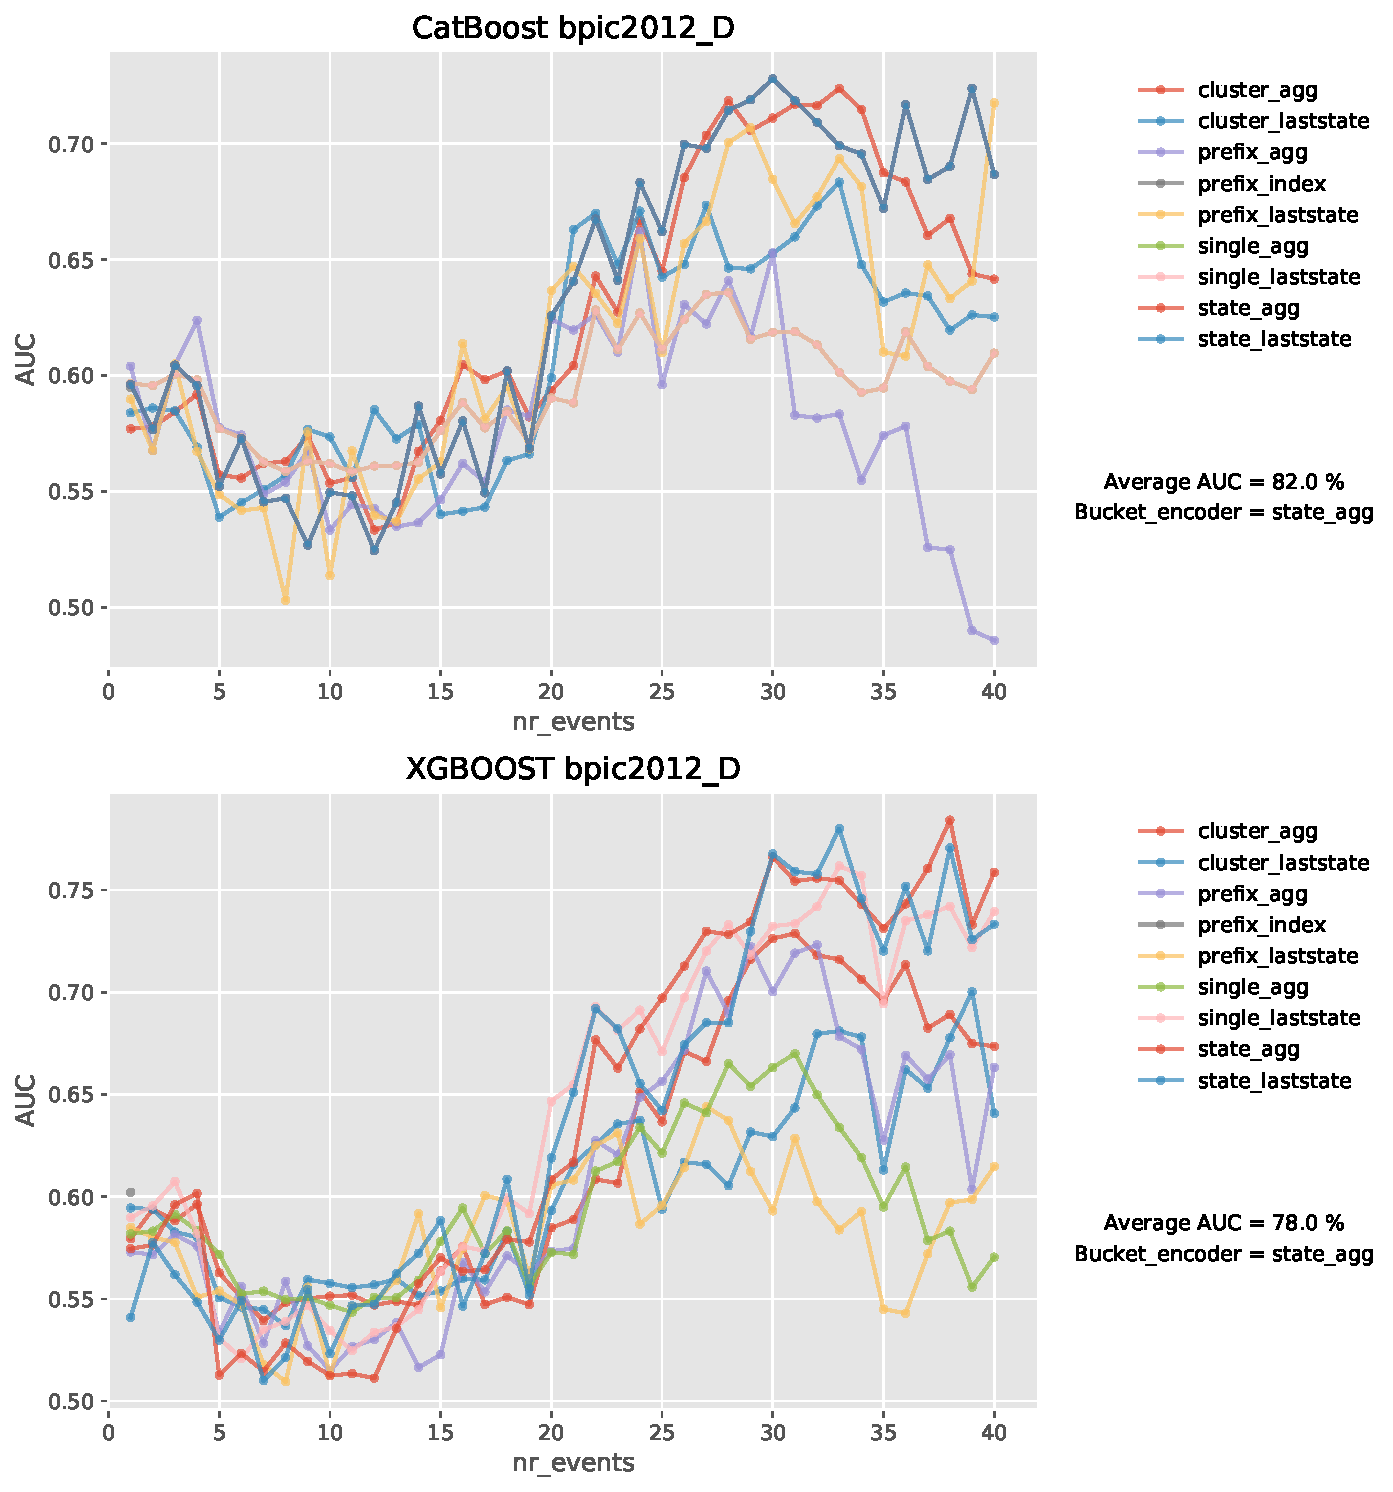
\includegraphics[width=\linewidth]{images/catboost/graphs/bpic2012_D_CatBoost_xgboost.pdf}
		\caption{CatBoost vs XGBoost bpic2012\_D} \label{fig:b12d}
	\end{subfigure}\hspace*{\fill}
	\begin{subfigure}{0.48\textwidth}
		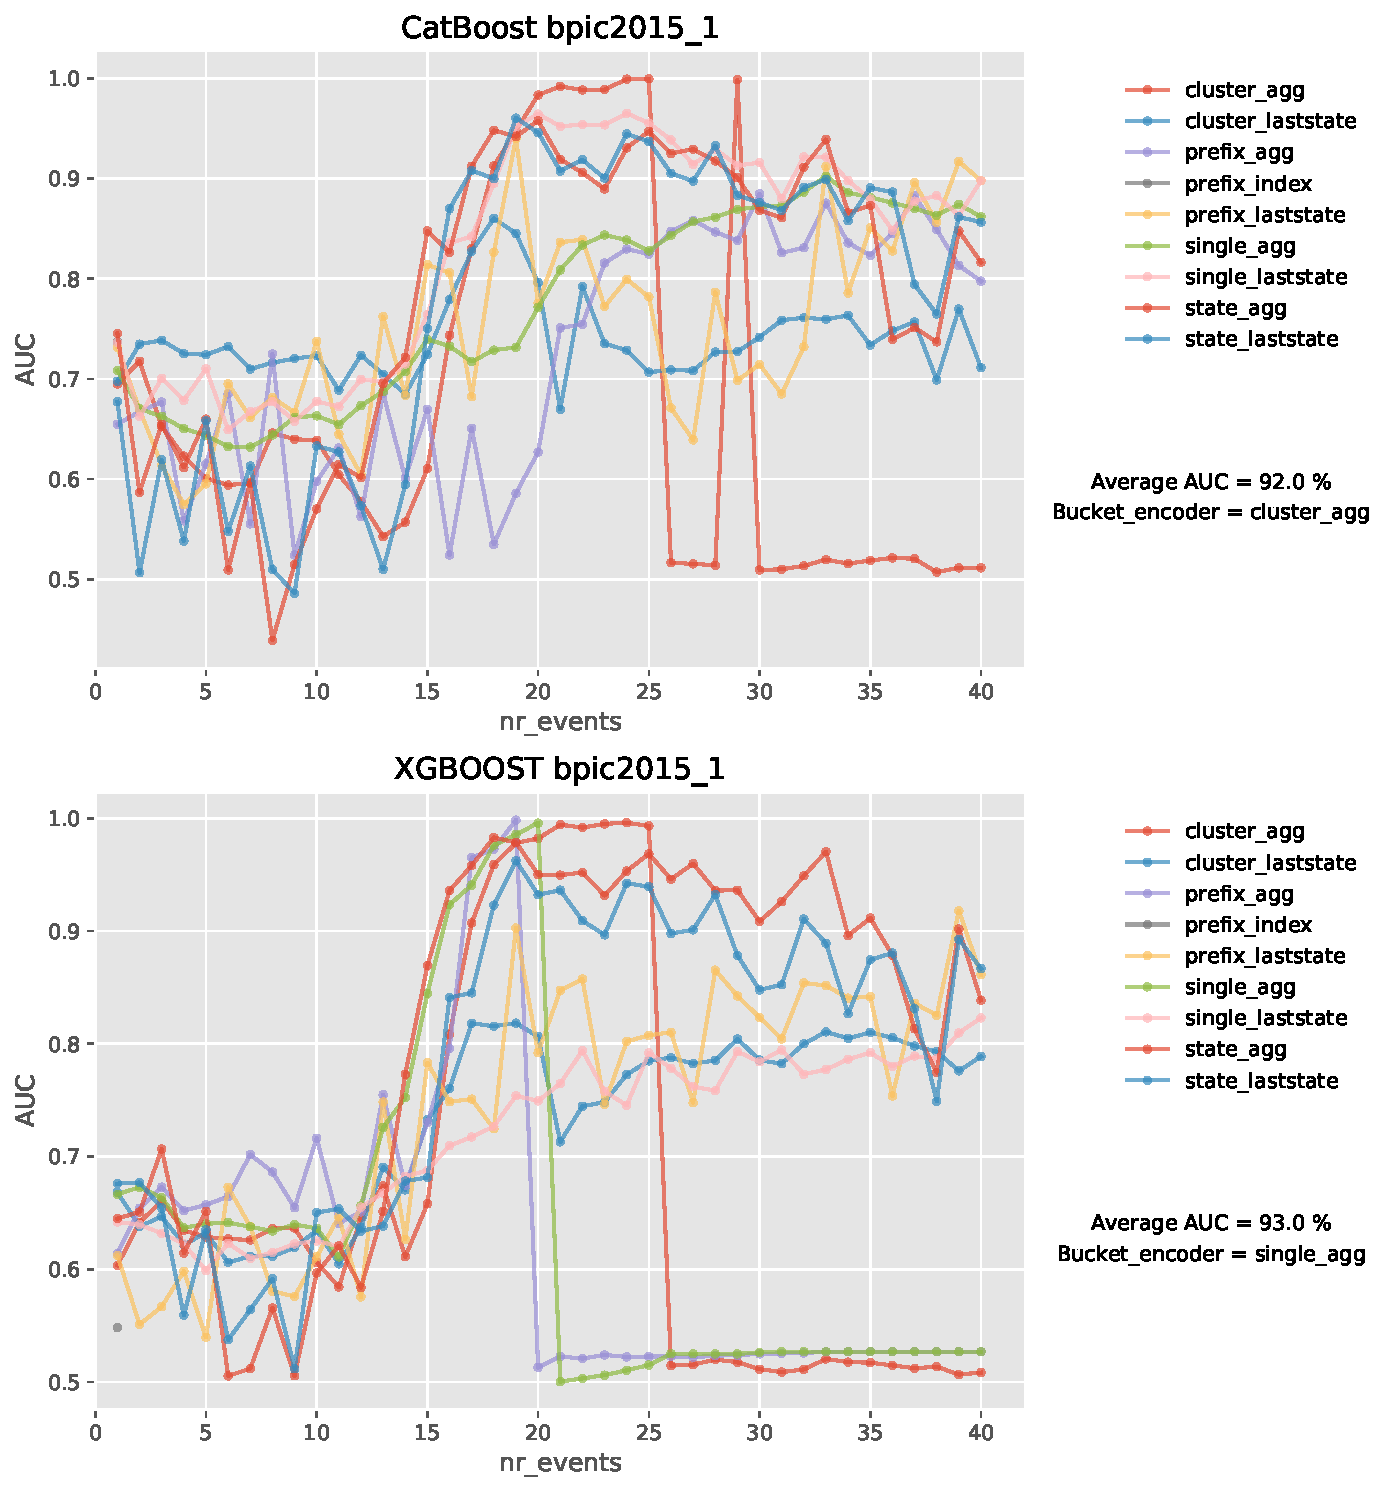
\includegraphics[width=\linewidth]{images/catboost/graphs/bpic2015_1_CatBoost_xgboost.pdf}
		\caption{CatBoost vs XGBoost bpic2015} \label{fig:b151}
	\end{subfigure}
	
	\begin{subfigure}{0.48\textwidth}
		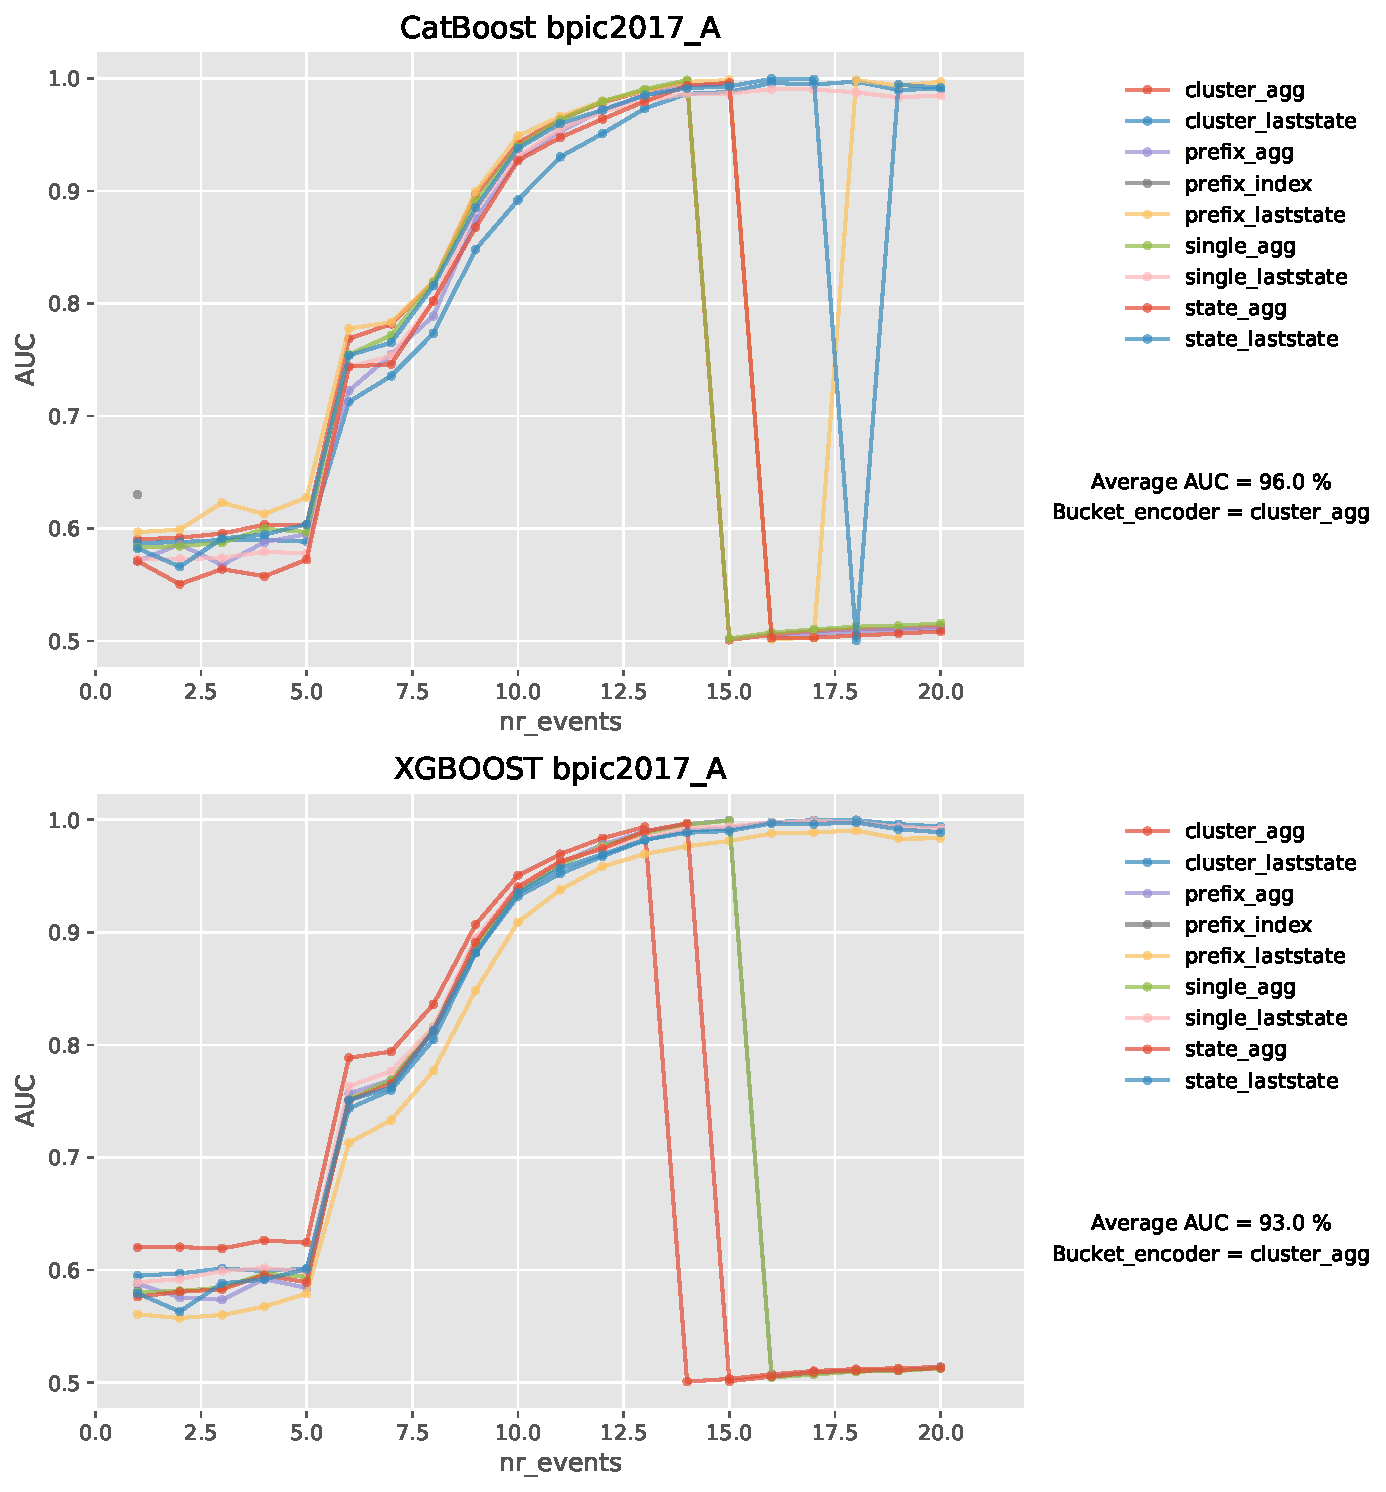
\includegraphics[width=\linewidth]{images/catboost/graphs/bpic2017_A_CatBoost_xgboost.pdf}
		\caption{CatBoost vs XGBoost bpic2017\_A} \label{fig:b17a}
	\end{subfigure}\hspace*{\fill}
	\begin{subfigure}{0.48\textwidth}
		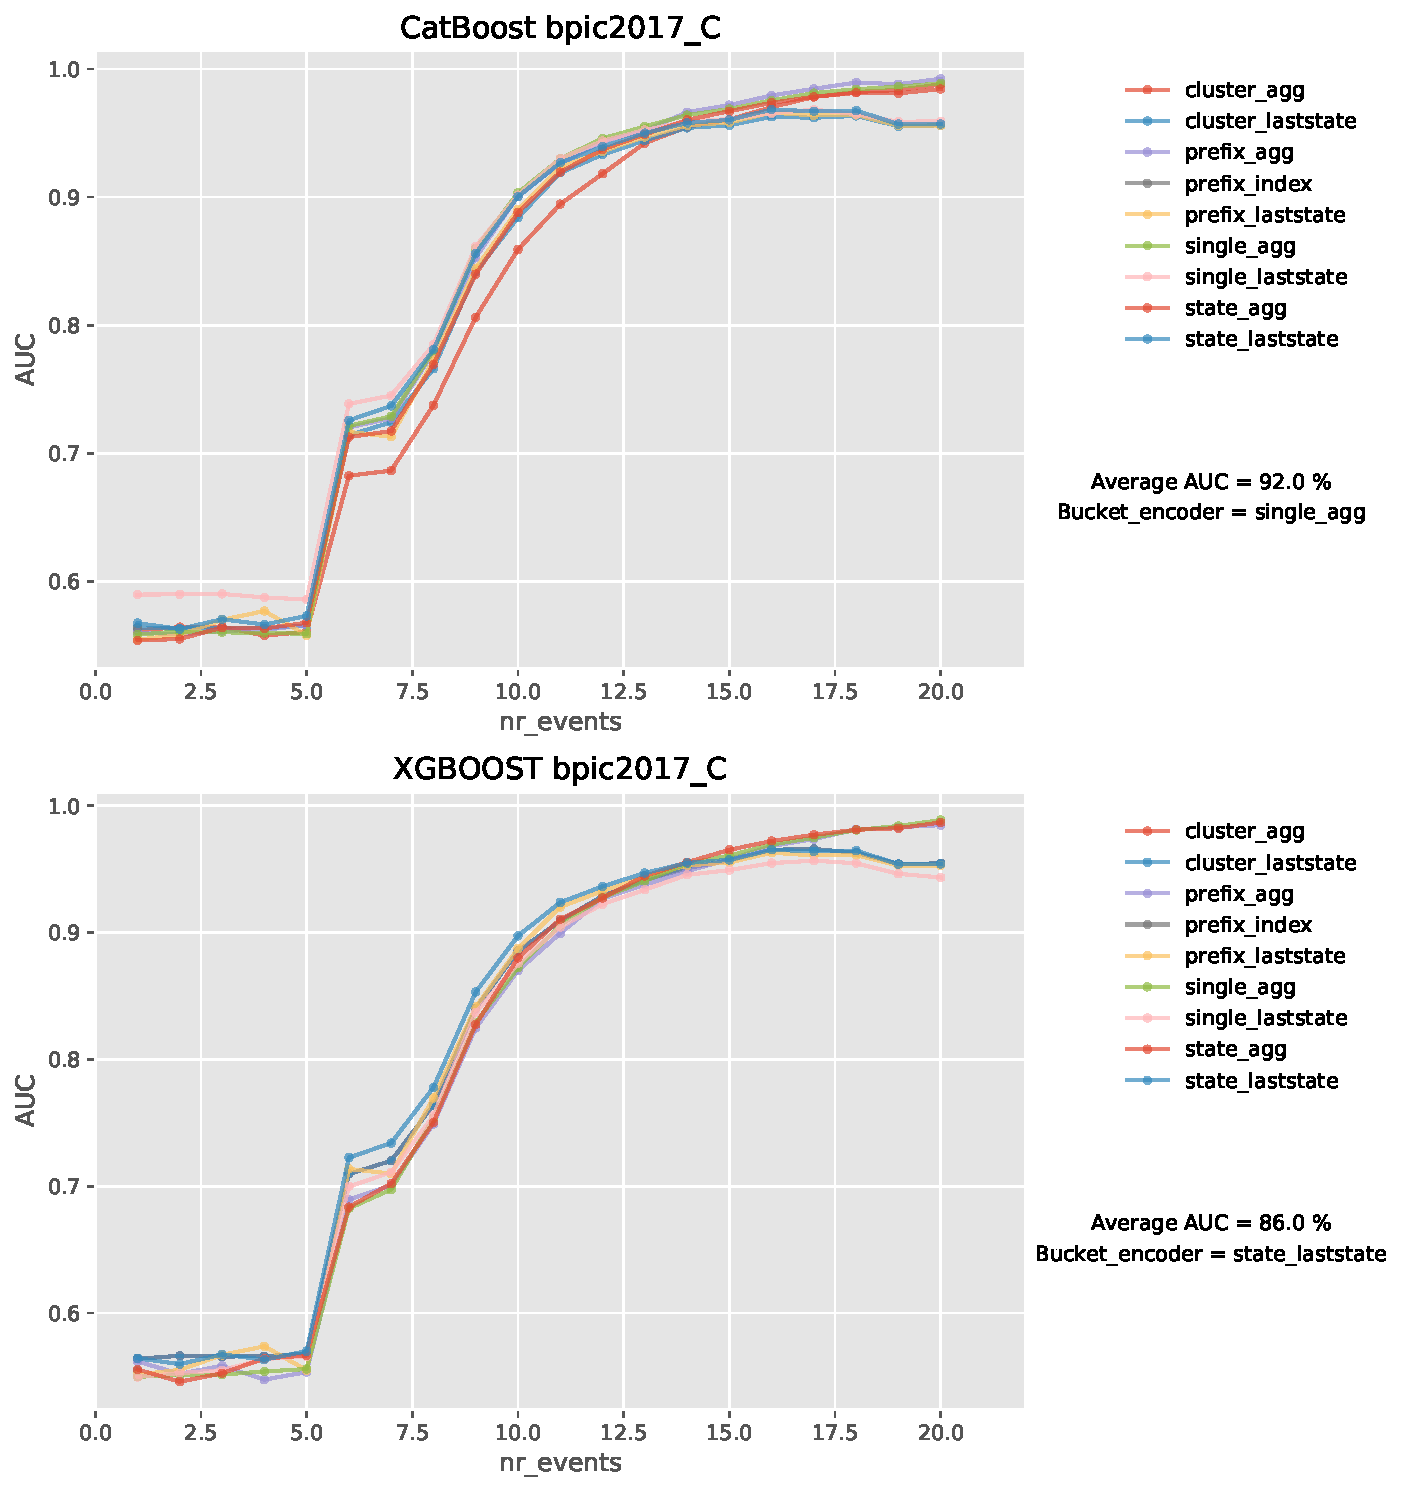
\includegraphics[width=\linewidth]{images/catboost/graphs/bpic2017_C_CatBoost_xgboost.pdf}
		\caption{CatBoost vs XGBoost bpic2017\_C} \label{fig:b17c}
	\end{subfigure}
	\caption{Comparison between CatBoost and XGBoost on all event logs (\textit{continued})}
\label{fig:r2}
\end{figure}


\begin{figure}[!htb] % "[t!]" placement specifier just for this example
	
	\begin{subfigure}{0.48\textwidth}
		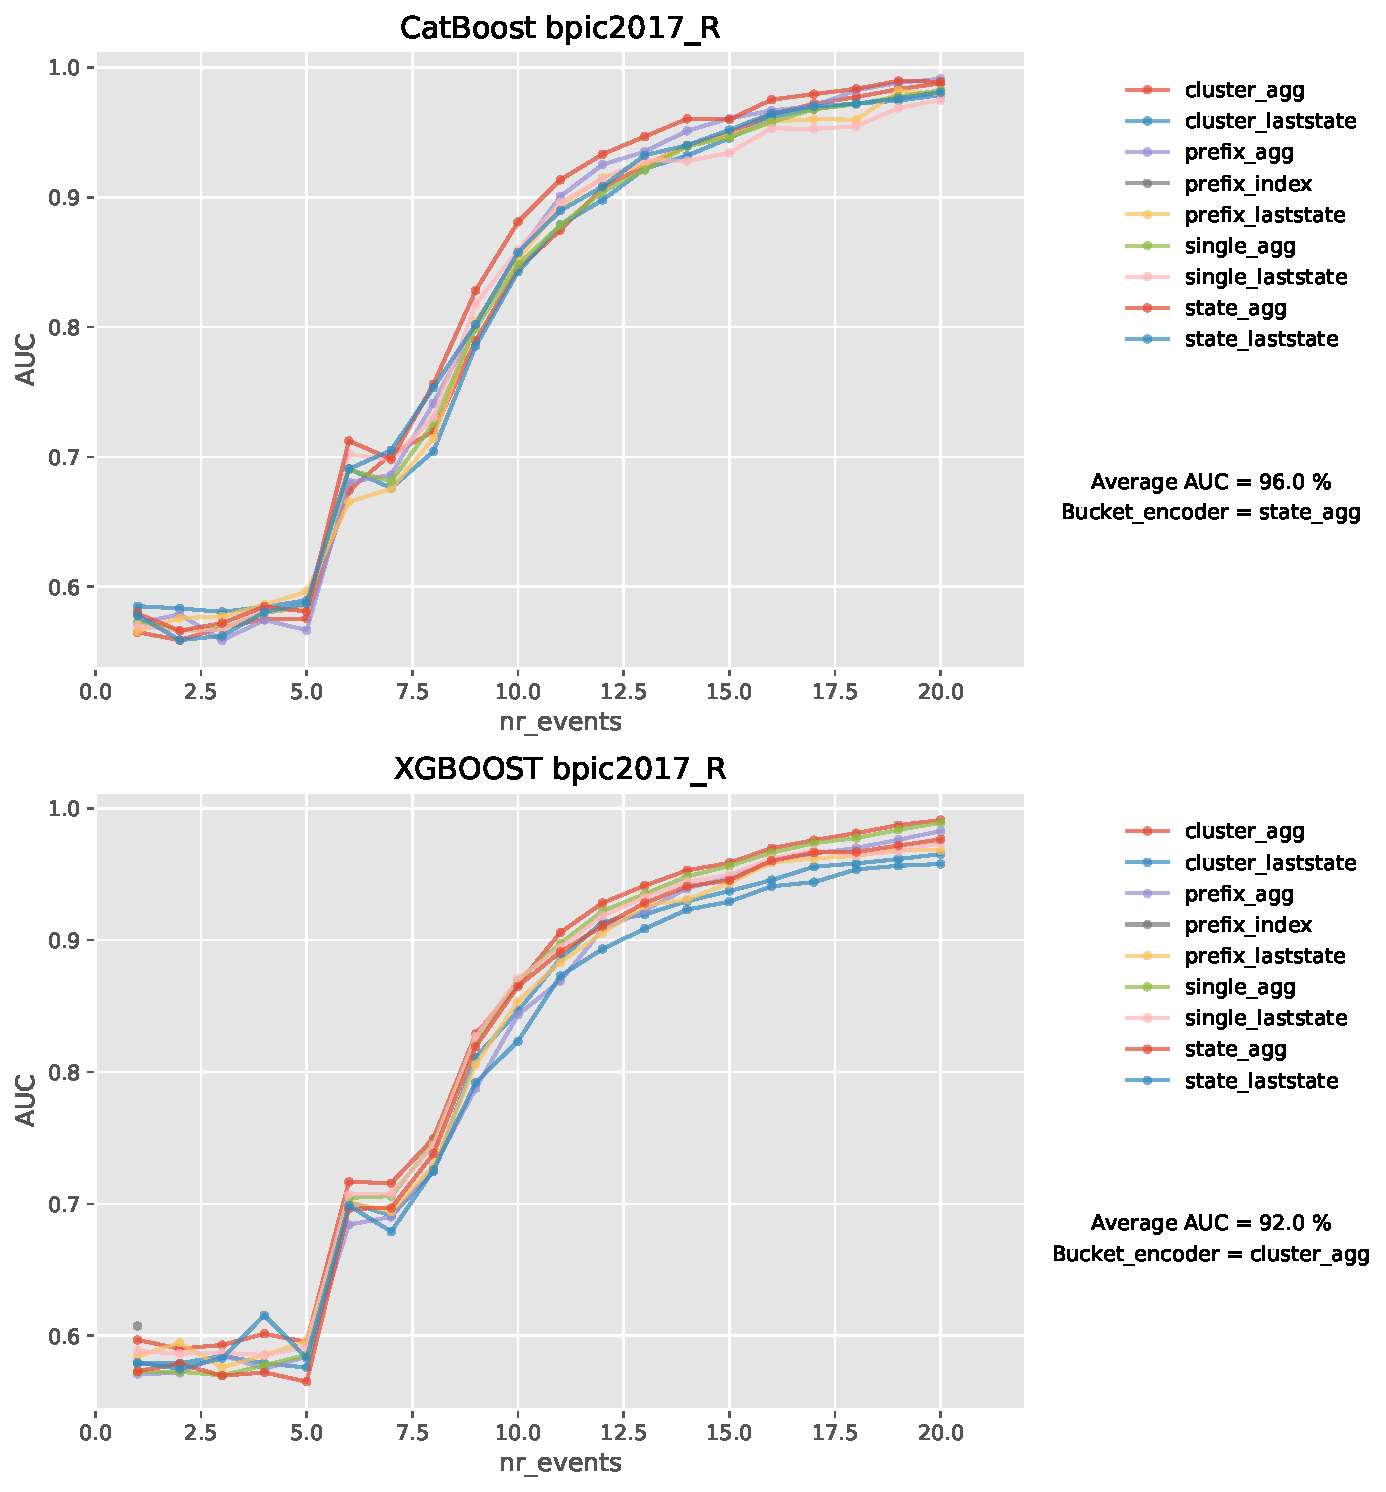
\includegraphics[width=\linewidth]{images/catboost/graphs/bpic2017_R_CatBoost_xgboost.pdf}
		\caption{CatBoost vs XGBoost bpic2017\_R} \label{fig:b17r}
	\end{subfigure}\hspace*{\fill}
	\begin{subfigure}{0.48\textwidth}
		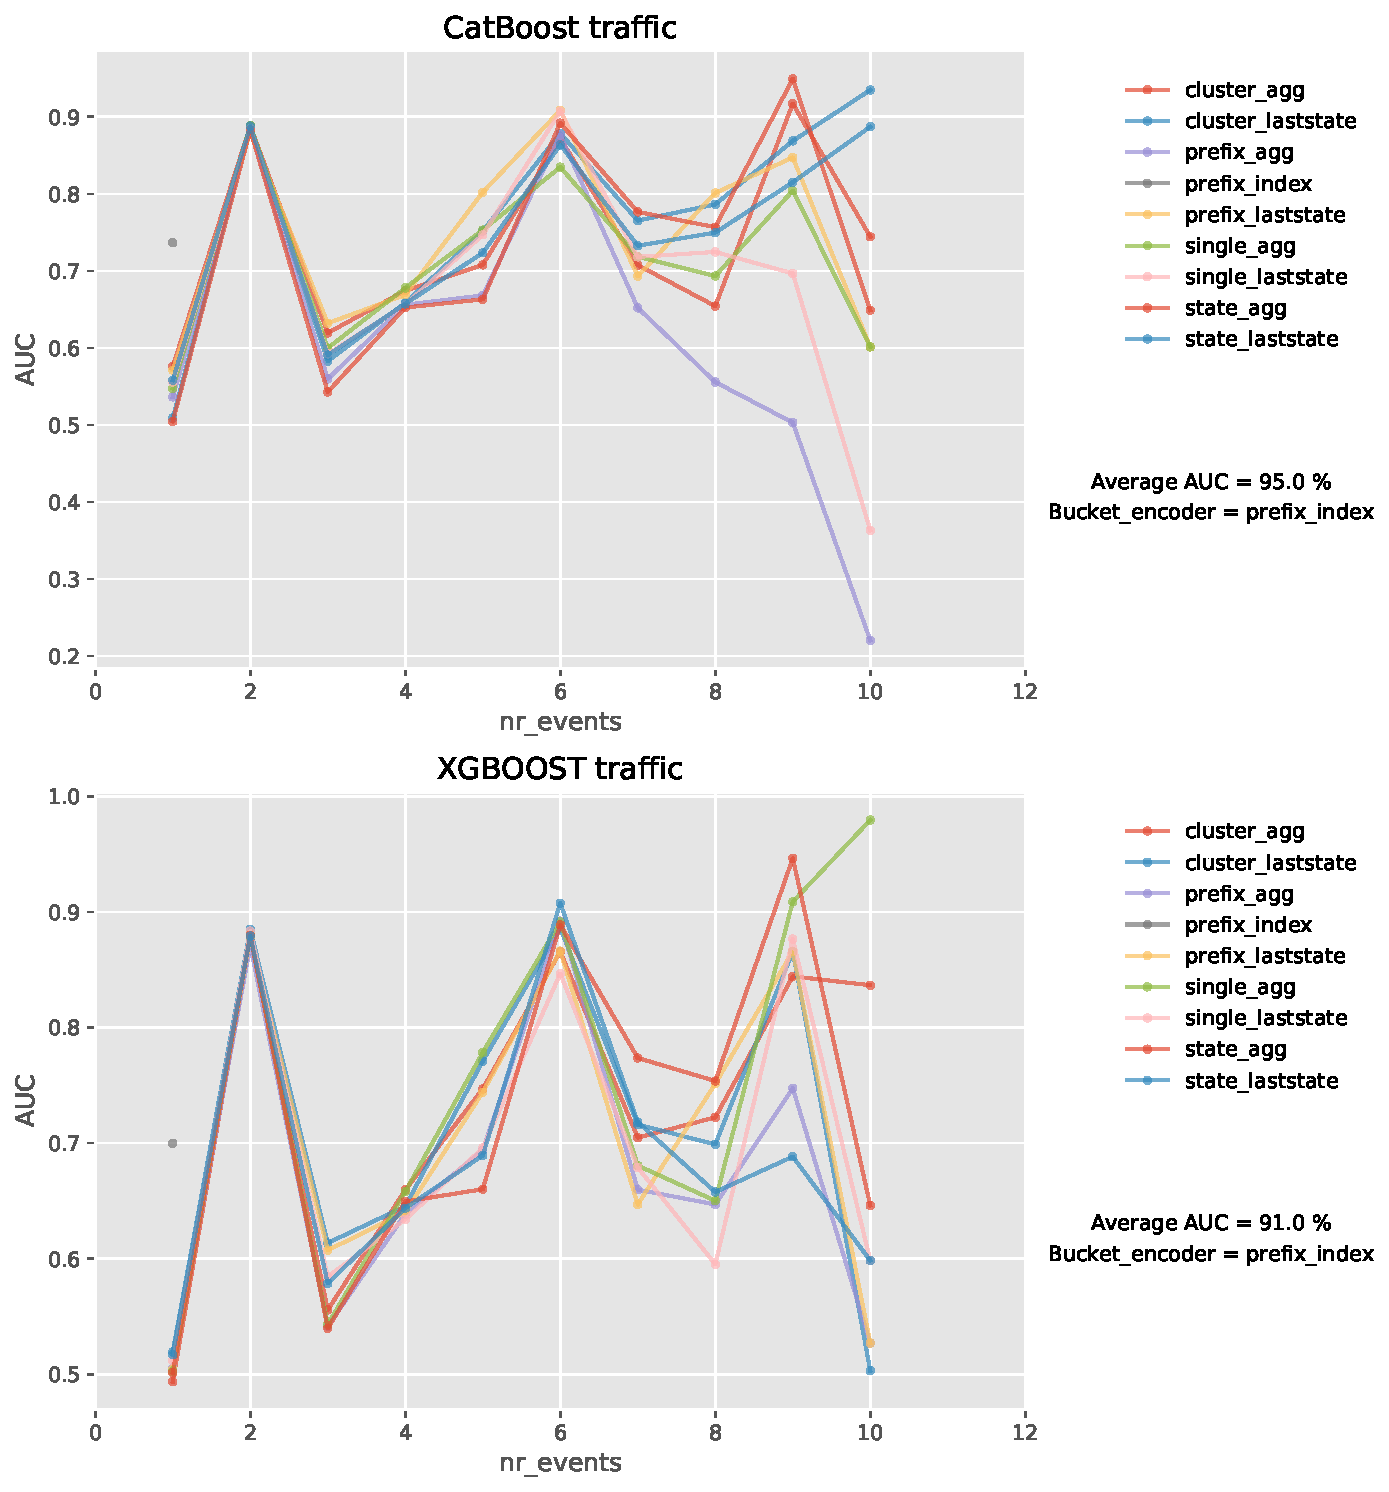
\includegraphics[width=\linewidth]{images/catboost/graphs/traffic_CatBoost_xgboost.pdf}
		\caption{CatBoost vs XGBoost traffic} \label{fig:traf}
	\end{subfigure}
	
	\begin{subfigure}{0.48\textwidth}
		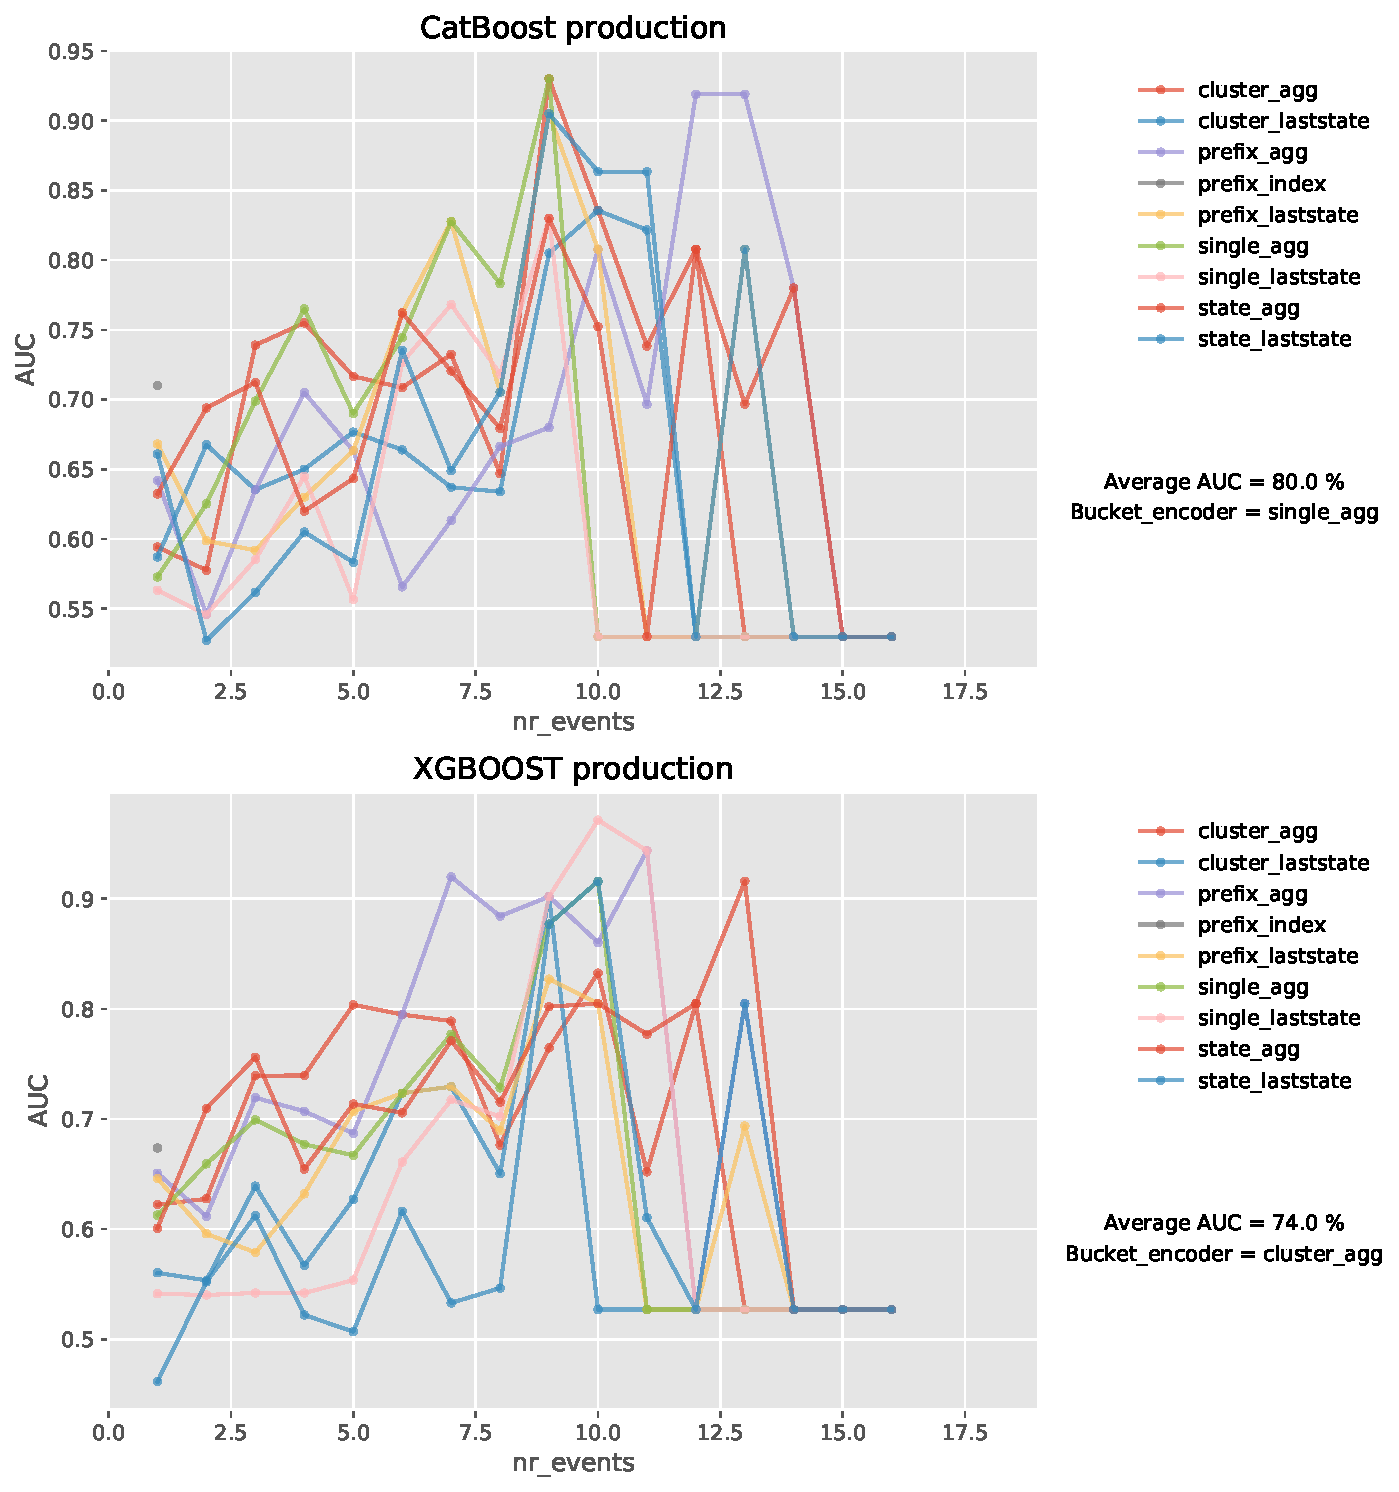
\includegraphics[width=\linewidth]{images/catboost/graphs/production_CatBoost_xgboost.pdf}
		\caption{CatBoost vs XGBoost Production} \label{fig:pro}
	\end{subfigure}\hspace*{\fill}
	\caption{Comparison between CatBoost and XGBoost on all event logs (\textit{continued})}
\label{fig:r3}
\end{figure}


\begin{table}[!htbp]
	\caption{Overall AUC (F-score) for \textbf{CatBoost}}
	\label{tab:t3}
	
	
	\centering
	\resizebox{0.8\textwidth}{!}{%
		\begin{tabular}{llllllll}
			\toprule
			& \multicolumn{5}{c}{catboost}
			\\
			& bpic2012\_a & bpic2011\_4 & bpic2012\_d & bpic2012\_c & production & bpic2015\_4
			\\ \midrule
			single\_agg & $0.62$ ${(0.65)}$ & $\mathbf{0.92}$ $\mathbf{(0.82)}$  & $0.59$ ${(0.19)}$ & $0.64$ ${(0.42)}$ & $0.68$ ${(0.58)}$ & $0.72$ ${(0.14)}$ \\
			state\_laststate & $0.67$ ${(0.68)}$ & $0.86$ ${(0.73)}$ & $\mathbf{0.62}$ $\mathbf{(0.21)}$  & $0.71$ ${(0.5)}$ & $0.64$ ${(0.53)}$ & $0.74$ ${(0.32)}$ \\
			cluster\_laststate & $0.66$ ${(0.64)}$ & $0.9$ ${(0.78)}$ & $0.6$ ${(0.22)}$ & $0.68$ ${(0.46)}$ & $0.65$ ${(0.56)}$ & $0.7$ ${(0.21)}$ \\
			prefix\_laststate & $0.64$ ${(0.66)}$ & $0.91$ ${(0.79)}$ & $0.6$ ${(0.24)}$ & $0.69$ ${(0.43)}$ & $0.67$ ${(0.58)}$ & $0.66$ ${(0.3)}$ \\
			prefix\_agg & $0.64$ ${(0.66)}$ & $0.9$ ${(0.79)}$ & $0.58$ ${(0.17)}$ & $0.67$ ${(0.39)}$ & $0.65$ ${(0.56)}$ & $0.68$ ${(0.28)}$ \\
			state\_agg & $0.68$ ${(0.7)}$ & $0.84$ ${(0.72)}$ & $\mathbf{0.62}$ $\mathbf{(0.21)}$  & $0.7$ ${(0.47)}$ & $0.68$ ${(0.6)}$ & $0.71$ ${(0.19)}$ \\
			cluster\_agg & $0.68$ ${(0.69)}$ & $\mathbf{0.92}$ $\mathbf{(0.79)}$  & $0.61$ ${(0.18)}$ & $0.7$ ${(0.5)}$ & $0.68$ ${(0.59)}$ & $0.65$ ${(0.23)}$ \\
			prefix\_index & $0.59$ ${(0.6)}$ & $\mathbf{0.92}$ $\mathbf{(0.8)}$  & $0.59$ ${(0.6)}$ & $0.55$ ${(0.35)}$ & $0.71$ ${(0.67)}$ & $0.71$ ${(0.26)}$ \\
			single\_laststate & $0.64$ ${(0.69)}$ & $\mathbf{0.92}$ $\mathbf{(0.82)}$  & $0.59$ ${(0.19)}$ & $0.64$ ${(0.42)}$ & $0.61$ ${(0.55)}$ & $0.72$ ${(0.14)}$ \\
			\bottomrule
			\toprule
			& \multicolumn{5}{c}{catboost}
			\\
			& bpic2015\_2 & traffic & sepsis\_3 & sepsis\_2 & bpic2011\_1 & bpic2015\_3
			\\ \midrule
			single\_agg & $0.92$ ${(0.43)}$ & $0.7$ ${(0.74)}$ & $0.74$ ${(0.32)}$ & $0.53$ ${(0.03)}$ & $0.77$ ${(0.69)}$ & $0.66$ ${(0.3)}$ \\
			state\_laststate & $0.89$ ${(0.4)}$ & $0.69$ ${(0.72)}$ & $0.73$ ${(0.37)}$ & $0.36$ ${(0.03)}$ & $0.86$ ${(0.76)}$ & $\mathbf{0.67}$ $\mathbf{(0.32)}$  \\
			cluster\_laststate & $0.76$ ${(0.56)}$ & $0.68$ ${(0.73)}$ & $0.73$ ${(0.32)}$ & $0.53$ ${(0.03)}$ & $0.86$ ${(0.72)}$ & $\mathbf{0.67}$ $\mathbf{(0.3)}$  \\
			prefix\_laststate & $0.95$ ${(0.43)}$ & $0.71$ ${(0.74)}$ & $\mathbf{0.76}$ $\mathbf{(0.36)}$  & $0.53$ ${(0.03)}$ & $0.88$ ${(0.77)}$ & $0.63$ ${(0.24)}$ \\
			prefix\_agg & $0.94$ ${(0.58)}$ & $0.68$ ${(0.69)}$ & $0.72$ ${(0.27)}$ & $0.53$ ${(0.03)}$ & $0.91$ ${(0.76)}$ & $0.61$ ${(0.25)}$ \\
			state\_agg & $0.89$ ${(0.42)}$ & $0.67$ ${(0.67)}$ & $0.73$ ${(0.03)}$ & $0.36$ ${(0.03)}$ & $0.88$ ${(0.75)}$ & $0.64$ ${(0.19)}$ \\
			cluster\_agg & $0.53$ ${(0.98)}$ & $0.71$ ${(0.73)}$ & $0.63$ ${(0.14)}$ & $0.53$ ${(0.03)}$ & $0.88$ ${(0.71)}$ & $0.64$ ${(0.31)}$ \\
			prefix\_index & $0.8$ ${(0.46)}$ & $\mathbf{0.74}$ $\mathbf{(0.21)}$  & $0.73$ ${(0.27)}$ & $0.88$ ${(0.62)}$ & $0.83$ ${(0.77)}$ & $0.6$ ${(0.3)}$ \\
			single\_laststate & $0.86$ ${(0.58)}$ & $0.69$ ${(0.74)}$ & $0.71$ ${(0.27)}$ & $0.53$ ${(0.03)}$ & $0.87$ ${(0.7)}$ & $0.66$ ${(0.3)}$ \\
			\bottomrule
			\toprule
			& \multicolumn{5}{c}{catboost}
			\\
			& bpic2015\_1 & bpic2011\_2 & bpic2011\_3 & bpic2017\_a & bpic2015\_5 & bpic2017\_r
			\\ \midrule
			single\_agg & $0.76$ ${(0.36)}$ & $0.91$ ${(0.84)}$ & $0.95$ ${(0.83)}$ & $0.71$ ${(0.75)}$ & $0.73$ ${(0.53)}$ & $0.8$ ${(0.45)}$ \\
			state\_laststate & $0.77$ ${(0.53)}$ & $0.64$ ${(0.79)}$ & $0.91$ ${(0.8)}$ & $0.82$ ${(0.74)}$ & $0.66$ ${(0.43)}$ & $0.81$ ${(0.49)}$ \\
			cluster\_laststate & $0.74$ ${(0.48)}$ & $0.89$ ${(0.86)}$ & $0.94$ ${(0.81)}$ & $0.83$ ${(0.72)}$ & $\mathbf{0.74}$ $\mathbf{(0.56)}$  & $0.8$ ${(0.48)}$ \\
			prefix\_laststate & $0.74$ ${(0.39)}$ & $0.94$ ${(0.87)}$ & $\mathbf{0.97}$ $\mathbf{(0.87)}$  & $0.81$ ${(0.79)}$ & $0.7$ ${(0.49)}$ & $0.8$ ${(0.49)}$ \\
			prefix\_agg & $0.71$ ${(0.4)}$ & $0.94$ ${(0.86)}$ & $0.95$ ${(0.83)}$ & $0.72$ ${(0.76)}$ & $0.73$ ${(0.51)}$ & $0.81$ ${(0.5)}$ \\
			state\_agg & $0.78$ ${(0.48)}$ & $0.58$ ${(0.77)}$ & $0.91$ ${(0.8)}$ & $0.72$ ${(0.74)}$ & $0.67$ ${(0.52)}$ & $\mathbf{0.82}$ $\mathbf{(0.52)}$  \\
			cluster\_agg & $0.68$ ${(0.6)}$ & $0.52$ ${(0.98)}$ & $0.94$ ${(0.79)}$ & $0.71$ ${(0.8)}$ & $0.73$ ${(0.49)}$ & $0.8$ ${(0.48)}$ \\
			prefix\_index & $0.74$ ${(0.34)}$ & $0.9$ ${(0.89)}$ & $0.96$ ${(0.86)}$ & $0.63$ ${(0.6)}$ & $0.72$ ${(0.16)}$ & $0.58$ ${(0.18)}$ \\
			single\_laststate & $0.82$ ${(0.52)}$ & $0.93$ ${(0.86)}$ & $0.95$ ${(0.85)}$ & $0.84$ ${(0.75)}$ & $0.73$ ${(0.53)}$ & $0.8$ ${(0.46)}$ \\
			\bottomrule
			\toprule
			& \multicolumn{5}{c}{catboost}
			\\
			& bpic2017\_c & sepsis\_1
			\\ \midrule
			single\_agg & $0.82$ ${(0.8)}$ & $0.53$ ${(0.03)}$ \\
			state\_laststate & $0.82$ ${(0.76)}$ & $0.46$ ${(0.11)}$ \\
			cluster\_laststate & $0.81$ ${(0.78)}$ & $\mathbf{0.57}$ $\mathbf{(0.2)}$  \\
			prefix\_laststate & $0.81$ ${(0.75)}$ & $0.48$ ${(0.07)}$ \\
			prefix\_agg & $0.82$ ${(0.79)}$ & $0.45$ ${(0.07)}$ \\
			state\_agg & $0.82$ ${(0.79)}$ & $0.5$ ${(0.15)}$ \\
			cluster\_agg & $0.81$ ${(0.78)}$ & $0.51$ ${(0.1)}$ \\
			prefix\_index & $0.56$ ${(0.62)}$ & $0.55$ ${(0.13)}$ \\
			single\_laststate & $0.83$ ${(0.8)}$ & $0.56$ ${(0.09)}$ \\
			\bottomrule
			
			
		\end{tabular}%
	}
\end{table}

Results show that CatBoost has some improvements against all other classification methods since it gives the best (or shared best) prediction score (i.e. AUC) in $10$ out of $20$ event logs, followed by Xgboost, which shows the best AUC (or shared best) in $5$ event logs, Logit scores the best (or shared best) AUC in $1$ event logs. RF scores the best (or shared best) AUC in $5$ logs. SVM, on average, does not give the equivalent level of scores as the other methods.


We used \textit{A/B testing} to quantify the difference between all classifiers in terms of the performance. We employed the \textit{Nemenyi} test as presented by \cite{demvsar2006statistical}) to plot the \textit{critical difference diagram} as a statistical method to test whether the difference between all methods is significant or not with $\alpha = 0.05$. Critical difference diagram in figure \ref{fig:catn} show that the best performer classifier is CatBoost with an average level of 1.95; however, there is no statistical difference between it, XGBoost, and RF. 



For sequence encoding methods, and trace bucketing, we can see in Table \ref{tab:bsc}  different combinations between them and the number of event logs that each combination worked the best. From these results, we can not say that there is a specific bucketing, and encoding methods worked the best for CatBoost classifier. These results agree with the critical difference diagram, that is shown in figure \ref{fig:cat3}. Figures \ref{fig:r1}, \ref{fig:r2}, and \ref{fig:r3}, show a comparison between the best two classifiers, i.e. CatBoost and XGBoost based on the predicted accuracy in terms of AUC.  All sub-figures contain information about the best AUC and the corresponding bucketing and encoding method while figures \ref{fig:r1cl}, \ref{fig:r1cr}, and \ref{fig:r1cs} in the Appendix show all other comparisons. This analysis gathers the answer to RQ2 (To what extent each of the three methods introduced in Chapter \ref{ch4} enhances the performance of classifiers for PPM, relative to the baseline methods introduced in \cite{teinemaa2019outcome}?), and RQ3 (To what extent is the performance of the three methods introduced in Chapter \ref{ch4} dependent on the choice of classification technique or sequence encoding method?).










%\begin{figure}[htb]
%	%\begin{center}
%	\resizebox{6cm}{!}{\includegraphics{images/wavelet/rplot_cd_all.pdf}}
%	\caption{critical difference diagram for all methods }
%	\label{fig:wavelet4}
%	%\end{center}
%\end{figure}


%\begin{table}[]
%	\caption{Best bucketing and encoding methods across all logs \textbf{Wavelet plus CatBoost}}
%	\label{tab:wavelet1}	
%	\centering
%	\resizebox{0.6\textwidth}{!}{%
	

%\begin{table}[]
	%\caption{Best bucketing and encoding methods across all logs %\textbf{CatBoost}}
	%\label{tab:t4}
	%\centering
	%\resizebox{0.6\textwidth}{!}{%
		
	%
%	}
%\end{table}

                                                         



\clearpage
\subsection{Contribution 2: Complex sequence encoding (Wavelet) results:} \label{wresults}


In this part, we added the complex sequence encoding using discrete wavelet transformation and auto-encoder method that we proposed to the experiments. Now we combine previous encoding methods with the newly added one, as shown in figure \ref{fig:dwt2}. 

We followed the same strategy as we did in section \ref{catresult} where we calculated all prediction scores across all prefix lengths, and after that, we calculated the average score for all predictions based on the number of tested prefixes for each case. 

\begin{figure}[!htb]
	\begin{center}
		\resizebox{10cm}{!}{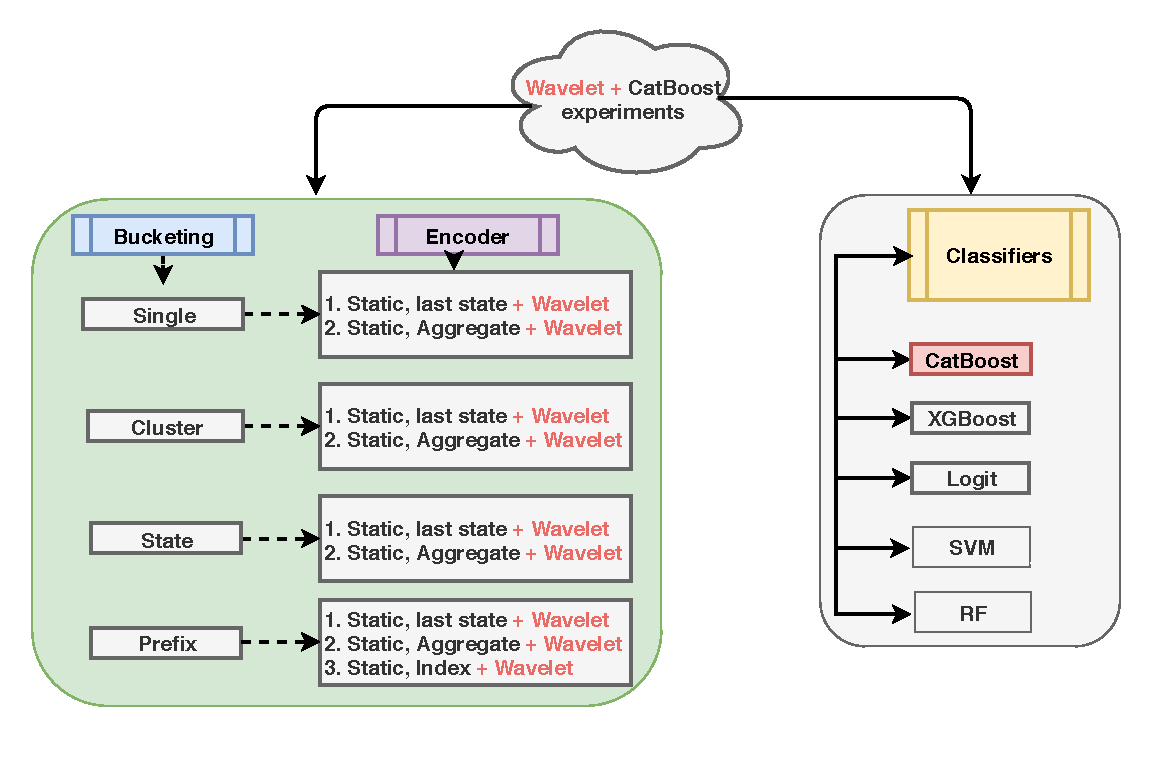
\includegraphics{images/general/catwaveletexp.pdf}}
		\caption{Wavelet plus CatBoost outcome-oriented PPM experiments}
		\label{fig:dwt2}
	\end{center}
\end{figure}


\begin{table}[htb]%\[!htb\]	
	\caption{Bucketing and sequence encoding methods}
	\label{tab:bscwT}
	\begin{subtable}[t]{.5\textwidth}
		\caption{CatBoost}
		\raggedright
		\label{tab:bsc}
		\begin{tabular}{lclll}
			\hline
			\multicolumn{1}{c}{Bucket\_Encoding\_method}                                                                                                                                                                                                                                                                   & \# Data sets                                                              &  &  &  \\ \hline
			\begin{tabular}[c]{@{}l@{}}cluster\_agg\_catboost \\ cluster\_laststate\_catboost  \\ prefix\_agg\_catboost\\ prefix\_index\_catboost\\ prefix\_laststate\_catboost\\ single\_agg\_catboost \\ single\_laststate\_catboost \\ state\_agg\_catboost\\ state\_laststate\_catboost\end{tabular} & \begin{tabular}[c]{@{}c@{}}2\\ 3\\ 2\\ 4\\ 4\\ 1\\ 4\\ 3\\ 3\end{tabular} &  &  &  \\ \hline
		\end{tabular}
	\end{subtable}%
	\begin{subtable}[t]{.5\textwidth}
		\raggedleft
		\caption{Wavelet plus CatBoost}
		\label{tab:bscw}
		\begin{tabular}{lclll}
			\hline
			\multicolumn{1}{c}{Bucket\_Encoding\_Method}                                                                              & \# Data sets                                                              &  &  &  \\ \hline
			\begin{tabular}[c]{@{}l@{}}cluster\_waveletAgg\_catboost\\ cluster\_waveletLast\_catboost\\ prefix\_waveletAgg\_catboost \\ prefix\_WaveletIndex\_catboost\\ prefix\_waveletLast\_catboost\\ single\_waveletAgg\_catboost \\ single\_waveletLast\_catboost\\ state\_waveletAgg\_catboost\\ state\_waveletLast\_catboost\end{tabular} & \begin{tabular}[c]{@{}c@{}}7\\ 2\\ 2\\ 1\\ 2\\ 5\\ 2\\ 5\\ 3\end{tabular} &  &  &  \\ \hline
		\end{tabular}
	\end{subtable}%
\end{table}







Table \ref{tab:catw} show collected results of CatBoost classifier with the wavelet encoding method in terms of AUC and F-score, and for XGBoost, SVM, RF, and Logit results are shown in Tables \ref{tab:wxgba}, \ref{tab:wsvma}, \ref{tab:wrfa}, and \ref{tab:wlogita}.


\begin{table}[!htp]
	\caption{Overall AUC (F-score) for \textbf{Wavelet plus CatBoost}}
	\label{tab:catw}	
	\centering
	\resizebox{0.8\textwidth}{!}{%
		\begin{tabular}{llllllll}
			\toprule
			& \multicolumn{5}{c}{catboost}
			\\
			& bpic2015\_2 & bpic2015\_4 & bpic2012\_c & bpic2011\_4 & bpic2012\_d & traffic
			\\ \midrule
			cluster\_waveletAgg & $0.56$ ${(0.51)}$ & $0.68$ ${(0.26)}$ & $0.73$ ${(0.53)}$ & $\mathbf{0.95}$ $\mathbf{(0.82)}$  & $0.64$ ${(0.21)}$ & $\mathbf{0.74}$ $\mathbf{(0.76)}$  \\
			prefix\_WaveletIndex & $0.79$ ${(0.45)}$ & $0.7$ ${(0.25)}$ & $0.54$ ${(0.34)}$ & $0.91$ ${(0.79)}$ & $0.58$ ${(0.59)}$ & $0.73$ ${(0.2)}$ \\
			prefix\_waveletLast & $0.95$ ${(0.43)}$ & $0.66$ ${(0.3)}$ & $0.69$ ${(0.43)}$ & $0.91$ ${(0.79)}$ & $0.6$ ${(0.24)}$ & $0.71$ ${(0.74)}$ \\
			state\_waveletAgg & $0.92$ ${(0.45)}$ & $0.74$ ${(0.22)}$ & $0.73$ ${(0.5)}$ & $0.87$ ${(0.75)}$ & $\mathbf{0.65}$ $\mathbf{(0.24)}$  & $0.7$ ${(0.7)}$ \\
			single\_waveletLast & $0.87$ ${(0.59)}$ & $0.73$ ${(0.15)}$ & $0.65$ ${(0.43)}$ & $0.93$ ${(0.83)}$ & $0.6$ ${(0.2)}$ & $0.7$ ${(0.75)}$ \\
			single\_waveletAgg & $0.95$ ${(0.46)}$ & $0.75$ ${(0.17)}$ & $0.67$ ${(0.45)}$ & $\mathbf{0.95}$ $\mathbf{(0.85)}$  & $0.62$ ${(0.22)}$ & $0.73$ ${(0.77)}$ \\
			state\_waveletLast & $0.9$ ${(0.42)}$ & $0.75$ ${(0.33)}$ & $0.72$ ${(0.51)}$ & $0.87$ ${(0.74)}$ & $0.63$ ${(0.22)}$ & $0.7$ ${(0.73)}$ \\
			prefix\_waveletAgg & $0.95$ ${(0.59)}$ & $0.69$ ${(0.29)}$ & $0.68$ ${(0.4)}$ & $0.91$ ${(0.8)}$ & $0.59$ ${(0.18)}$ & $0.69$ ${(0.7)}$ \\
			cluster\_waveletLast & $0.77$ ${(0.57)}$ & $0.71$ ${(0.22)}$ & $0.69$ ${(0.47)}$ & $0.91$ ${(0.79)}$ & $0.61$ ${(0.23)}$ & $0.69$ ${(0.74)}$ \\
			\bottomrule
			\toprule
			& \multicolumn{5}{c}{catboost}
			\\
			& bpic2012\_a & bpic2015\_3 & bpic2011\_3 & bpic2011\_2 & sepsis\_2 & bpic2015\_1
			\\ \midrule
			cluster\_waveletAgg & $0.71$ ${(0.72)}$ & $0.67$ ${(0.34)}$ & $0.97$ ${(0.82)}$ & $0.55$ ${(0.51)}$ & $0.56$ ${(0.06)}$ & $0.62$ ${(0.62)}$ \\
			prefix\_WaveletIndex & $0.58$ ${(0.59)}$ & $0.59$ ${(0.29)}$ & $0.95$ ${(0.85)}$ & $0.89$ ${(0.88)}$ & $0.87$ ${(0.61)}$ & $0.73$ ${(0.33)}$ \\
			prefix\_waveletLast & $0.64$ ${(0.66)}$ & $0.63$ ${(0.24)}$ & $0.97$ ${(0.87)}$ & $0.94$ ${(0.87)}$ & $0.53$ ${(0.03)}$ & $0.74$ ${(0.39)}$ \\
			state\_waveletAgg & $0.71$ ${(0.73)}$ & $0.67$ ${(0.22)}$ & $0.94$ ${(0.83)}$ & $0.61$ ${(0.8)}$ & $0.39$ ${(0.06)}$ & $0.81$ ${(0.51)}$ \\
			single\_waveletLast & $0.65$ ${(0.7)}$ & $0.67$ ${(0.31)}$ & $0.96$ ${(0.86)}$ & $0.94$ ${(0.86)}$ & $0.54$ ${(0.04)}$ & $\mathbf{0.83}$ $\mathbf{(0.53)}$  \\
			single\_waveletAgg & $0.65$ ${(0.68)}$ & $\mathbf{0.69}$ $\mathbf{(0.33)}$  & $\mathbf{0.98}$ $\mathbf{(0.86)}$  & $0.94$ ${(0.87)}$ & $0.56$ ${(0.06)}$ & $0.79$ ${(0.39)}$ \\
			state\_waveletLast & $0.68$ ${(0.69)}$ & $0.68$ ${(0.33)}$ & $0.92$ ${(0.81)}$ & $0.65$ ${(0.8)}$ & $0.37$ ${(0.04)}$ & $0.78$ ${(0.54)}$ \\
			prefix\_waveletAgg & $0.65$ ${(0.67)}$ & $0.62$ ${(0.26)}$ & $0.96$ ${(0.84)}$ & $\mathbf{0.95}$ $\mathbf{(0.87)}$  & $0.54$ ${(0.04)}$ & $0.72$ ${(0.41)}$ \\
			cluster\_waveletLast & $0.67$ ${(0.65)}$ & $0.68$ ${(0.31)}$ & $0.95$ ${(0.82)}$ & $0.9$ ${(0.87)}$ & $0.54$ ${(0.04)}$ & $0.75$ ${(0.49)}$ \\
			\bottomrule
			\toprule
			& \multicolumn{5}{c}{catboost}
			\\
			& bpic2015\_5 & sepsis\_3 & bpic2017\_c & production & bpic2017\_r & sepsis\_1
			\\ \midrule
			cluster\_waveletAgg & $\mathbf{0.76}$ $\mathbf{(0.52)}$  & $0.66$ ${(0.17)}$ & $0.71$ ${(0.81)}$ & $0.71$ ${(0.62)}$ & $0.73$ ${(0.51)}$ & $0.54$ ${(0.13)}$ \\
			prefix\_WaveletIndex & $0.71$ ${(0.15)}$ & $0.72$ ${(0.26)}$ & $0.55$ ${(0.61)}$ & $0.7$ ${(0.66)}$ & $0.57$ ${(0.17)}$ & $0.54$ ${(0.12)}$ \\
			prefix\_waveletLast & $0.7$ ${(0.49)}$ & $0.76$ ${(0.36)}$ & $0.81$ ${(0.75)}$ & $0.67$ ${(0.58)}$ & $0.8$ ${(0.49)}$ & $0.48$ ${(0.07)}$ \\
			state\_waveletAgg & $0.7$ ${(0.55)}$ & $0.76$ ${(0.06)}$ & $0.72$ ${(0.82)}$ & $0.71$ ${(0.63)}$ & $0.73$ ${(0.55)}$ & $0.53$ ${(0.18)}$ \\
			single\_waveletLast & $0.74$ ${(0.54)}$ & $0.72$ ${(0.28)}$ & $\mathbf{0.84}$ $\mathbf{(0.81)}$  & $0.62$ ${(0.56)}$ & $0.81$ ${(0.47)}$ & $0.57$ ${(0.1)}$ \\
			single\_waveletAgg & $\mathbf{0.76}$ $\mathbf{(0.56)}$  & $\mathbf{0.77}$ $\mathbf{(0.35)}$  & $0.73$ ${(0.83)}$ & $0.71$ ${(0.61)}$ & $0.76$ ${(0.48)}$ & $0.56$ ${(0.06)}$ \\
			state\_waveletLast & $0.67$ ${(0.44)}$ & $0.74$ ${(0.38)}$ & $0.83$ ${(0.77)}$ & $0.65$ ${(0.54)}$ & $0.82$ ${(0.5)}$ & $0.47$ ${(0.12)}$ \\
			prefix\_waveletAgg & $0.74$ ${(0.52)}$ & $0.73$ ${(0.28)}$ & $0.81$ ${(0.8)}$ & $0.66$ ${(0.57)}$ & $0.79$ ${(0.51)}$ & $0.46$ ${(0.08)}$ \\
			cluster\_waveletLast & $0.75$ ${(0.57)}$ & $0.74$ ${(0.33)}$ & $0.82$ ${(0.79)}$ & $0.66$ ${(0.57)}$ & $0.81$ ${(0.49)}$ & $\mathbf{0.58}$ $\mathbf{(0.21)}$  \\
			\bottomrule
			\toprule
			& \multicolumn{5}{c}{catboost}
			\\
			& bpic2011\_1 & bpic2017\_a
			\\ \midrule
			cluster\_waveletAgg & $0.91$ ${(0.74)}$ & $0.66$ ${(0.73)}$ \\
			prefix\_WaveletIndex & $0.82$ ${(0.76)}$ & $0.62$ ${(0.59)}$ \\
			prefix\_waveletLast & $0.88$ ${(0.77)}$ & $0.81$ ${(0.79)}$ \\
			state\_waveletAgg & $0.91$ ${(0.78)}$ & $0.67$ ${(0.73)}$ \\
			single\_waveletLast & $0.88$ ${(0.71)}$ & $0.8$ ${(0.76)}$ \\
			single\_waveletAgg & $0.8$ ${(0.72)}$ & $0.66$ ${(0.66)}$ \\
			state\_waveletLast & $0.87$ ${(0.77)}$ & $0.69$ ${(0.75)}$ \\
			prefix\_waveletAgg & $0.9$ ${(0.77)}$ & $0.68$ ${(0.77)}$ \\
			cluster\_waveletLast & $0.87$ ${(0.73)}$ & $0.75$ ${(0.73)}$ \\
			\bottomrule
			
		\end{tabular}%
	}
\end{table}


Results show that CatBoost has no improvements against all other classification methods since it gives the best (or shared best) prediction score (i.e. AUC) in $11$ out of $20$ event logs, followed by Xgboost, which shows the best AUC (or shared best) in $5$ event logs, Logit scores the best (or shared best) AUC in $4$ event logs. RF scores the best (or shared best) AUC in $2$ logs. 



Critical difference diagram in figure \ref{fig:cdw} show that the best performer classifier is CatBoost with an average level of 1.8; however, there is no statistical difference between it, XGBoost, Logit, and RF.


\begin{figure}[!htbp]
	\begin{center}
		\resizebox{15cm}{!}{\includegraphics{images/wavelet/rplot_cd_classifiers.pdf}}
		\caption[Critical difference diagram wavelet plus CatBoost]{Critical difference diagram after adding wavelet encoding method based on the highest AUC values using Nemenyi test shows there is no statistical difference (at $p\-value < \alpha$) between connected methods using a straight line such as CatBoost, XGBoost, Random Forest, and Logistic Regression.}
		\label{fig:cdw}
	\end{center}
\end{figure}

For sequence encoding and trace bucketing methods, we can see in Table \ref{tab:bscw} different combinations between them and the number of event logs that each combination worked the best with CatBoost classifier. From these results, we conclude that the \textit{wavelet aggregate} method is the best across all combinations since it achieves the best score over $7$ event logs. 


\begin{figure}[!htbp]
	\begin{center}
		\resizebox{15cm}{!}{\includegraphics{images/wavelet/rplot_cd_catboost.pdf}}
		\caption[Critical difference diagram for all bucketing and encoding methods Wavelet plus CatBoost]{Critical difference diagram between all bucketing and encoding methods based on the highest AUC values using the Nemenyi test shows there is no statistical difference (at $p\-value < \alpha$) between all methods.}
		\label{fig:wavelet5}
	\end{center}
\end{figure}

%Critical difference diagram in figure \ref{fig:wavelet4} reveal that most of the significant combination is associated with CatBoost classifier. 

To compare our proposed complex sequence encoding method using discrete wavelet transformation and autoencoder, we used all classifiers with all previous encoding methods as a baseline; then we applied wavelet encoder with all classifiers. Figures \ref{fig:r1w}, \ref{fig:r2w}, and \ref{fig:r3w} show the results from the XGBoost classifier before and after applying wavelet encoder, and each subfigure contains the results for a specific event log in addition to the average AUC that associated with the best bucketing and encoding method for the baseline and the proposed method. We conclude from these experiments that using wavelet encoder with other simple encoding methods improved the overall AUC in most of the event logs, however for CatBoost the situation is different since the accuracy is not improved and this could happen because CatBoost classifier works very well with lots of categorical features and using wavelet encoder we decreased the available number of categorical attributes by adding more numeric features to the predictive models. Figures \ref{fig:wc1} (CatBoost), \ref{fig:wl1} (Logit), \ref{fig:wr1} (RF), and \ref{fig:ws1} (SVM) in the Appendix contain the comparison for all classifiers with and without the wavelet method. 

%%%%

% All figures

%%%%%



\begin{figure}[!htbp] % "[t!]" placement specifier just for this example
	
	\begin{subfigure}{0.48\textwidth}
		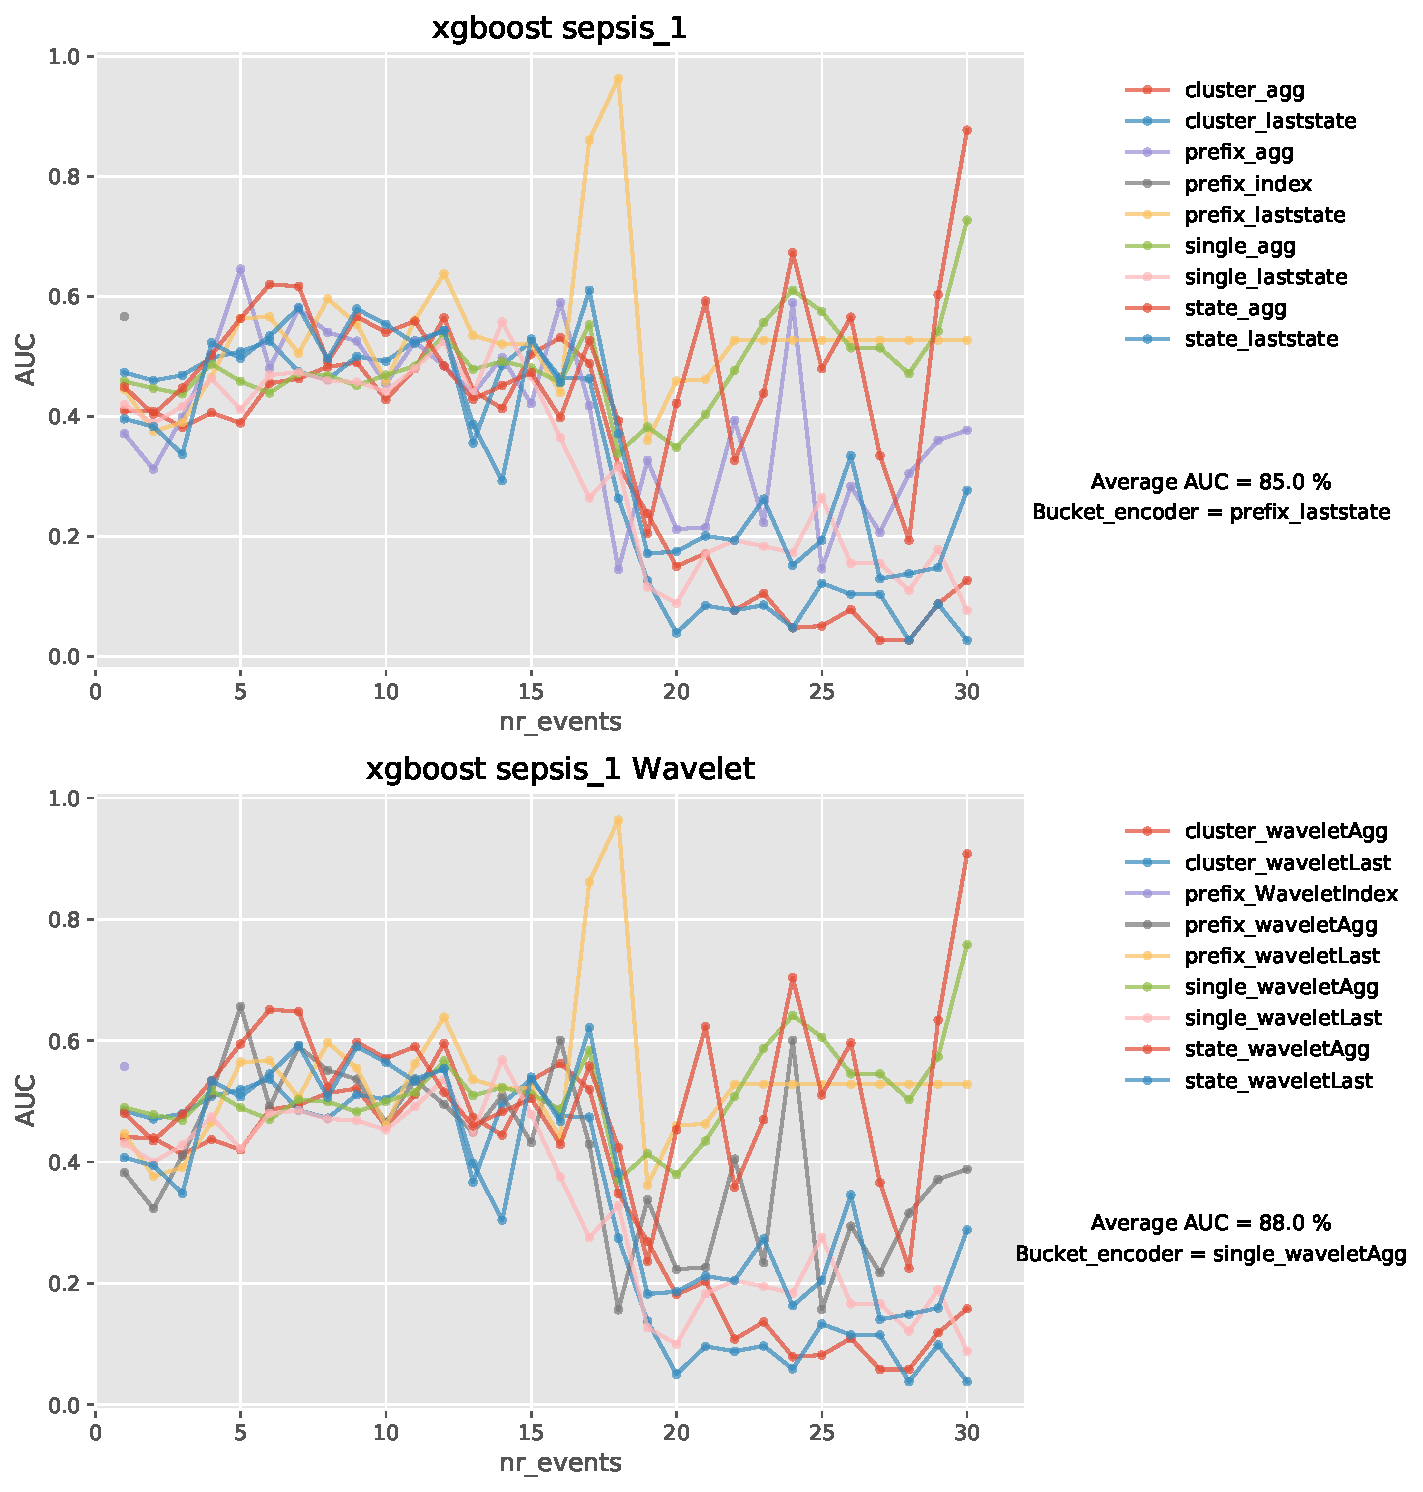
\includegraphics[width=\linewidth]{images/wavelet/graphs2/sepsis_1.pdf}=
		\caption{Wavelet sepsis\_1} \label{fig:sepsisw}
	\end{subfigure}\hspace*{\fill}
	\begin{subfigure}{0.48\textwidth}
		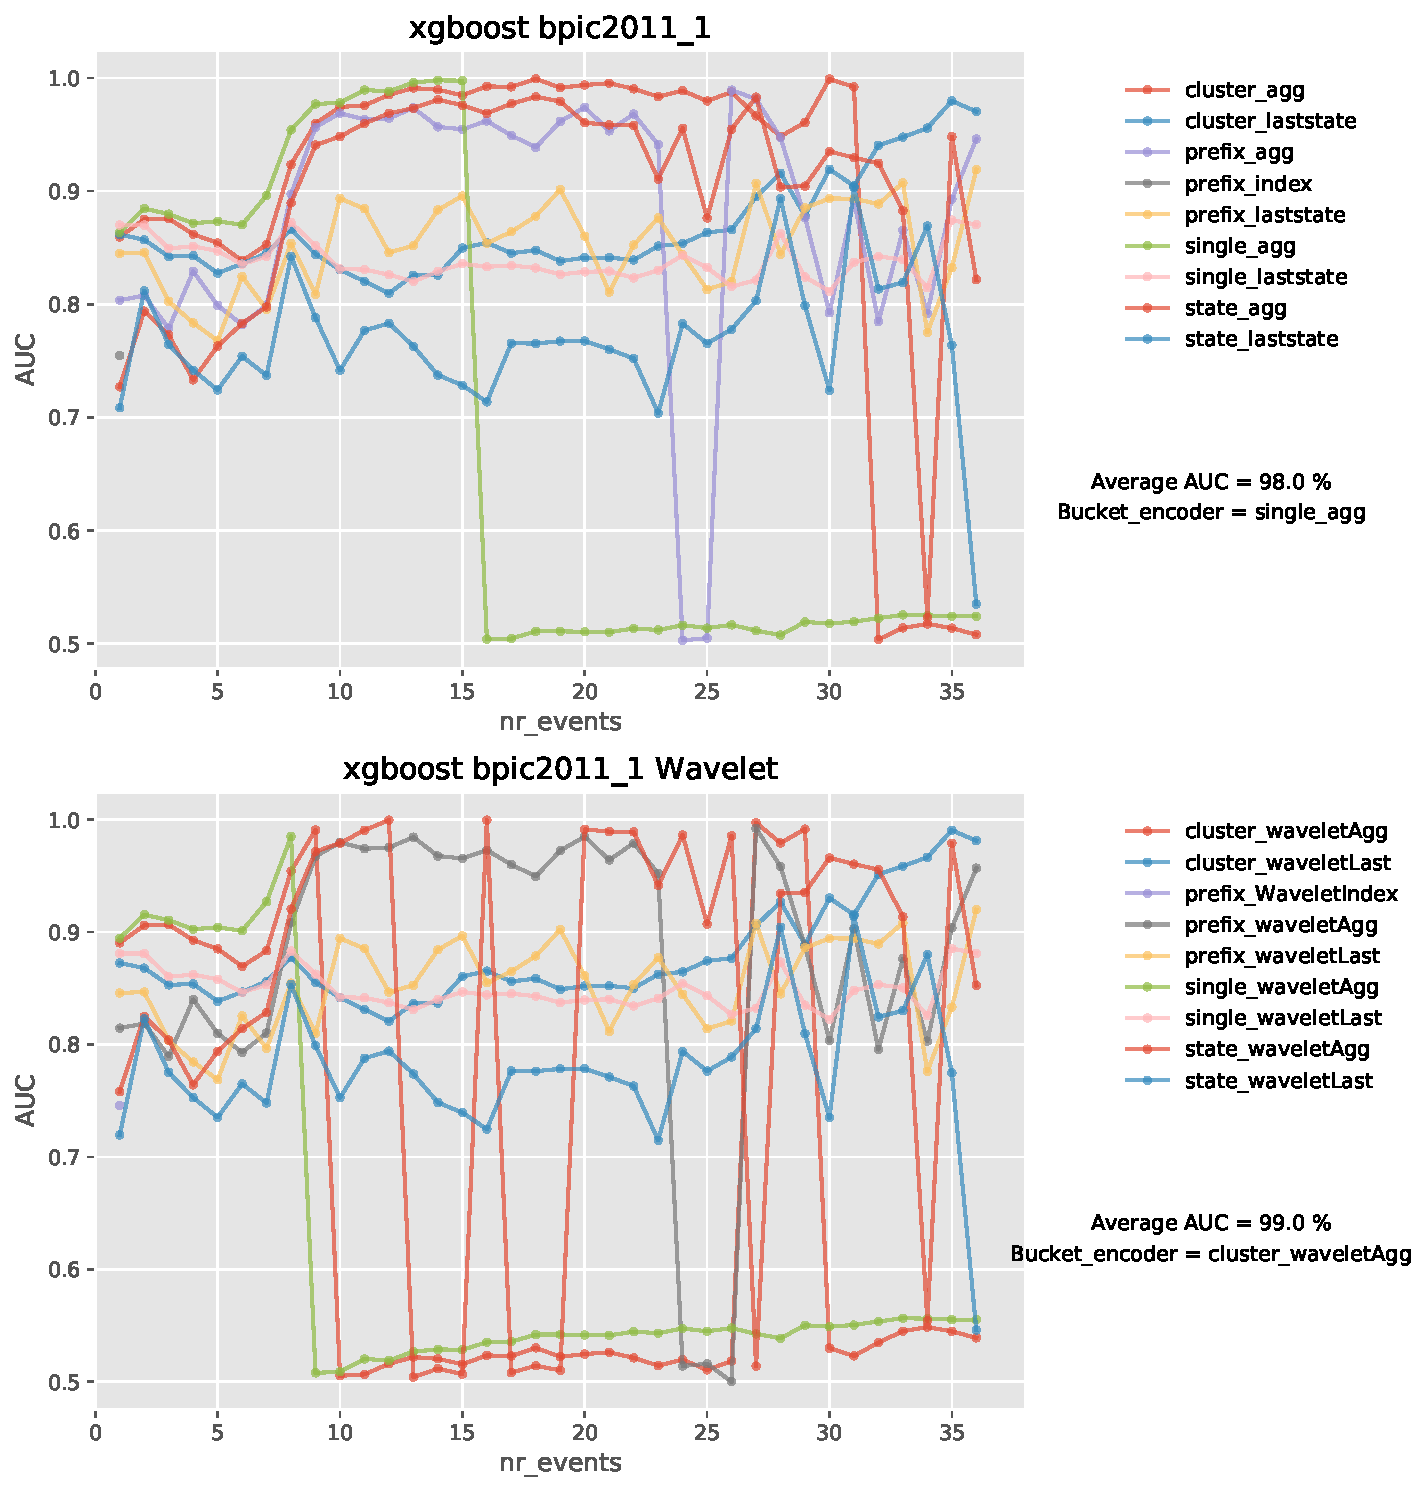
\includegraphics[width=\linewidth]{images/wavelet/graphs2/bpic2011_1.pdf}
		\caption{Wavelet bpic2011} \label{fig:b11w}
	\end{subfigure}
	
	\medskip
	\begin{subfigure}{0.48\textwidth}
		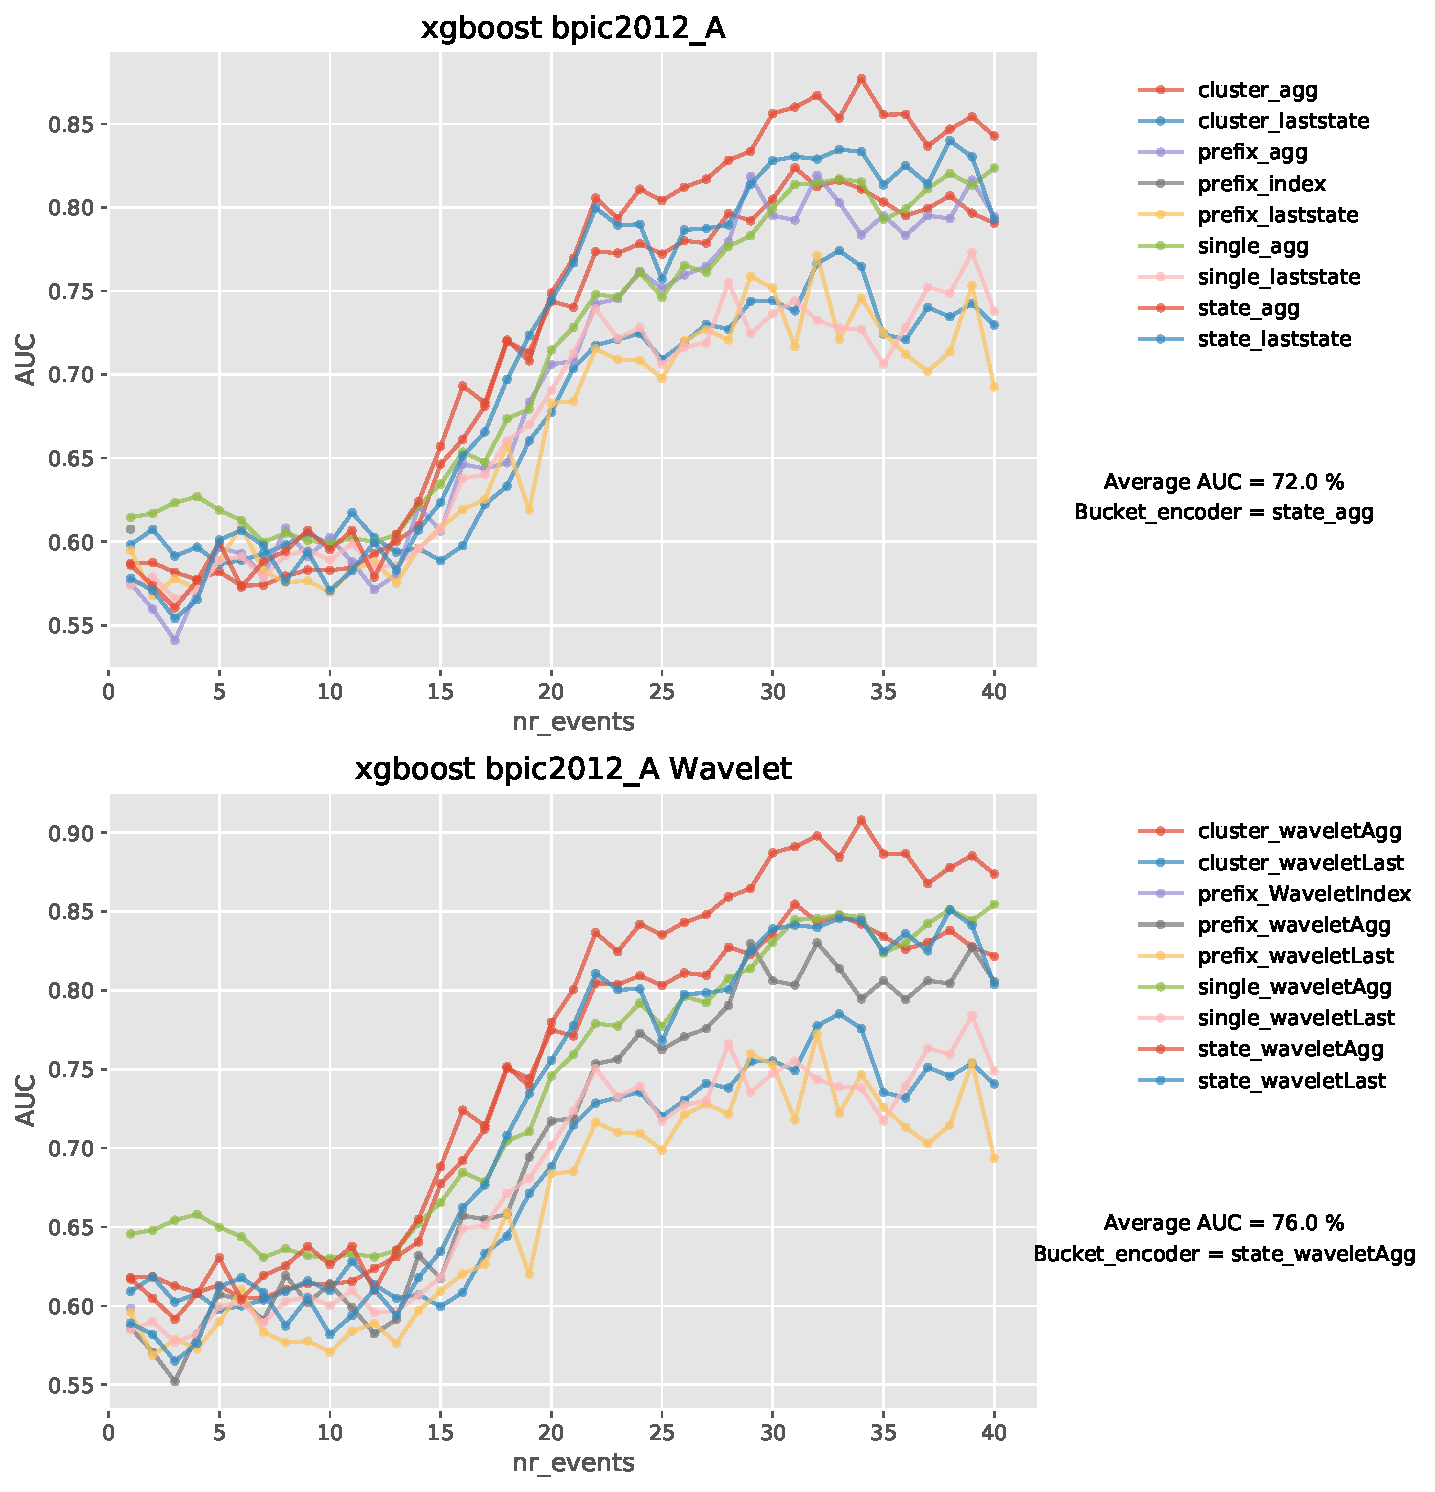
\includegraphics[width=\linewidth]{images/wavelet/graphs2/bpic2012_A.pdf}
		\caption{Wavelet bpic2012\_A} \label{fig:b12aw}
	\end{subfigure}\hspace*{\fill}
	\begin{subfigure}{0.48\textwidth}
		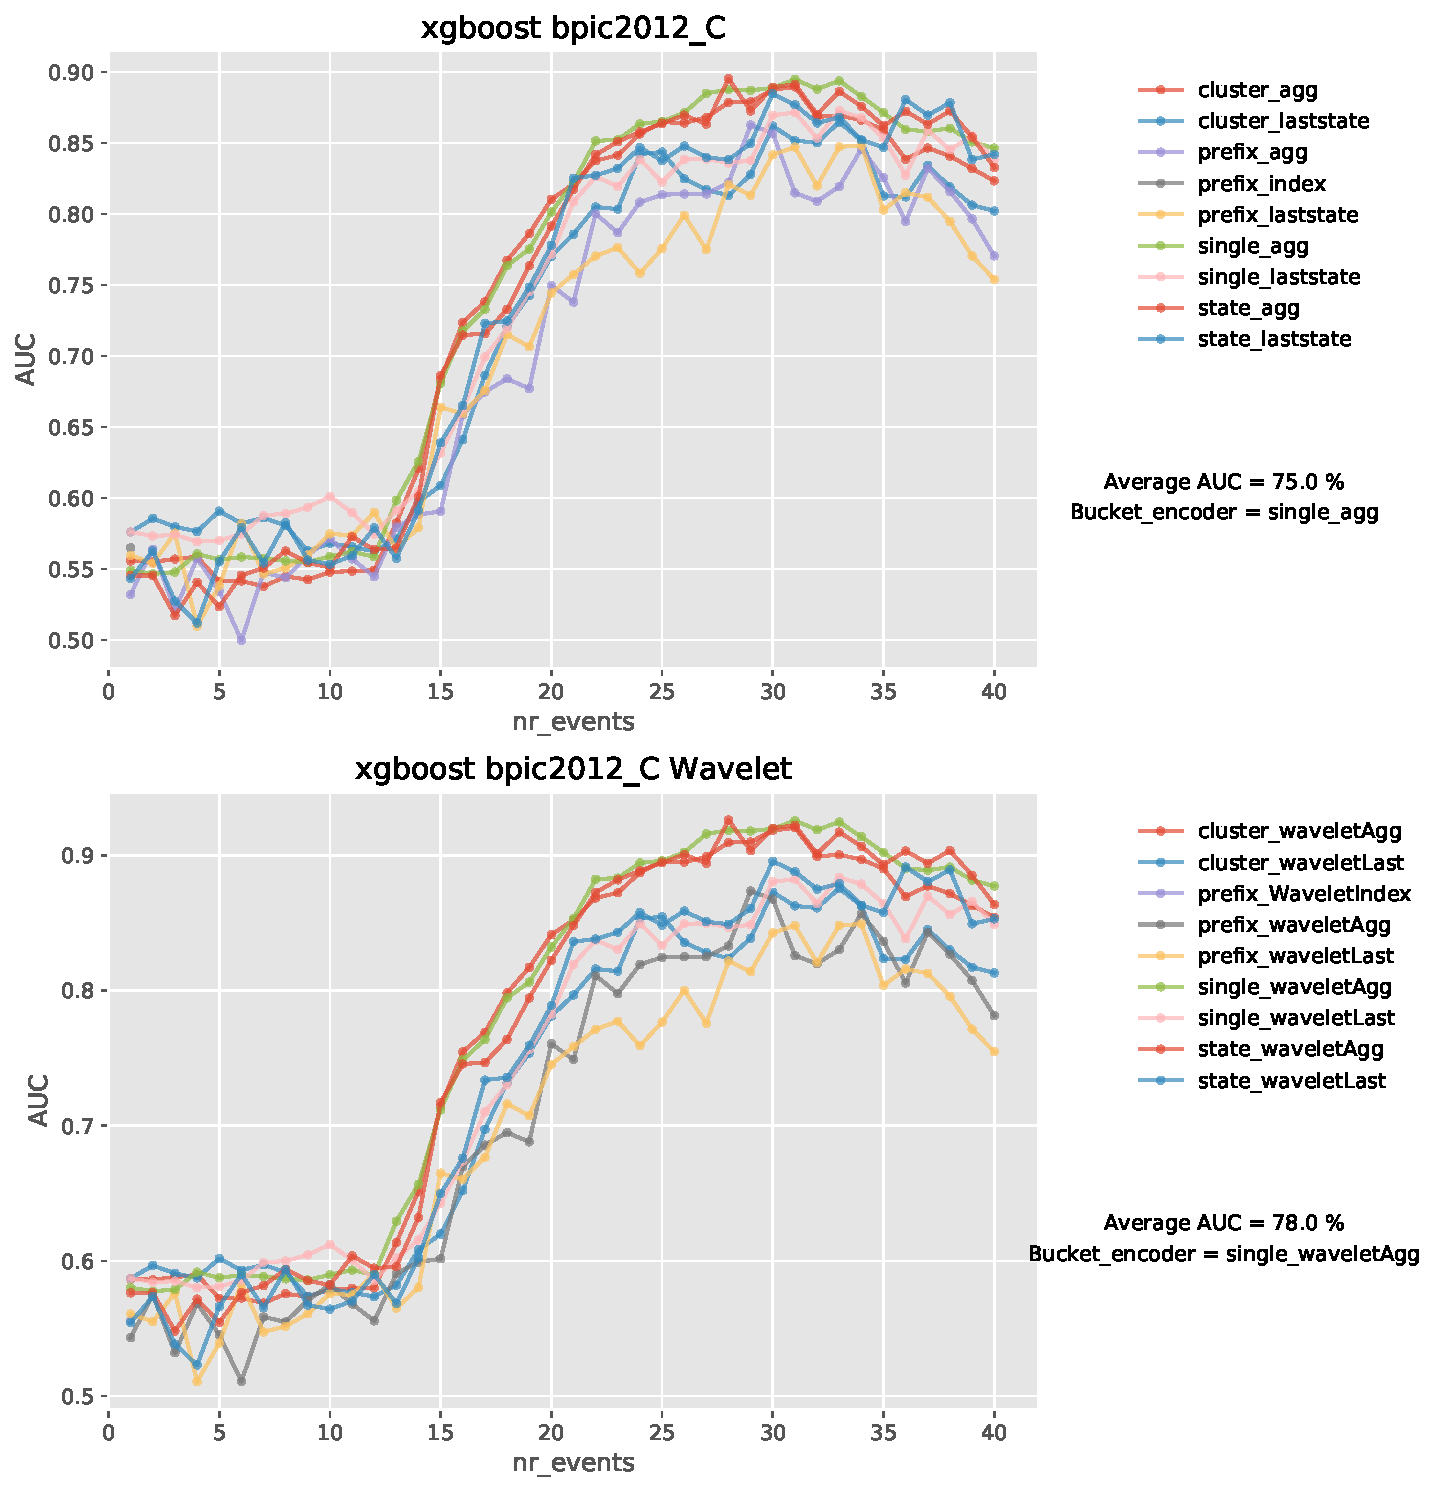
\includegraphics[width=\linewidth]{images/wavelet/graphs2/bpic2012_C.pdf}
		\caption{Wavelet bpic2012\_C} \label{fig:b12cw}
	\end{subfigure}	
\caption{Comparing XGBoost before and after adding wavelet encoding on all event logs.}
\label{fig:r1w}
\end{figure}



\begin{figure}[!htbp] % "[t!]" placement specifier just for this example
	
	\begin{subfigure}{0.48\textwidth}
		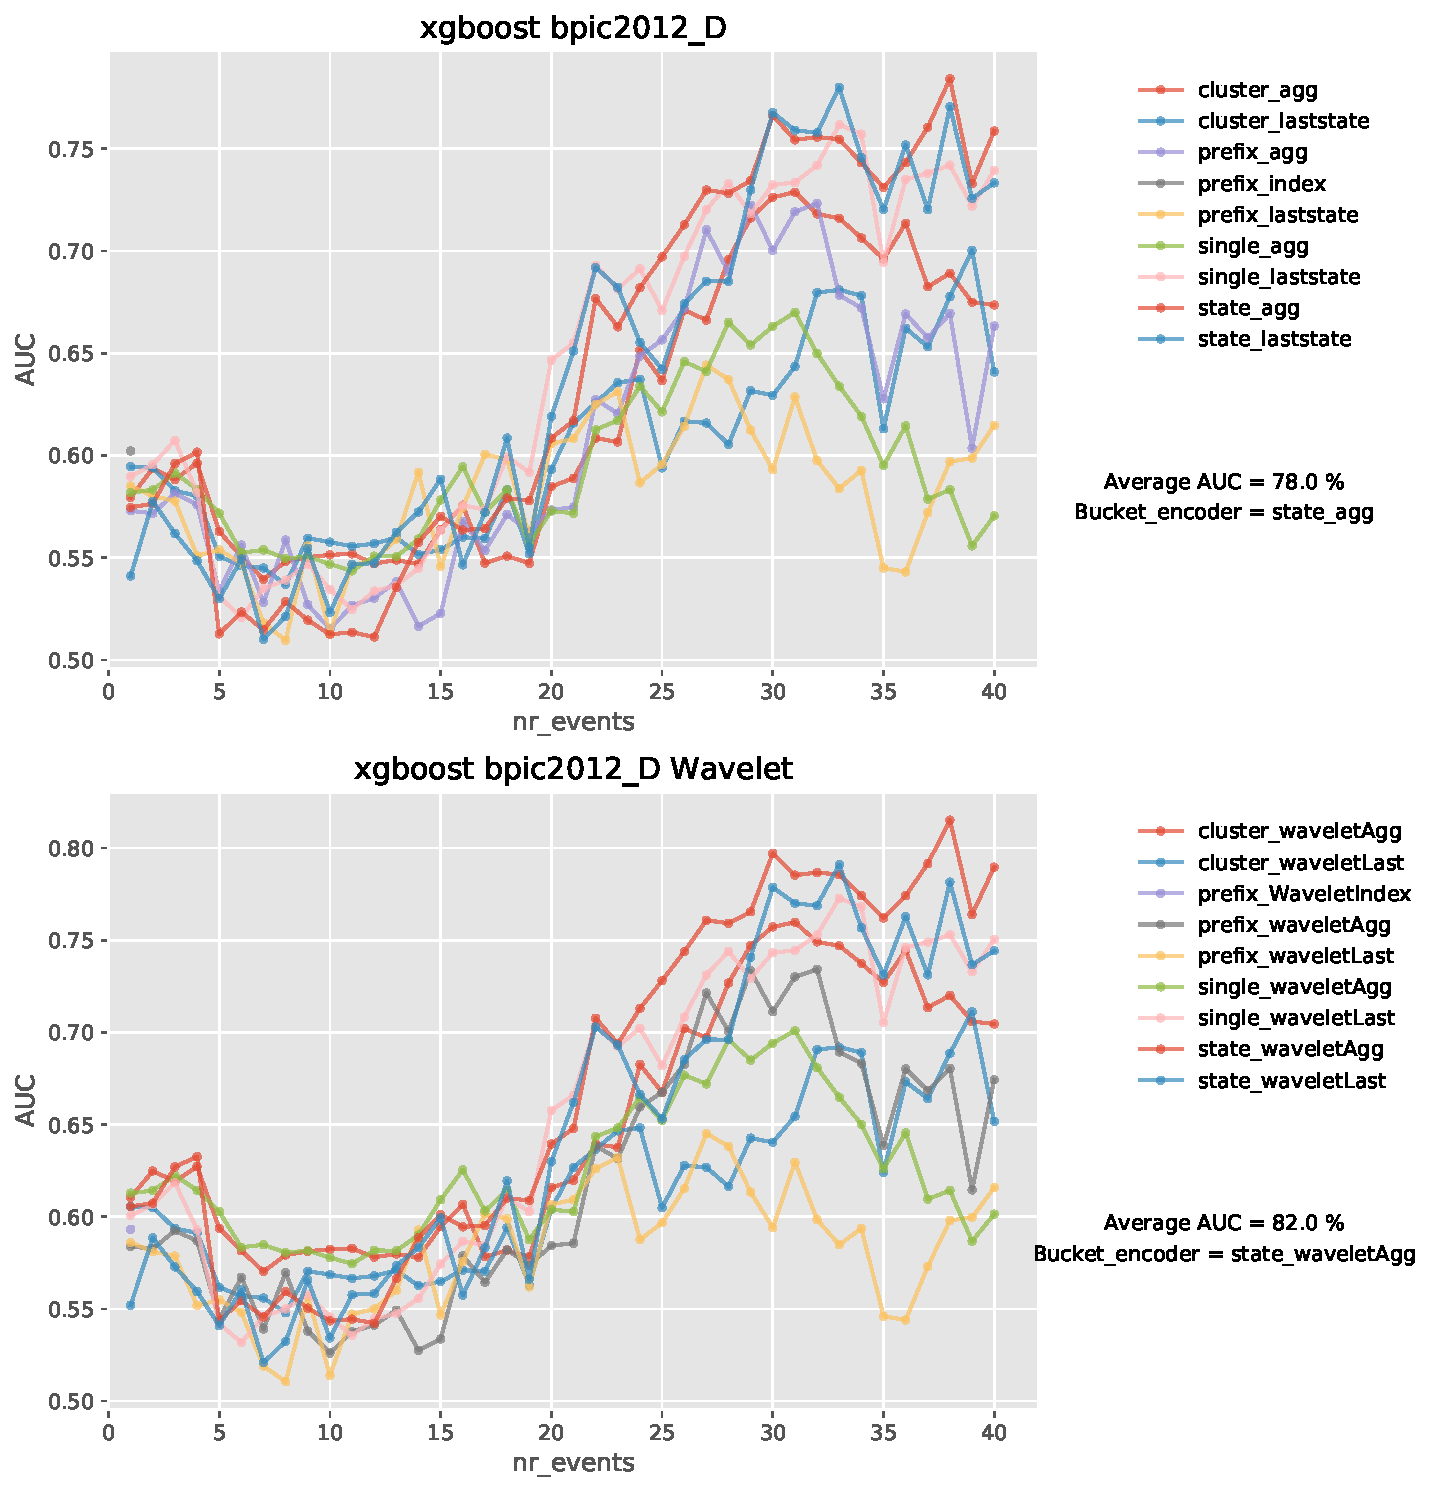
\includegraphics[width=\linewidth]{images/wavelet/graphs2/bpic2012_D.pdf}
		\caption{Wavelet bpic2012\_D} \label{fig:b12dw}
	\end{subfigure}\hspace*{\fill}
	\begin{subfigure}{0.48\textwidth}
		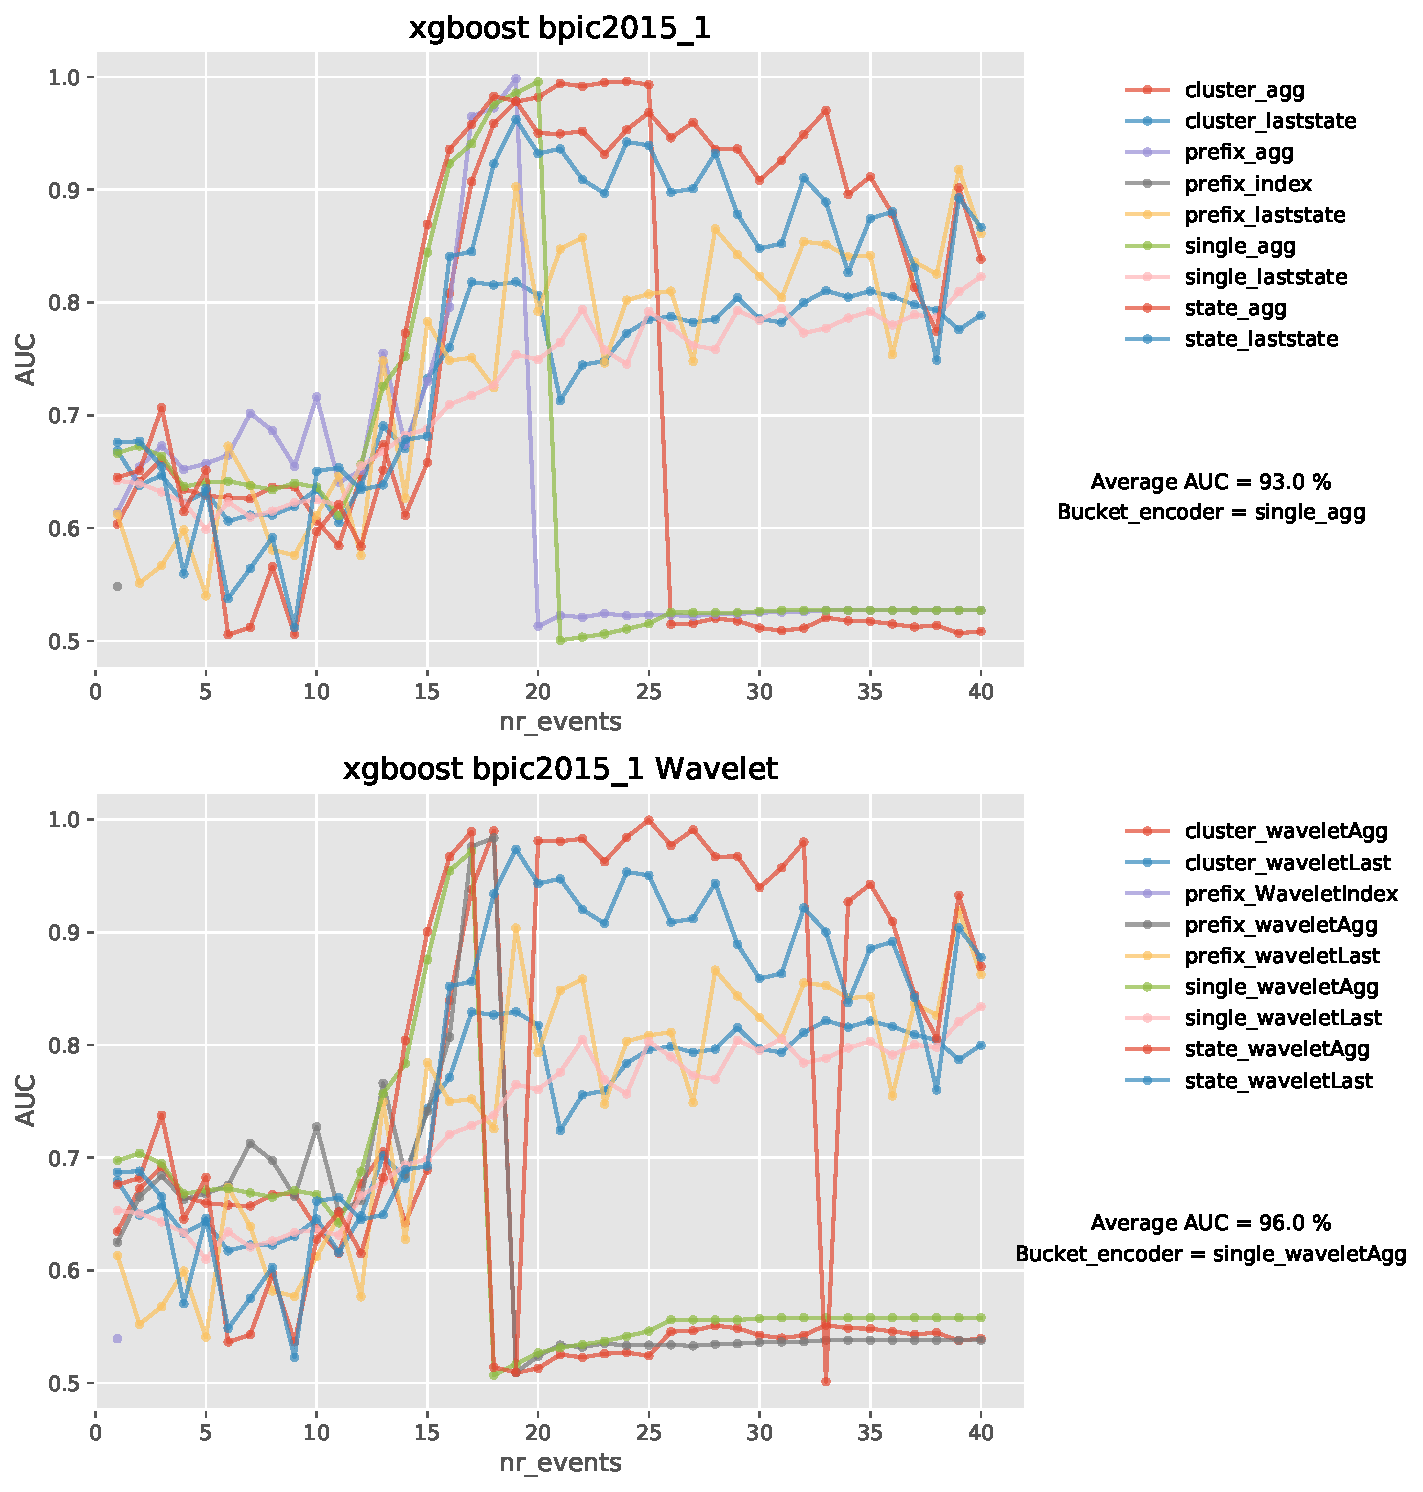
\includegraphics[width=\linewidth]{images/wavelet/graphs2/bpic2015_1.pdf}
		\caption{Wavelet bpic2015} \label{fig:b151w}
	\end{subfigure}
	
	\begin{subfigure}{0.48\textwidth}
		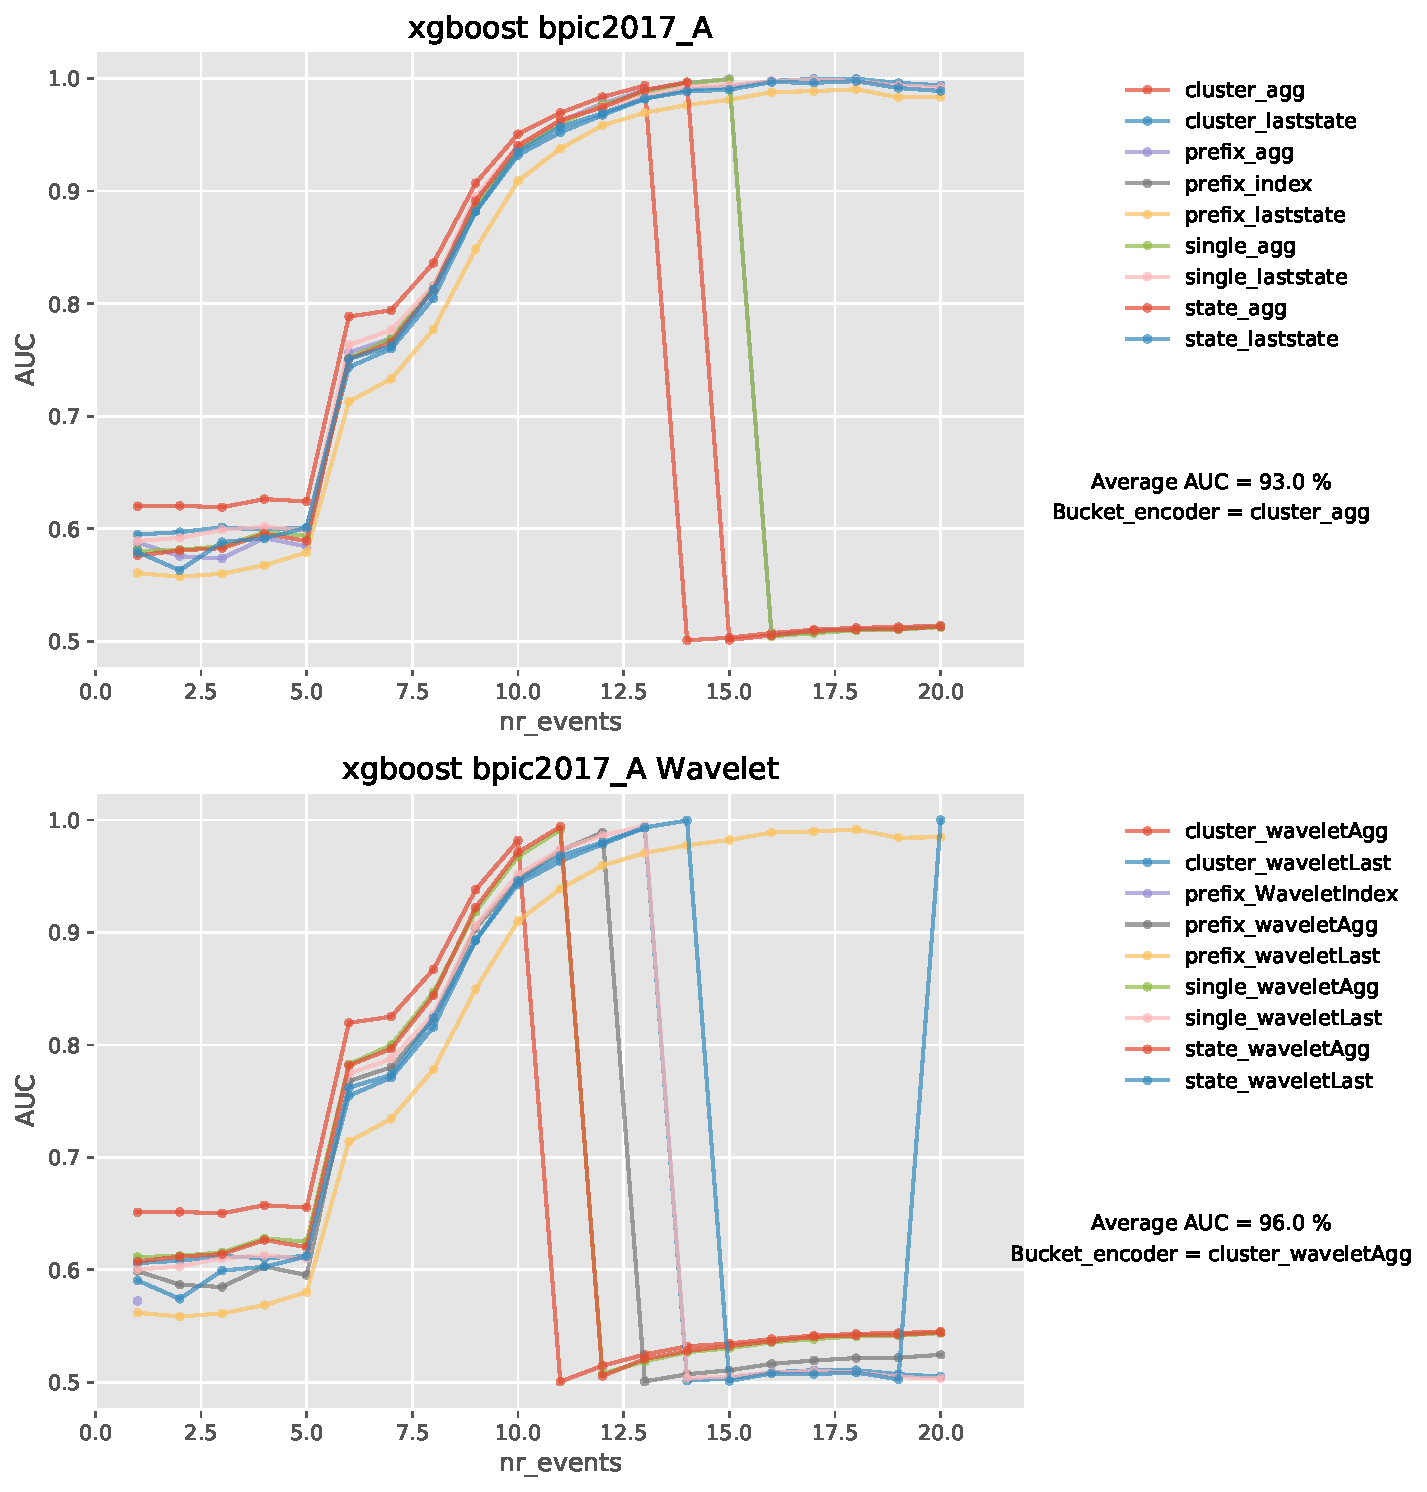
\includegraphics[width=\linewidth]{images/wavelet/graphs2/bpic2017_A.pdf}
		\caption{Wavelet bpic2017\_A} \label{fig:b17aw}
	\end{subfigure}\hspace*{\fill}
	\begin{subfigure}{0.48\textwidth}
		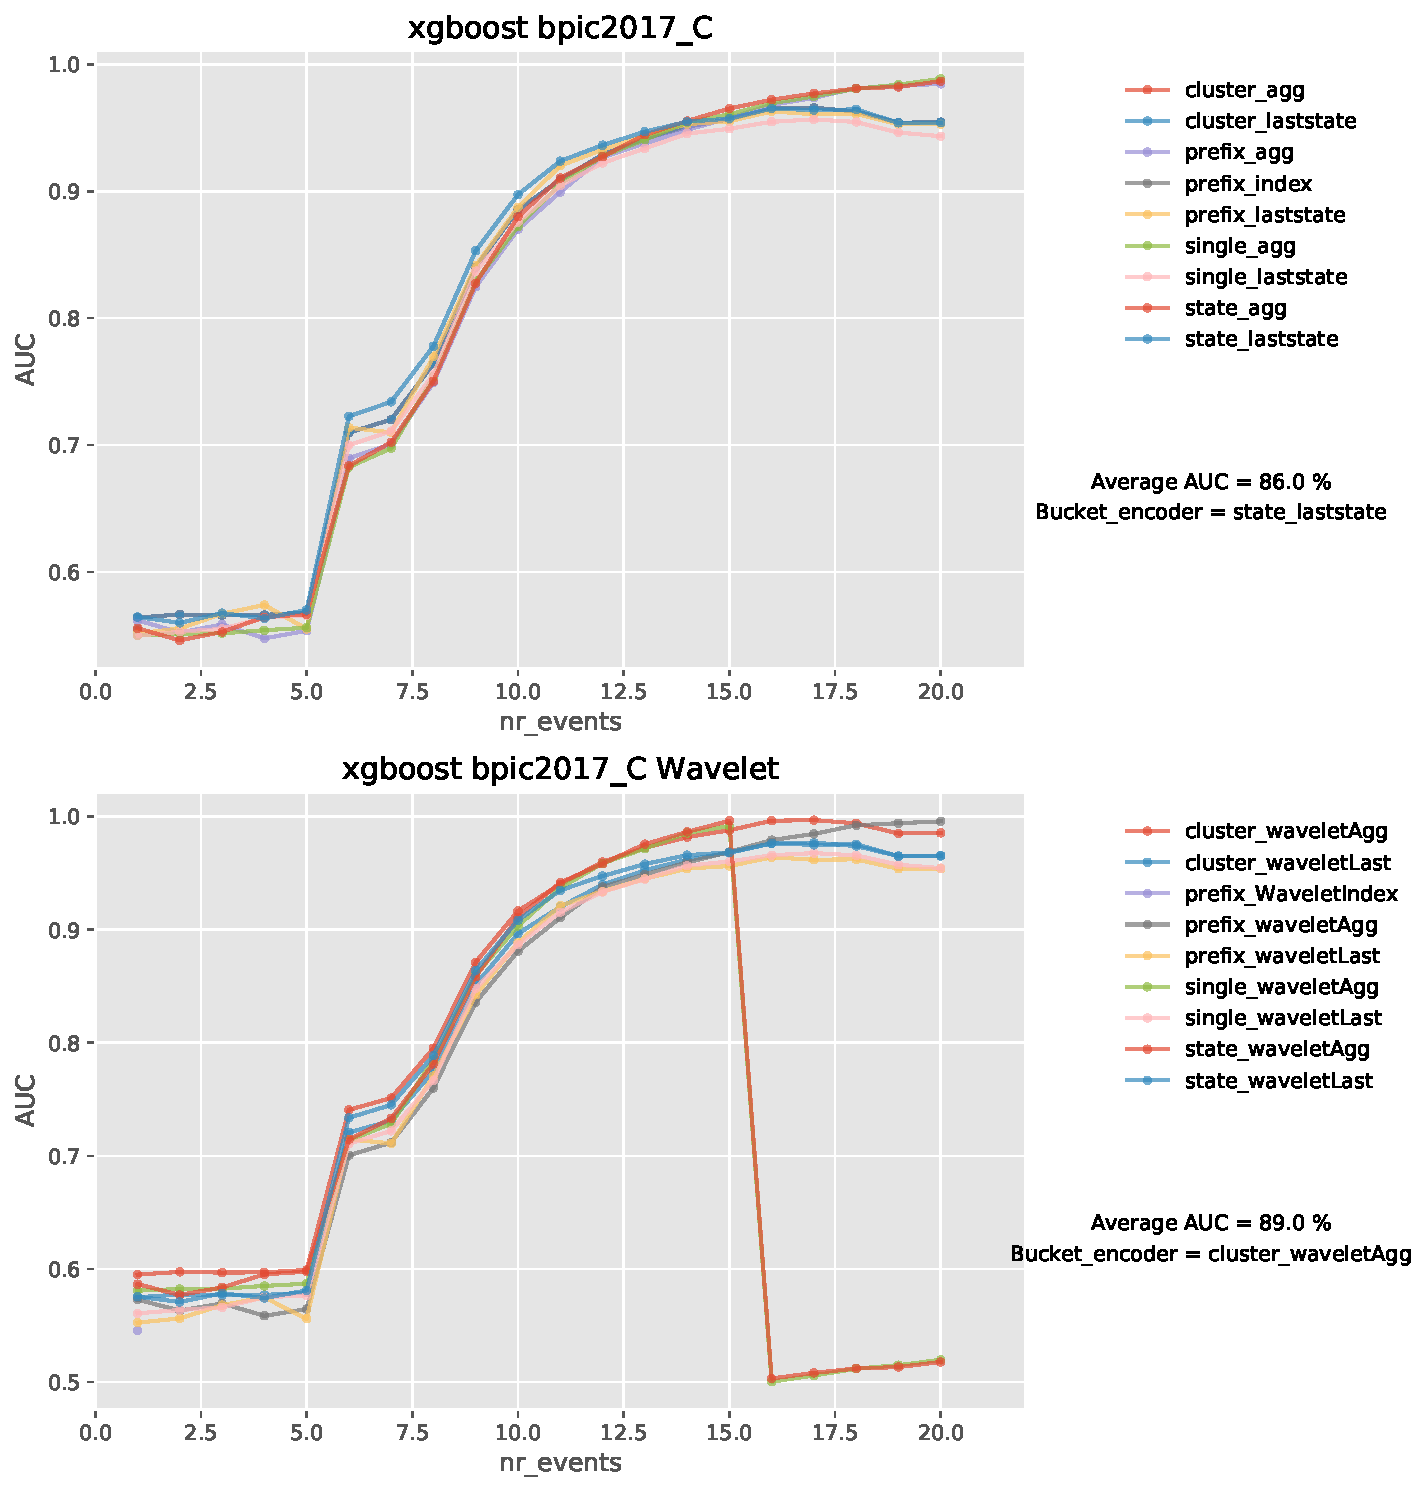
\includegraphics[width=\linewidth]{images/wavelet/graphs2/bpic2017_C.pdf}
		\caption{Wavelet bpic2017\_C} \label{fig:b17cw}
	\end{subfigure}
	\caption{Comparing XGBoost before and after adding wavelet encoding on all event logs (\textit{continued}).}
	\label{fig:r2w}
\end{figure}


\begin{figure}[!htbp] % "[t!]" placement specifier just for this example

	\begin{subfigure}{0.48\textwidth}
		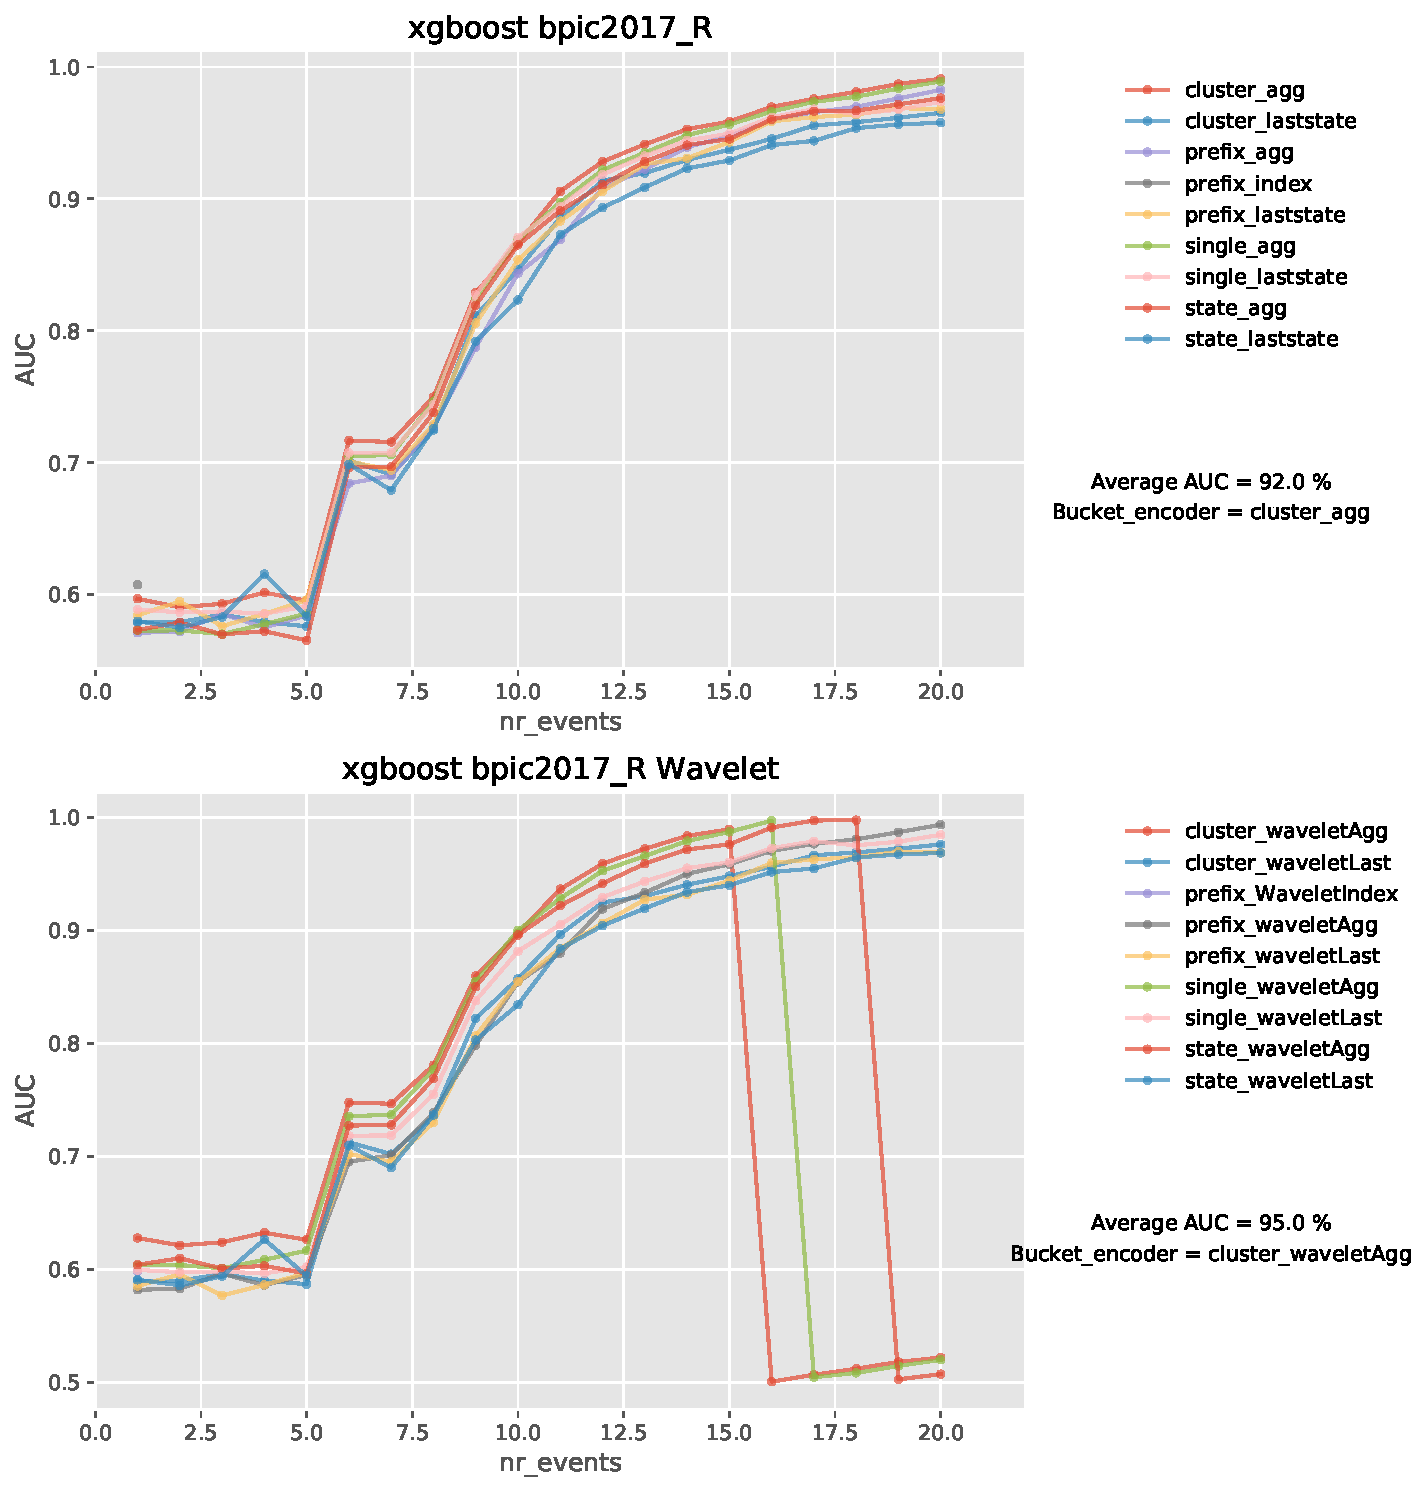
\includegraphics[width=\linewidth]{images/wavelet/graphs2/bpic2017_R.pdf}
		\caption{Wavelet bpic2017\_R} \label{fig:b17rw}
	\end{subfigure}\hspace*{\fill}
	\begin{subfigure}{0.48\textwidth}
		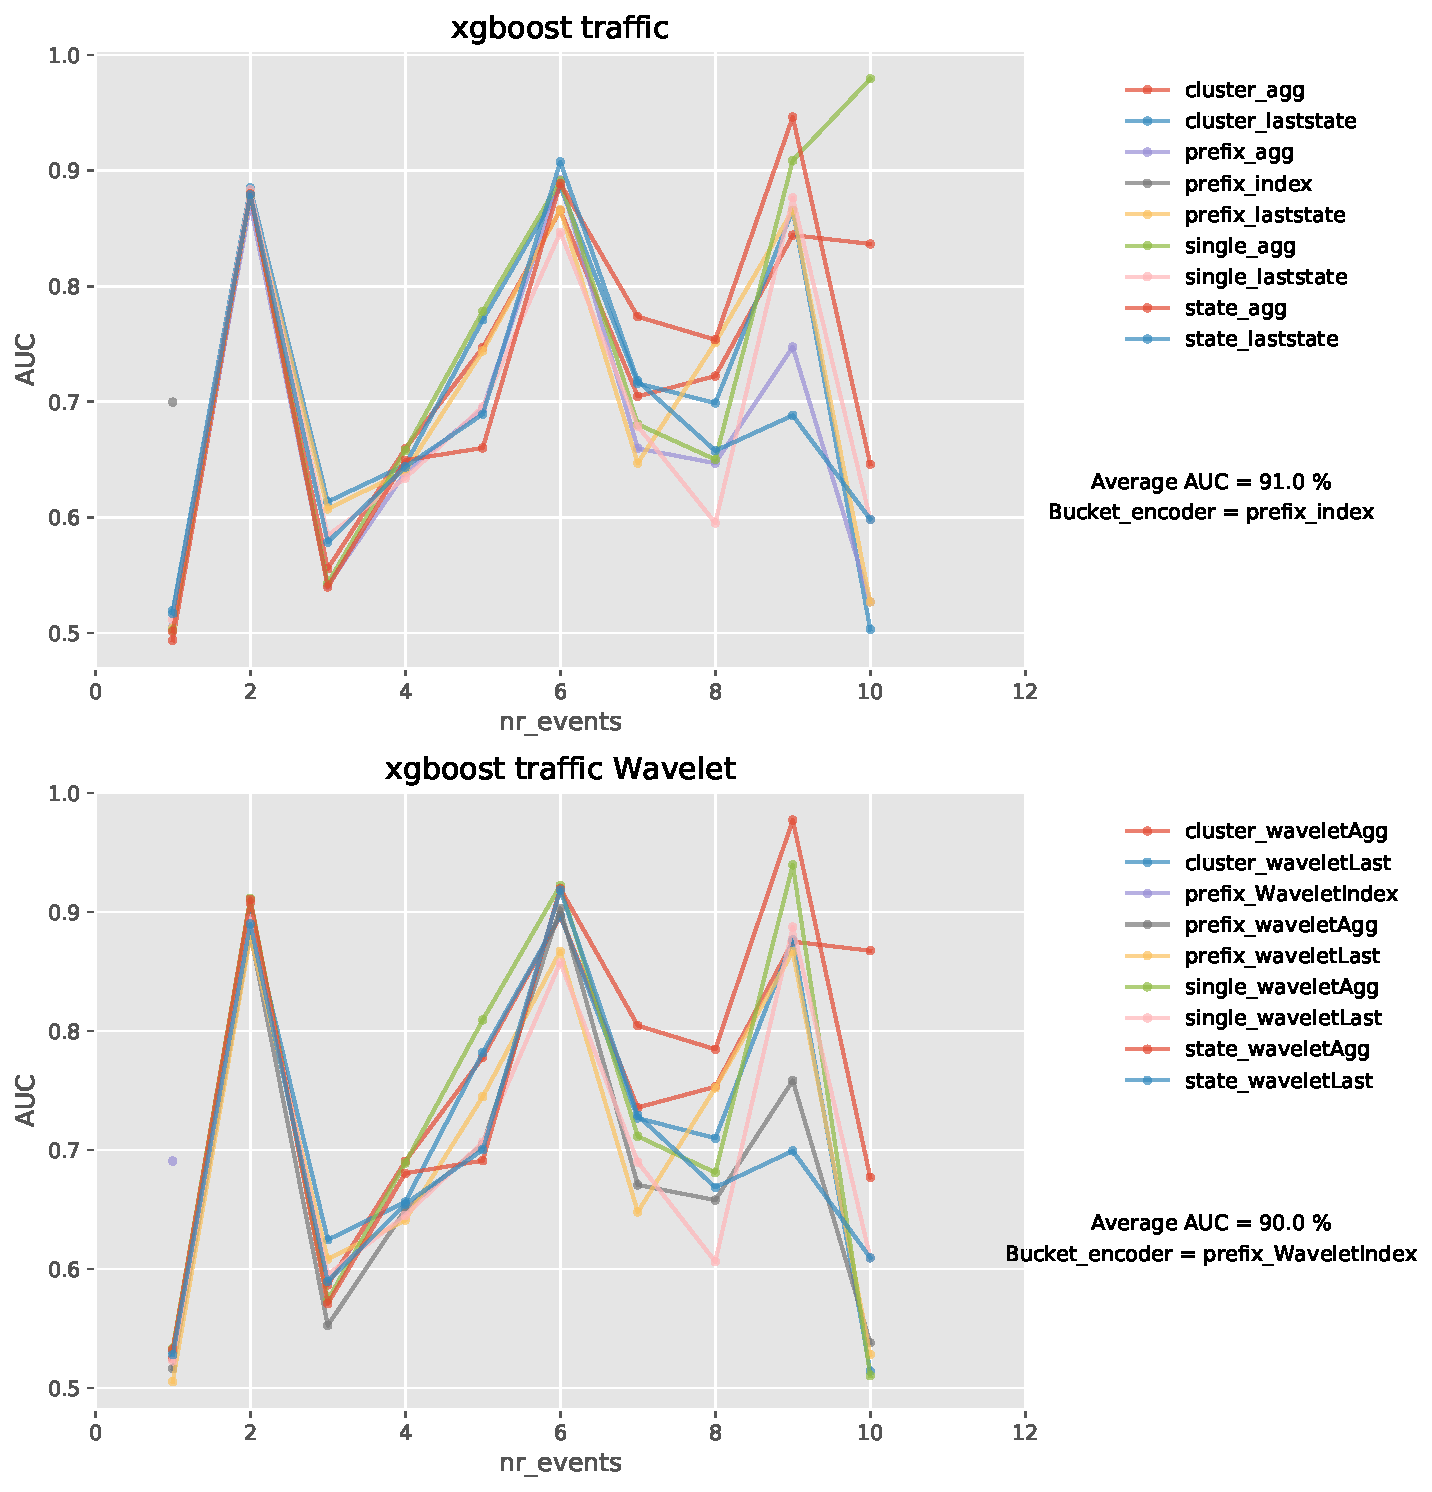
\includegraphics[width=\linewidth]{images/wavelet/graphs2/traffic.pdf}
		\caption{Wavelet traffic} \label{fig:trafw}
	\end{subfigure}
	
	\begin{subfigure}{0.48\textwidth}
		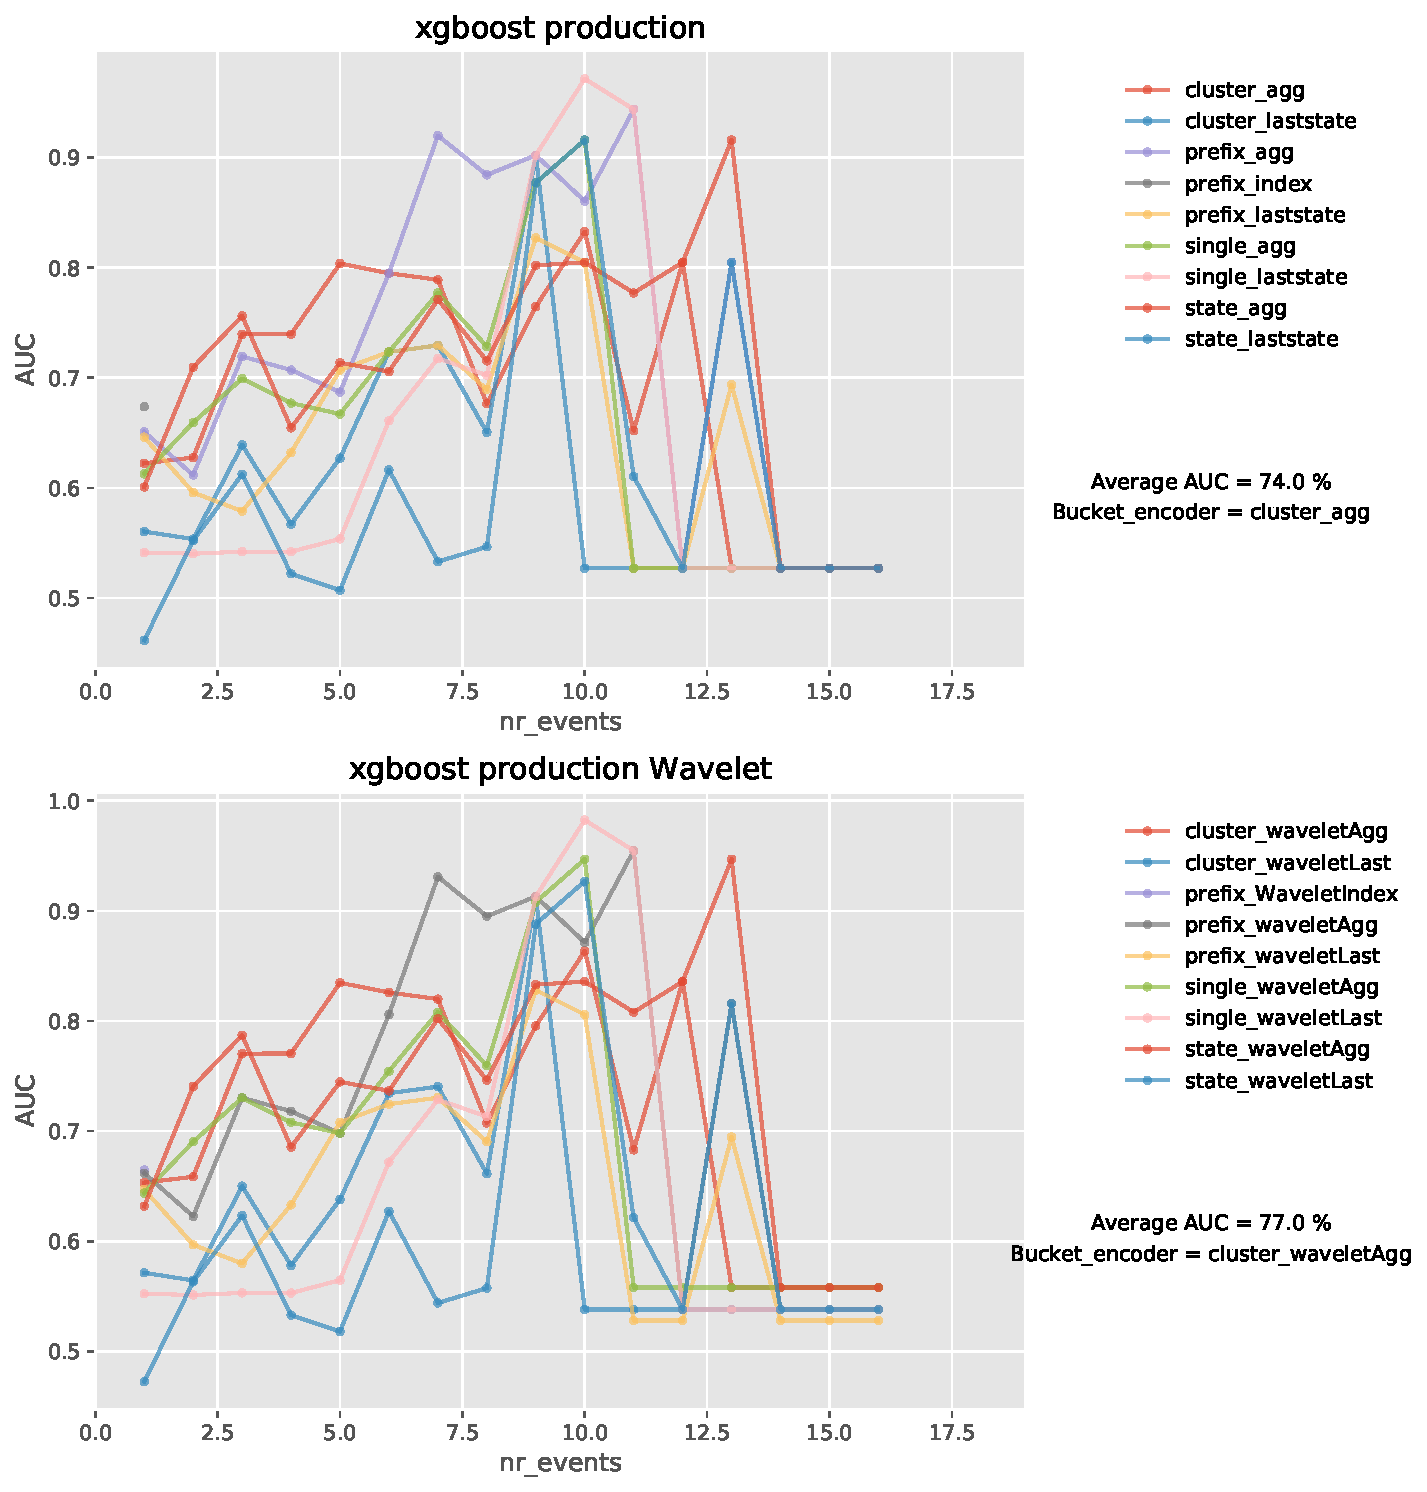
\includegraphics[width=\linewidth]{images/wavelet/graphs2/production.pdf}
		\caption{Wavelet Production} \label{fig:prow}
	\end{subfigure}\hspace*{\fill}
	\caption{Comparing XGBoost before and after adding wavelet encoding on all event logs (\textit{continued})}
\label{fig:r3w}
\end{figure}


\clearpage

\subsection{Contribution 3: Inter-case features results}
In this section, we added our proposed inter-case features that include three different categories, i.e. workload, demand intensity, and temporal context features, as shown in figure \ref{fig:interr}.

\begin{figure}[!htb]
	\begin{center}
		\resizebox{10cm}{!}{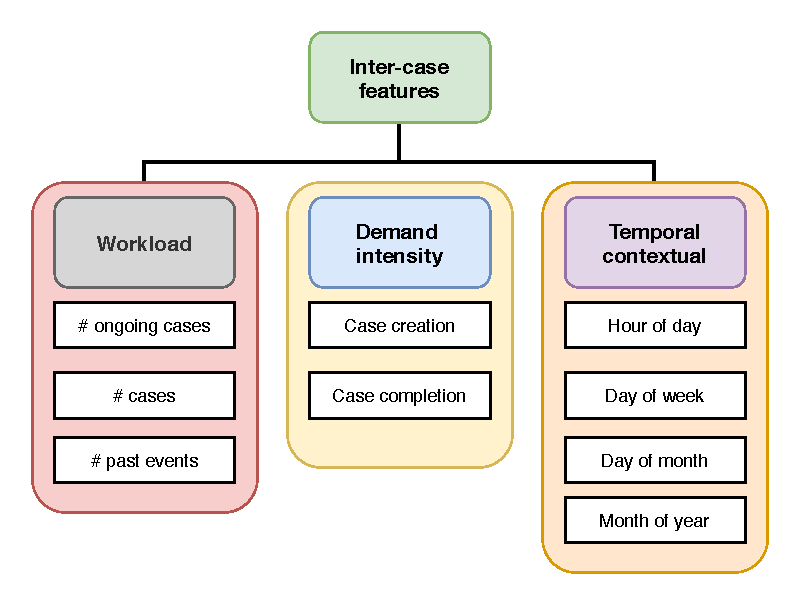
\includegraphics{images/general/inter1.pdf}}
		\caption[Inter-case features]{Categorization of inter-case features that we propose in this thesis, i.e. workload, demand intensity, and temporal context features.
		}
		\label{fig:interr}
	\end{center}
\end{figure}




To report the overall AUC after adding inter-case features, we used the same experiments that we did in figure \ref{fig:cate}. We calculated all prediction scores across all prefix lengths, and after that, we calculated the average score for all predictions based on the number of tested prefixes for each case as we did in our previously proposed methods. 

Table \ref{tab:interc} show collected results of CatBoost classifier with inter-case features in terms of AUC and F-score, and for XGBoost, RF, Logit, and SVM results are shown in Tables \ref{tab:interx}, \ref{tab:interr}, \ref{tab:interl}, and \ref{tab:inters}.


\begin{table}[!htbp]
	\caption{Overall AUC (F-score) for \textbf{CatBoost plus Inter-case features}}
	\label{tab:interc}
	
	
	\centering
	\resizebox{0.8\textwidth}{!}{%
		\begin{tabular}{llllllll}
			
			\toprule
			& \multicolumn{5}{c}{catboost}
			\\
			& bpic2015\_2 & bpic2015\_4 & bpic2011\_4 & bpic2017\_r & bpic2012\_d & bpic2012\_a
			\\ \midrule
			cluster\_laststate & $0.85$ ${(0.23)}$ & $0.67$ ${(0.35)}$ & $0.96$ ${(0.87)}$ & $0.93$ ${(0.69)}$ & $0.67$ ${(0.3)}$ & $0.81$ ${(0.81)}$ \\
			cluster\_agg & $0.99$ ${(0.67)}$ & $0.7$ ${(0.33)}$ & $0.96$ ${(0.87)}$ & $0.93$ ${(0.69)}$ & $0.7$ ${(0.29)}$ & $0.82$ ${(0.8)}$ \\
			single\_agg & $0.89$ ${(0.61)}$ & $0.69$ ${(0.33)}$ & $0.98$ ${(0.94)}$ & $0.91$ ${(0.65)}$ & $0.65$ ${(0.25)}$ & $0.8$ ${(0.81)}$ \\
			prefix\_agg & $0.94$ ${(0.47)}$ & $0.67$ ${(0.33)}$ & $\mathbf{0.99}$ $\mathbf{(0.89)}$  & $0.93$ ${(0.67)}$ & $0.62$ ${(0.2)}$ & $0.83$ ${(0.83)}$ \\
			prefix\_laststate & $0.85$ ${(0.31)}$ & $0.7$ ${(0.26)}$ & $0.98$ ${(0.89)}$ & $0.92$ ${(0.68)}$ & $-$  & $0.83$ ${(0.83)}$ \\
			single\_laststate & $0.88$ ${(0.39)}$ & $0.69$ ${(0.26)}$ & $\mathbf{0.99}$ $\mathbf{(0.93)}$  & $0.92$ ${(0.67)}$ & $-$  & $0.82$ ${(0.83)}$ \\
			prefix\_index & $0.73$ ${(0.54)}$ & $0.72$ ${(0.32)}$ & $\mathbf{0.99}$ $\mathbf{(0.88)}$  & $0.84$ ${(0.42)}$ & $-$  & $0.83$ ${(0.7)}$ \\
			state\_agg & $0.85$ ${(0.32)}$ & $\mathbf{0.76}$ $\mathbf{(0.37)}$  & $0.92$ ${(0.84)}$ & $0.92$ ${(0.67)}$ & $0.67$ ${(0.29)}$ & $0.83$ ${(0.82)}$ \\
			state\_laststate & $0.83$ ${(0.33)}$ & $0.74$ ${(0.33)}$ & $0.91$ ${(0.81)}$ & $0.91$ ${(0.65)}$ & $-$  & $0.83$ ${(0.81)}$ \\
			\bottomrule
			\toprule
			& \multicolumn{5}{c}{catboost}
			\\
			& bpic2015\_3 & bpic2011\_3 & bpic2011\_2 & sepsis\_2 & bpic2015\_1 & bpic2015\_5
			\\ \midrule
			cluster\_laststate & $0.63$ ${(0.27)}$ & $0.98$ ${(0.93)}$ & $0.88$ ${(0.83)}$ & $0.5$ ${(0.0)}$ & $0.72$ ${(0.38)}$ & $0.69$ ${(0.45)}$ \\
			cluster\_agg & $0.6$ ${(0.2)}$ & $0.99$ ${(0.95)}$ & $0.98$ ${(0.85)}$ & $0.5$ ${(0.0)}$ & $0.84$ ${(0.56)}$ & $0.69$ ${(0.51)}$ \\
			single\_agg & $0.6$ ${(0.22)}$ & $0.98$ ${(0.93)}$ & $0.86$ ${(0.79)}$ & $0.5$ ${(0.0)}$ & $0.68$ ${(0.34)}$ & $0.67$ ${(0.49)}$ \\
			prefix\_agg & $0.61$ ${(0.21)}$ & $0.98$ ${(0.96)}$ & $0.84$ ${(0.8)}$ & $0.5$ ${(0.0)}$ & $0.72$ ${(0.38)}$ & $0.71$ ${(0.47)}$ \\
			prefix\_laststate & $0.6$ ${(0.19)}$ & $0.99$ ${(0.97)}$ & $0.83$ ${(0.83)}$ & $0.5$ ${(0.0)}$ & $0.71$ ${(0.36)}$ & $0.69$ ${(0.49)}$ \\
			single\_laststate & $0.6$ ${(0.27)}$ & $0.98$ ${(0.95)}$ & $0.88$ ${(0.81)}$ & $0.5$ ${(0.0)}$ & $0.86$ ${(0.5)}$ & $0.71$ ${(0.53)}$ \\
			prefix\_index & $0.6$ ${(0.23)}$ & $0.99$ ${(0.97)}$ & $0.87$ ${(0.86)}$ & $\mathbf{0.98}$ $\mathbf{(0.96)}$  & $0.56$ ${(0.15)}$ & $\mathbf{0.72}$ $\mathbf{(0.36)}$  \\
			state\_agg & $0.61$ ${(0.19)}$ & $0.99$ ${(0.94)}$ & $0.53$ ${(0.74)}$ & $0.33$ ${(0.0)}$ & $0.75$ ${(0.44)}$ & $0.69$ ${(0.5)}$ \\
			state\_laststate & $0.59$ ${(0.32)}$ & $0.99$ ${(0.9)}$ & $0.57$ ${(0.75)}$ & $0.33$ ${(0.0)}$ & $0.73$ ${(0.46)}$ & $0.7$ ${(0.55)}$ \\
			\bottomrule
			\toprule
			& \multicolumn{5}{c}{catboost}
			\\
			& sepsis\_1 & bpic2017\_c & sepsis\_3 & bpic2012\_c & production & bpic2011\_1
			\\ \midrule
			cluster\_laststate & $0.46$ ${(0.03)}$ & $\mathbf{0.99}$ $\mathbf{(0.96)}$  & $\mathbf{0.98}$ $\mathbf{(0.9)}$  & $0.97$ ${(0.88)}$ & $0.69$ ${(0.6)}$ & $0.99$ ${(0.84)}$ \\
			cluster\_agg & $0.47$ ${(0.05)}$ & $\mathbf{0.99}$ $\mathbf{(0.97)}$  & $\mathbf{0.98}$ $\mathbf{(1.0)}$  & $0.97$ ${(0.87)}$ & $0.67$ ${(0.62)}$ & $0.99$ ${(0.87)}$ \\
			single\_agg & $0.52$ ${(0.1)}$ & $\mathbf{0.99}$ $\mathbf{(0.97)}$  & $\mathbf{0.98}$ $\mathbf{(0.91)}$  & $0.97$ ${(0.87)}$ & $0.67$ ${(0.58)}$ & $0.97$ ${(0.86)}$ \\
			prefix\_agg & $0.45$ ${(0.01)}$ & $\mathbf{0.99}$ $\mathbf{(0.97)}$  & $\mathbf{0.98}$ $\mathbf{(0.94)}$  & $0.97$ ${(0.87)}$ & $0.66$ ${(0.6)}$ & $0.99$ ${(0.93)}$ \\
			prefix\_laststate & $0.48$ ${(0.02)}$ & $\mathbf{0.99}$ $\mathbf{(0.97)}$  & $\mathbf{0.98}$ $\mathbf{(0.96)}$  & $0.97$ ${(0.87)}$ & $\mathbf{0.78}$ $\mathbf{(0.55)}$  & $0.99$ ${(0.9)}$ \\
			single\_laststate & $0.55$ ${(0.17)}$ & $\mathbf{0.99}$ $\mathbf{(0.97)}$  & $\mathbf{0.98}$ $\mathbf{(0.94)}$  & $0.97$ ${(0.88)}$ & $0.77$ ${(0.59)}$ & $0.97$ ${(0.74)}$ \\
			prefix\_index & $0.51$ ${(0.0)}$ & $\mathbf{0.99}$ $\mathbf{(0.96)}$  & $\mathbf{0.98}$ $\mathbf{(1.0)}$  & $0.97$ ${(0.9)}$ & $0.75$ ${(0.64)}$ & $\mathbf{0.98}$ $\mathbf{(0.91)}$  \\
			state\_agg & $0.45$ ${(0.04)}$ & $\mathbf{0.99}$ $\mathbf{(0.95)}$  & $0.96$ ${(0.92)}$ & $0.97$ ${(0.87)}$ & $0.7$ ${(0.59)}$ & $0.98$ ${(0.9)}$ \\
			state\_laststate & $0.48$ ${(0.11)}$ & $\mathbf{0.99}$ $\mathbf{(0.97)}$  & $0.96$ ${(0.92)}$ & $0.97$ ${(0.88)}$ & $0.74$ ${(0.59)}$ & $0.98$ ${(0.88)}$ \\
			\bottomrule
			\toprule
			& \multicolumn{5}{c}{catboost}
			\\
			& bpic2017\_a
			\\ \midrule
			cluster\_laststate & $\mathbf{0.97}$ $\mathbf{(0.9)}$  \\
			cluster\_agg & $0.96$ ${(0.9)}$ \\
			single\_agg & $0.96$ ${(0.89)}$ \\
			prefix\_agg & $0.96$ ${(0.9)}$ \\
			prefix\_laststate & $0.96$ ${(0.9)}$ \\
			single\_laststate & $\mathbf{0.97}$ $\mathbf{(0.91)}$  \\
			prefix\_index & $0.92$ ${(0.84)}$ \\
			state\_agg & $0.96$ ${(0.9)}$ \\
			state\_laststate & $0.96$ ${(0.9)}$ \\
			\bottomrule
			
		\end{tabular}%
	}
\end{table}

Results show that CatBoost has an improvement on $7$ event logs in comparison to previously proposed methods (CatBoost, i.e. ($10$), and wavelet, i.e. ($1$)). 
Using CatBoost with inter-case features gives the best (or shared best) prediction score (i.e. AUC, and F-score) in $9$ for AUC, and $12$ for F-score out of $20$ event logs. While for Xgboost, it achieves the best (or shared best)  AUC in $10$, and F-score in $6$ event logs, SVM scores the best (or shared best) AUC in $1$ event log. Logit, on average, does not give the equivalent level of scores as the other methods. On the other hand, for RF, it achieves the best (or shared best) AUC in $15$, and F-score in $10$ event logs, which is the best among all of them.

We used \textit{A/B testing} to quantify the difference between all classifiers after adding our proposed inter-case features in terms of the performance. We employed the Nemenyi test as presented by (\cite{demvsar2006statistical}) to plot the critical difference diagram as a statistical method to test whether the difference between all methods is significant or not with $\alpha = 0.05$. Critical difference diagram in figure \ref{fig:intercd} shows that the best performer classifier is RF with an average level of around $1.65$; however, there is no statistical difference between it, XGBoost, and CatBoost.

% CD Diagram Catboost
\begin{figure}[!htb]
	\begin{center}
		\resizebox{15cm}{!}{\includegraphics{images/inter/rplot_cd_classifiers.pdf}}
		\caption[Comparison of all classification algorithms using the Nemenyi test]{Critical difference diagram based on the highest AUC values using Nemenyi test shows there is no statistical difference (at $p\-value < \alpha$) between connected methods using a straight line such as CatBoost, XGBoost, and Random Forest.}
		\label{fig:intercd}
	\end{center}
\end{figure}


For sequence encoding and trace bucketing methods, we can see in Table \ref{tab:intersb} different combinations between them and the number of event logs that each combination worked the best with CatBoost classifier. From these results, we conclude that the \textit{prefix\_index} and \textit{cluster\_agg} methods are the best across all combinations.

\begin{table}
	\footnotesize
	\centering
\begin{tabular}{lclll}
	\hline
	\multicolumn{1}{c}{Bucket\_Encoding\_Method}                                                                                                                                                                                                                                              & \# Data sets                                                              &  &  &  \\ \hline
	\begin{tabular}[c]{@{}l@{}}cluster\_agg\_catboost\\ cluster\_lastsatte\_catboost\\ prefix\_agg\_catboost \\ prefix\_index\_catboost\\ prefix\_laststate\_catboost\\ single\_agg\_catboost \\ single\_laststate\_catboost\\ state\_agg\_catboost\\ state\_laststate\_catboost\end{tabular} & \begin{tabular}[c]{@{}c@{}}8\\ 6\\ 6\\ 9\\ 6\\ 3\\ 7\\ 5\\ 4\end{tabular} &  &  &  \\ \hline
\end{tabular}

	\caption{Bucketing and sequence encoding methods after adding inter-case features.}
	\label{tab:intersb}
\end{table}

To compare our proposed inter-case features, we used all classifiers with all previous encoding methods as a baseline; then we added inter-case features to all event logs. Figures \ref{fig:interr1}, \ref{fig:interr2}, and \ref{fig:interr3}, show the results from the RF classifier before and after applying inter-case features, and each subfigure contains the results for a specific event log in addition to the average AUC associated with the best bucketing and encoding method for the baseline and the proposed method. 

We conclude from inter-case features experiments that the overall prediction scores in terms of the AUC are improved on most of the event logs with all classification methods. Figures \ref{fig:interc1} (CatBoost), \ref{fig:interx1} (XGBoost), \ref{fig:interl1} (Logit), and \ref{fig:inters2} (SVM) in the Appendix show comparison between all classification, sequence encoding, and trace bucketing techniques before and after adding inter-case features.  

\begin{figure}[!htbp] % "[t!]" placement specifier just for this example

	\begin{subfigure}{0.48\textwidth}
		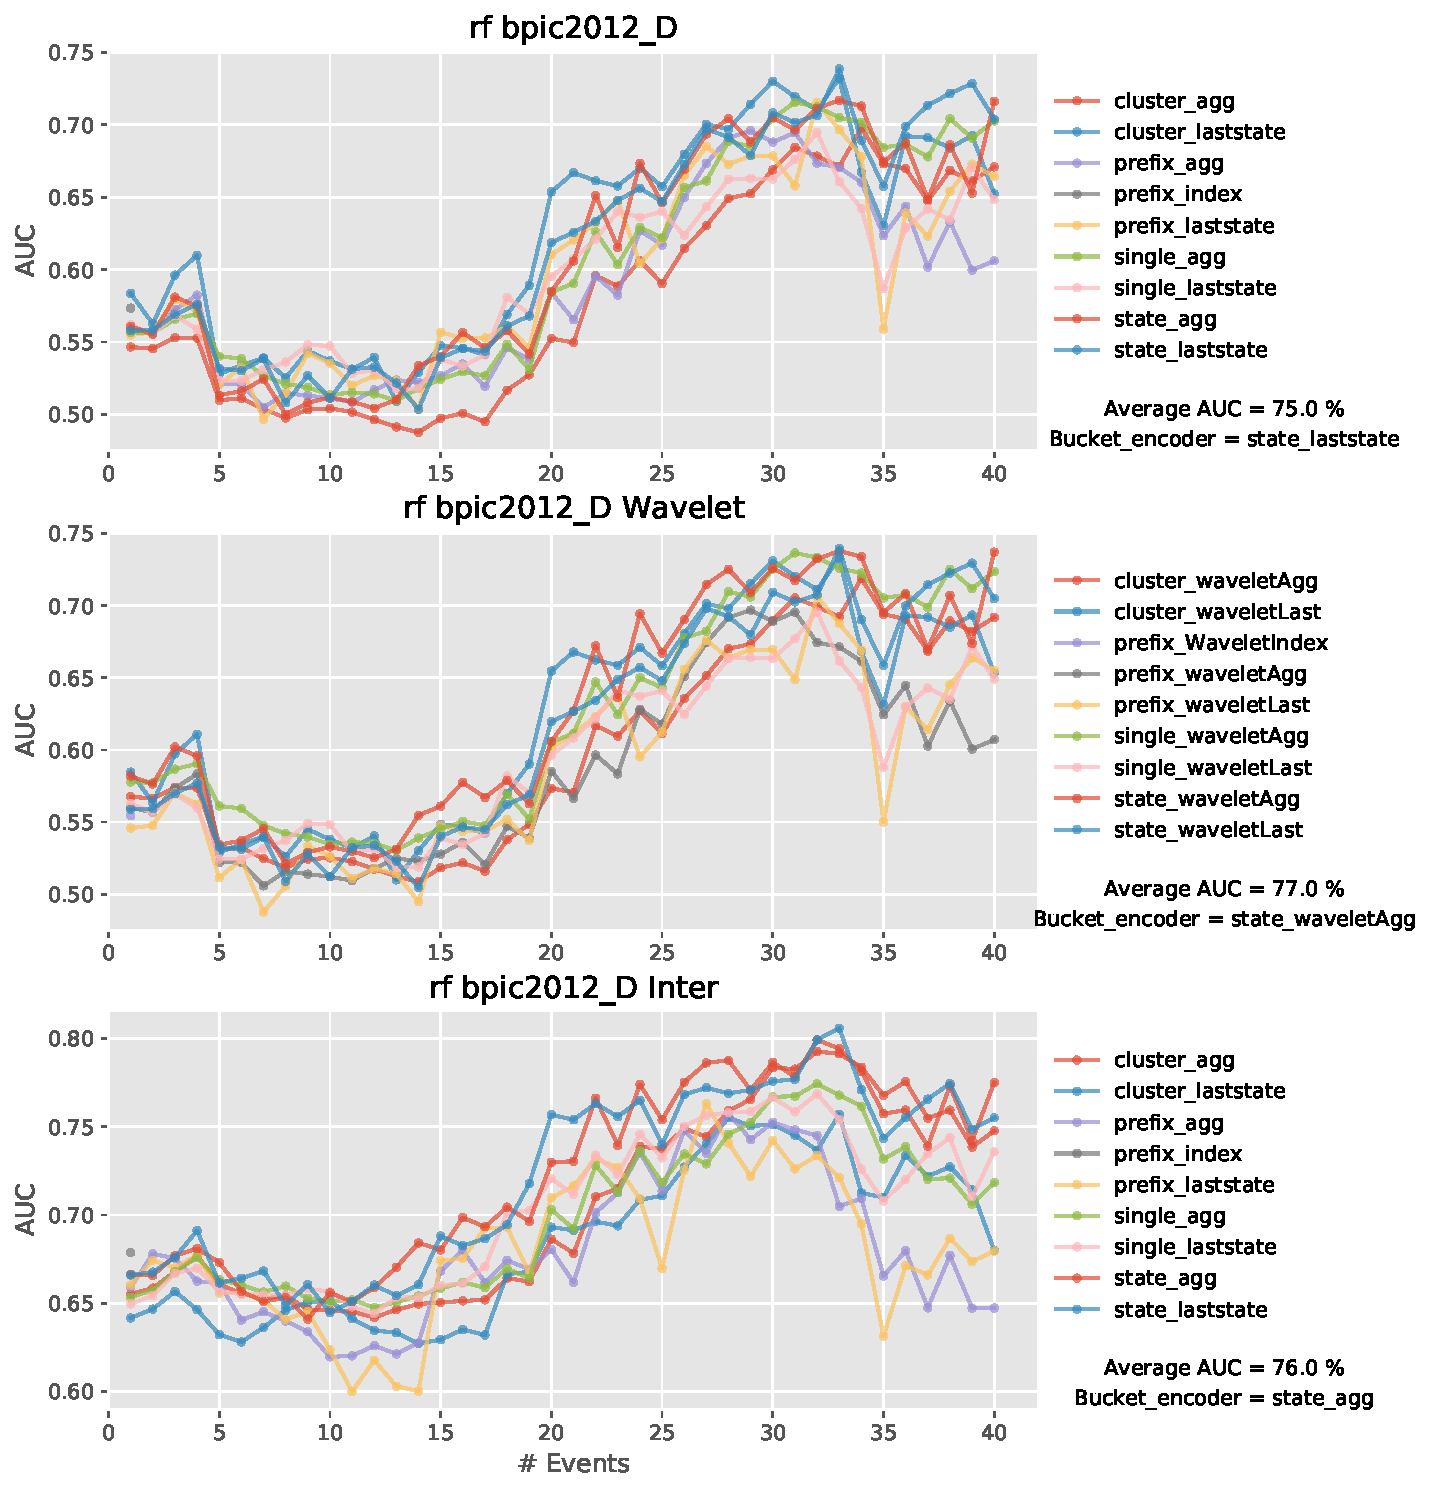
\includegraphics[width=\linewidth]{images/inter/rf/bpic2012_D.pdf}
		\caption{Bpic2012\_D} \label{fig:b12di}
	\end{subfigure}\hspace*{\fill}
	\begin{subfigure}{0.48\textwidth}
		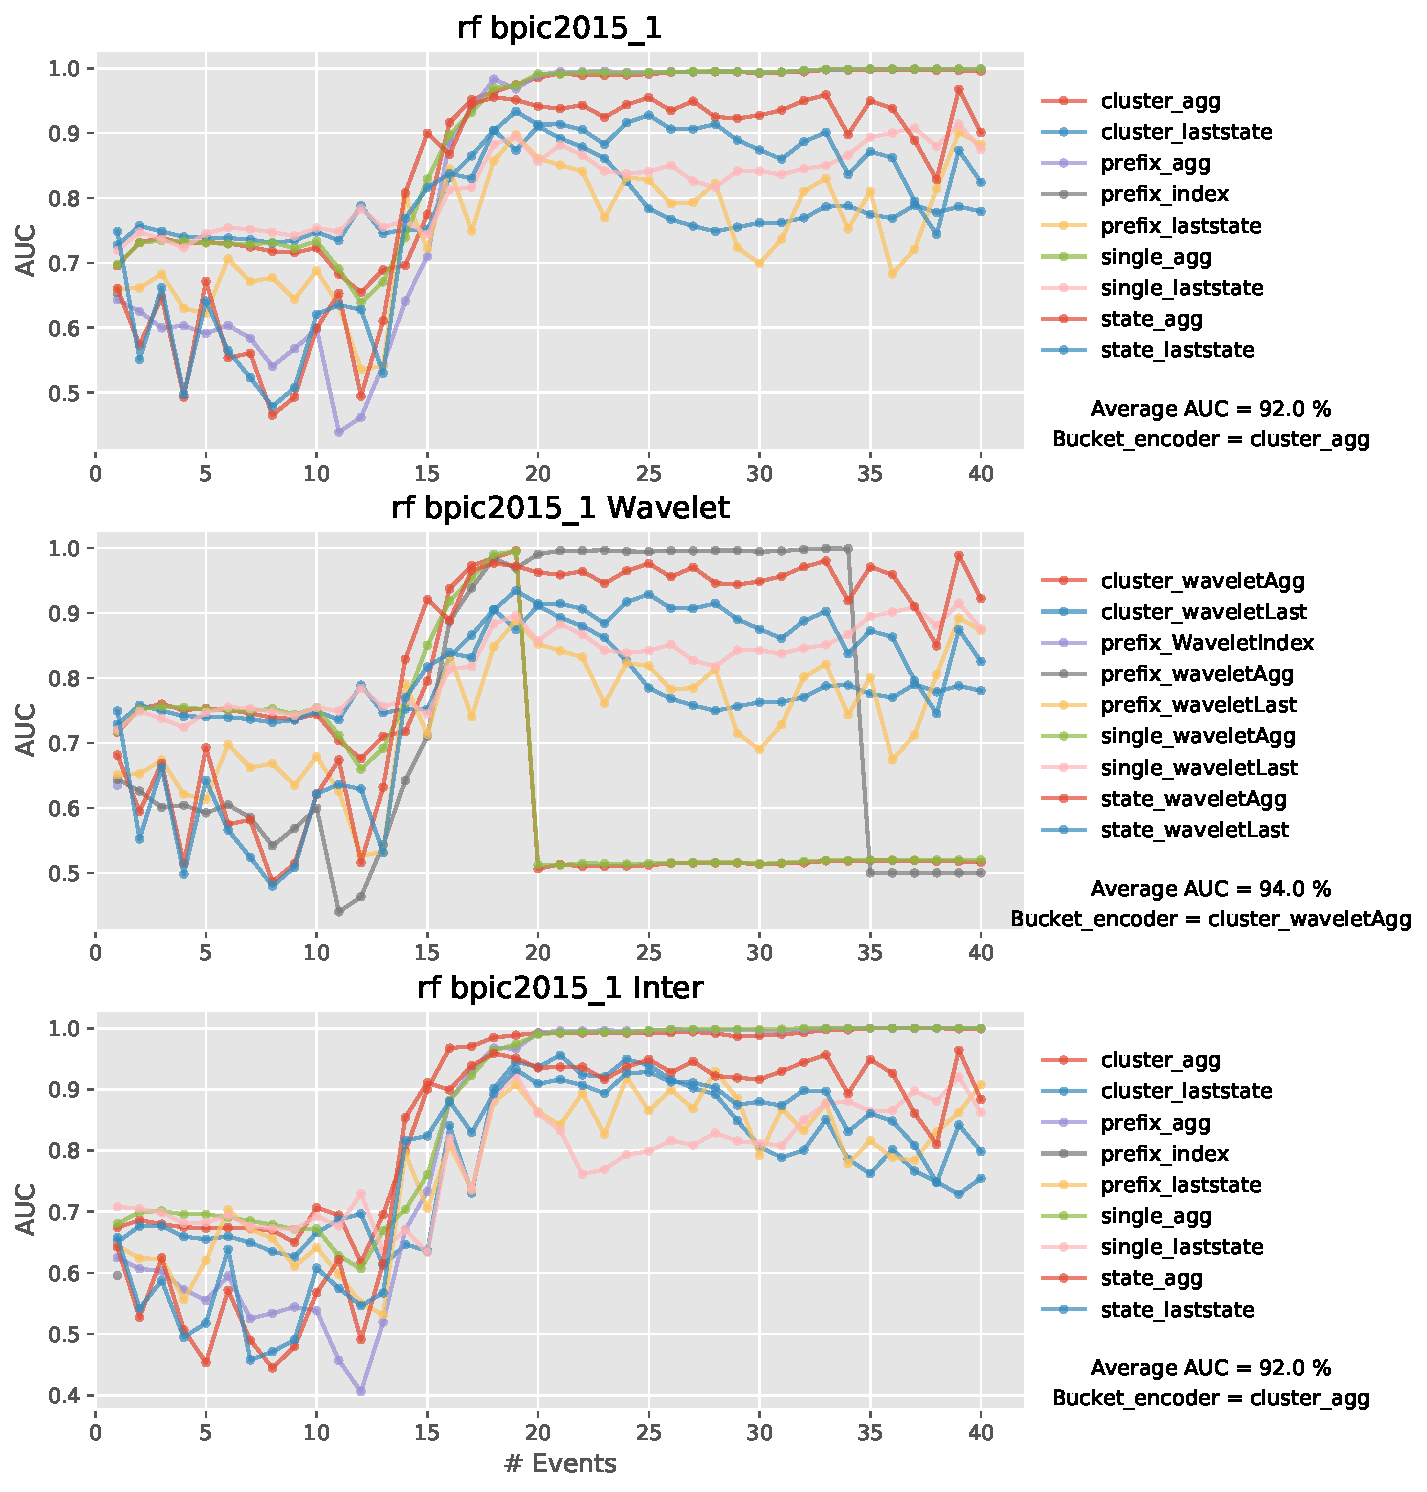
\includegraphics[width=\linewidth]{images/inter/rf/bpic2015_1.pdf}
		\caption{Bpic2015} \label{fig:b151i}
	\end{subfigure}
	
	\begin{subfigure}{0.48\textwidth}
		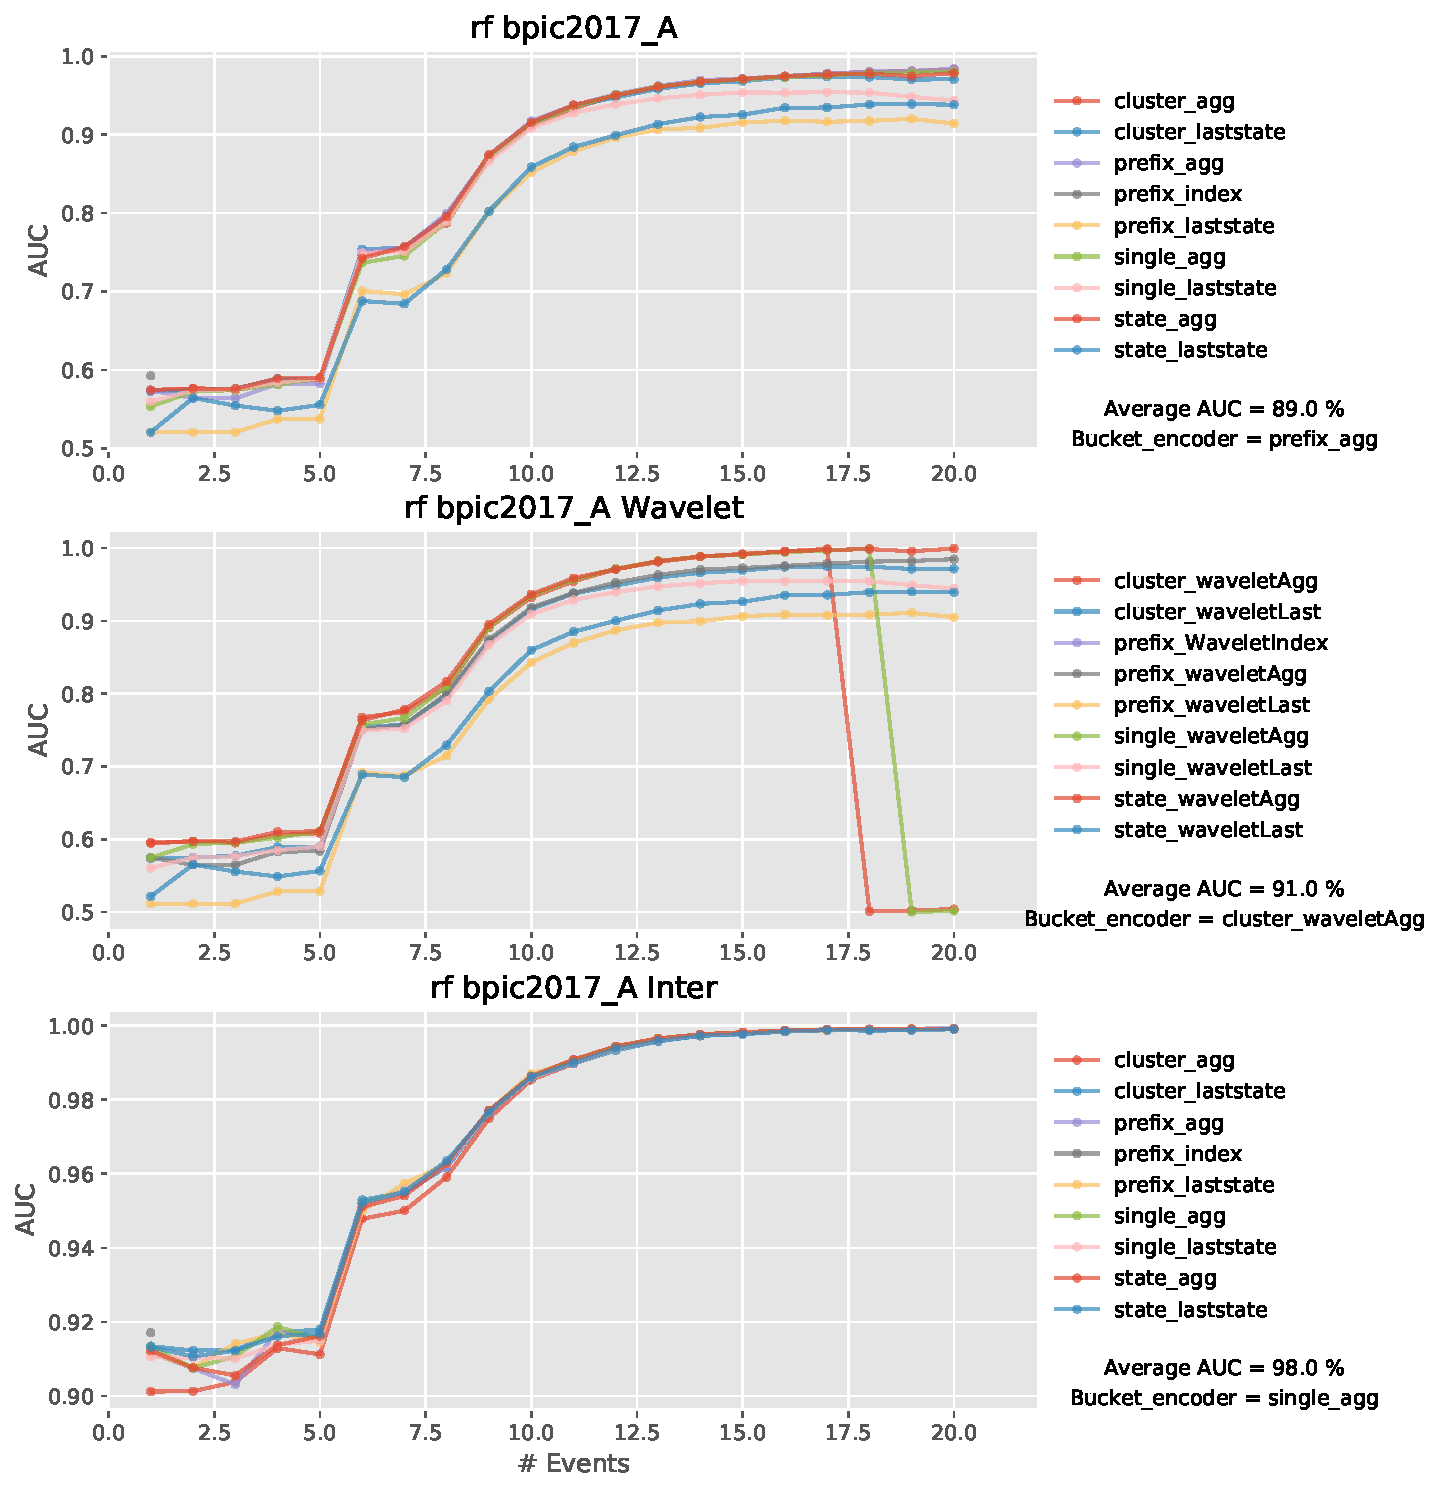
\includegraphics[width=\linewidth]{images/inter/rf/bpic2017_A.pdf}
		\caption{Bpic2017\_A} \label{fig:b17ai}
	\end{subfigure}\hspace*{\fill}
	\begin{subfigure}{0.48\textwidth}
		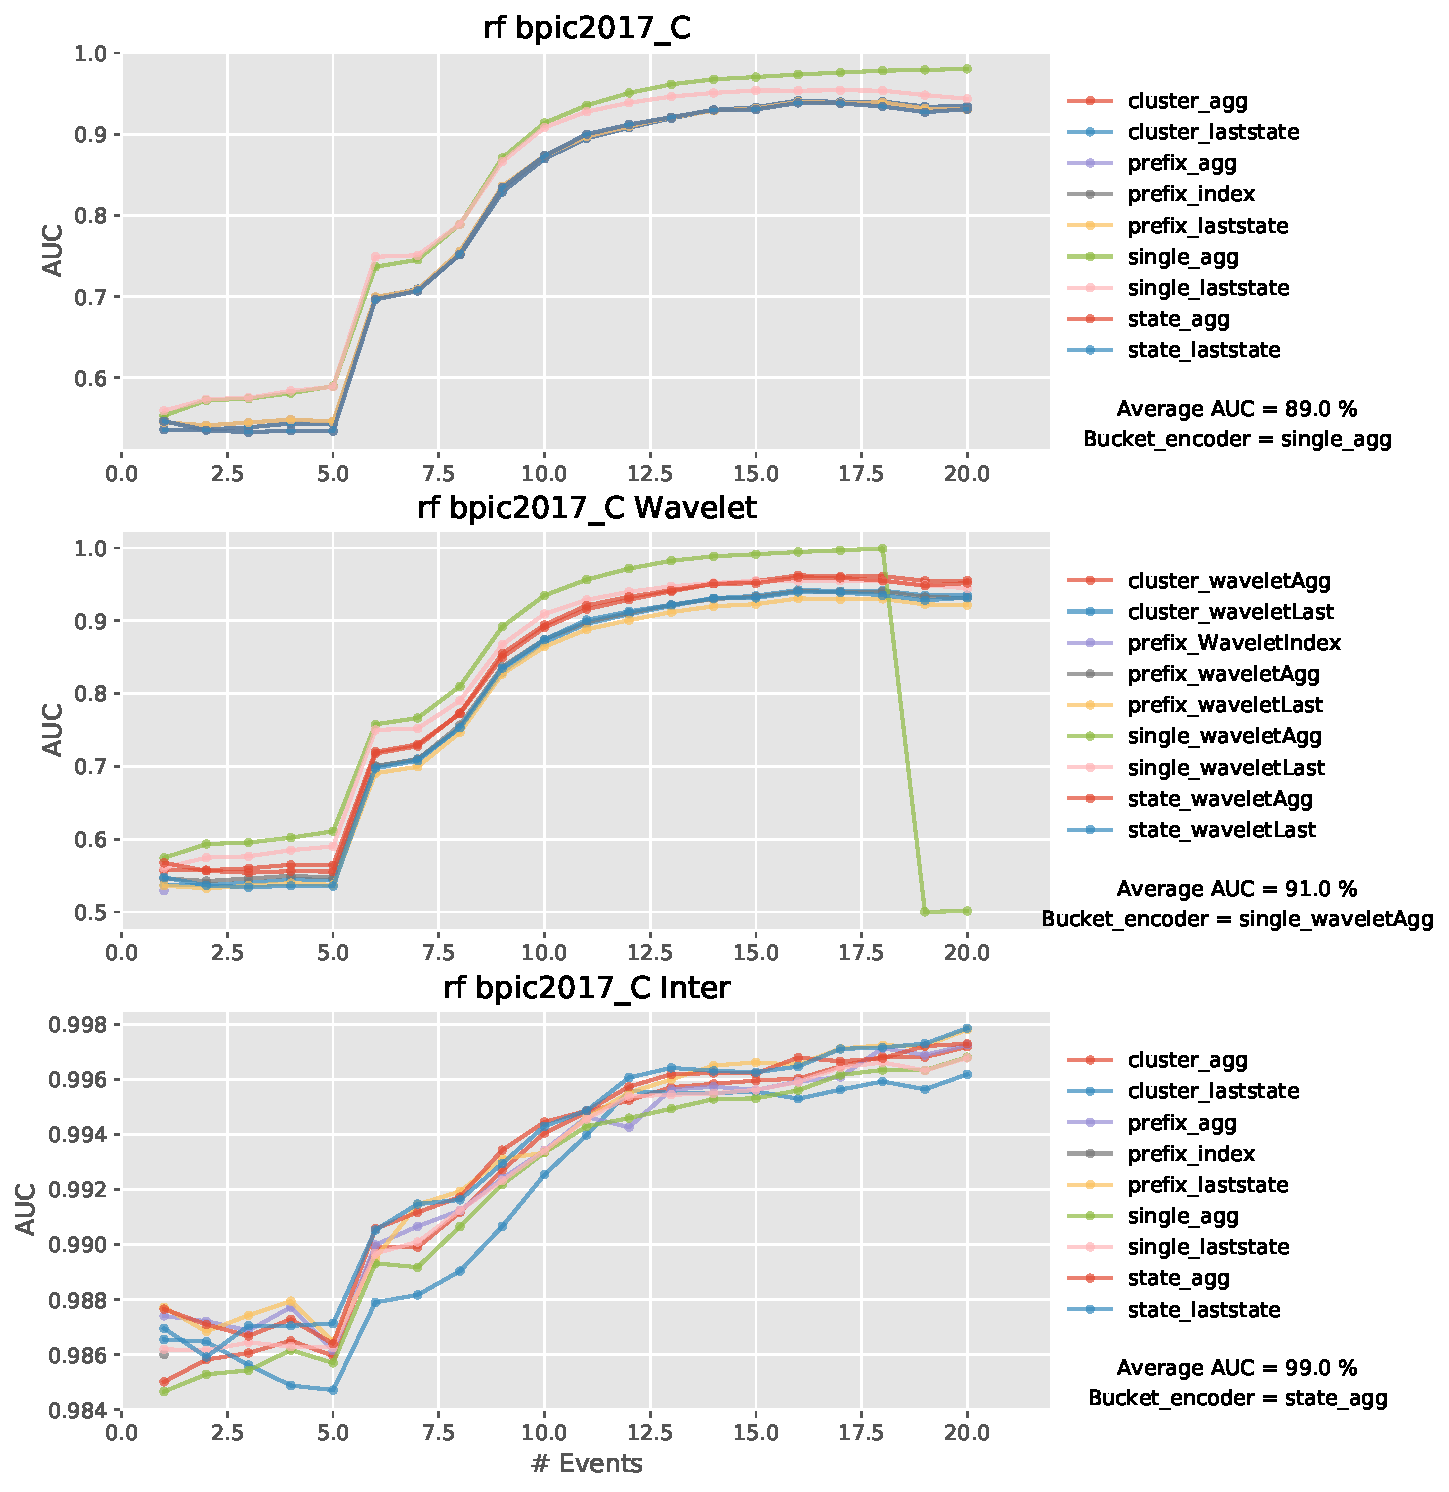
\includegraphics[width=\linewidth]{images/inter/rf/bpic2017_C.pdf}
		\caption{Bpic2017\_C} \label{fig:b17ci}
	\end{subfigure}
		\caption{Comparing RF before and after adding Inter-case features on all event logs}
	\label{fig:interr1}
\end{figure}


\begin{figure}[!htbp] % "[t!]" placement specifier just for this example
	
	\begin{subfigure}{0.48\textwidth}
		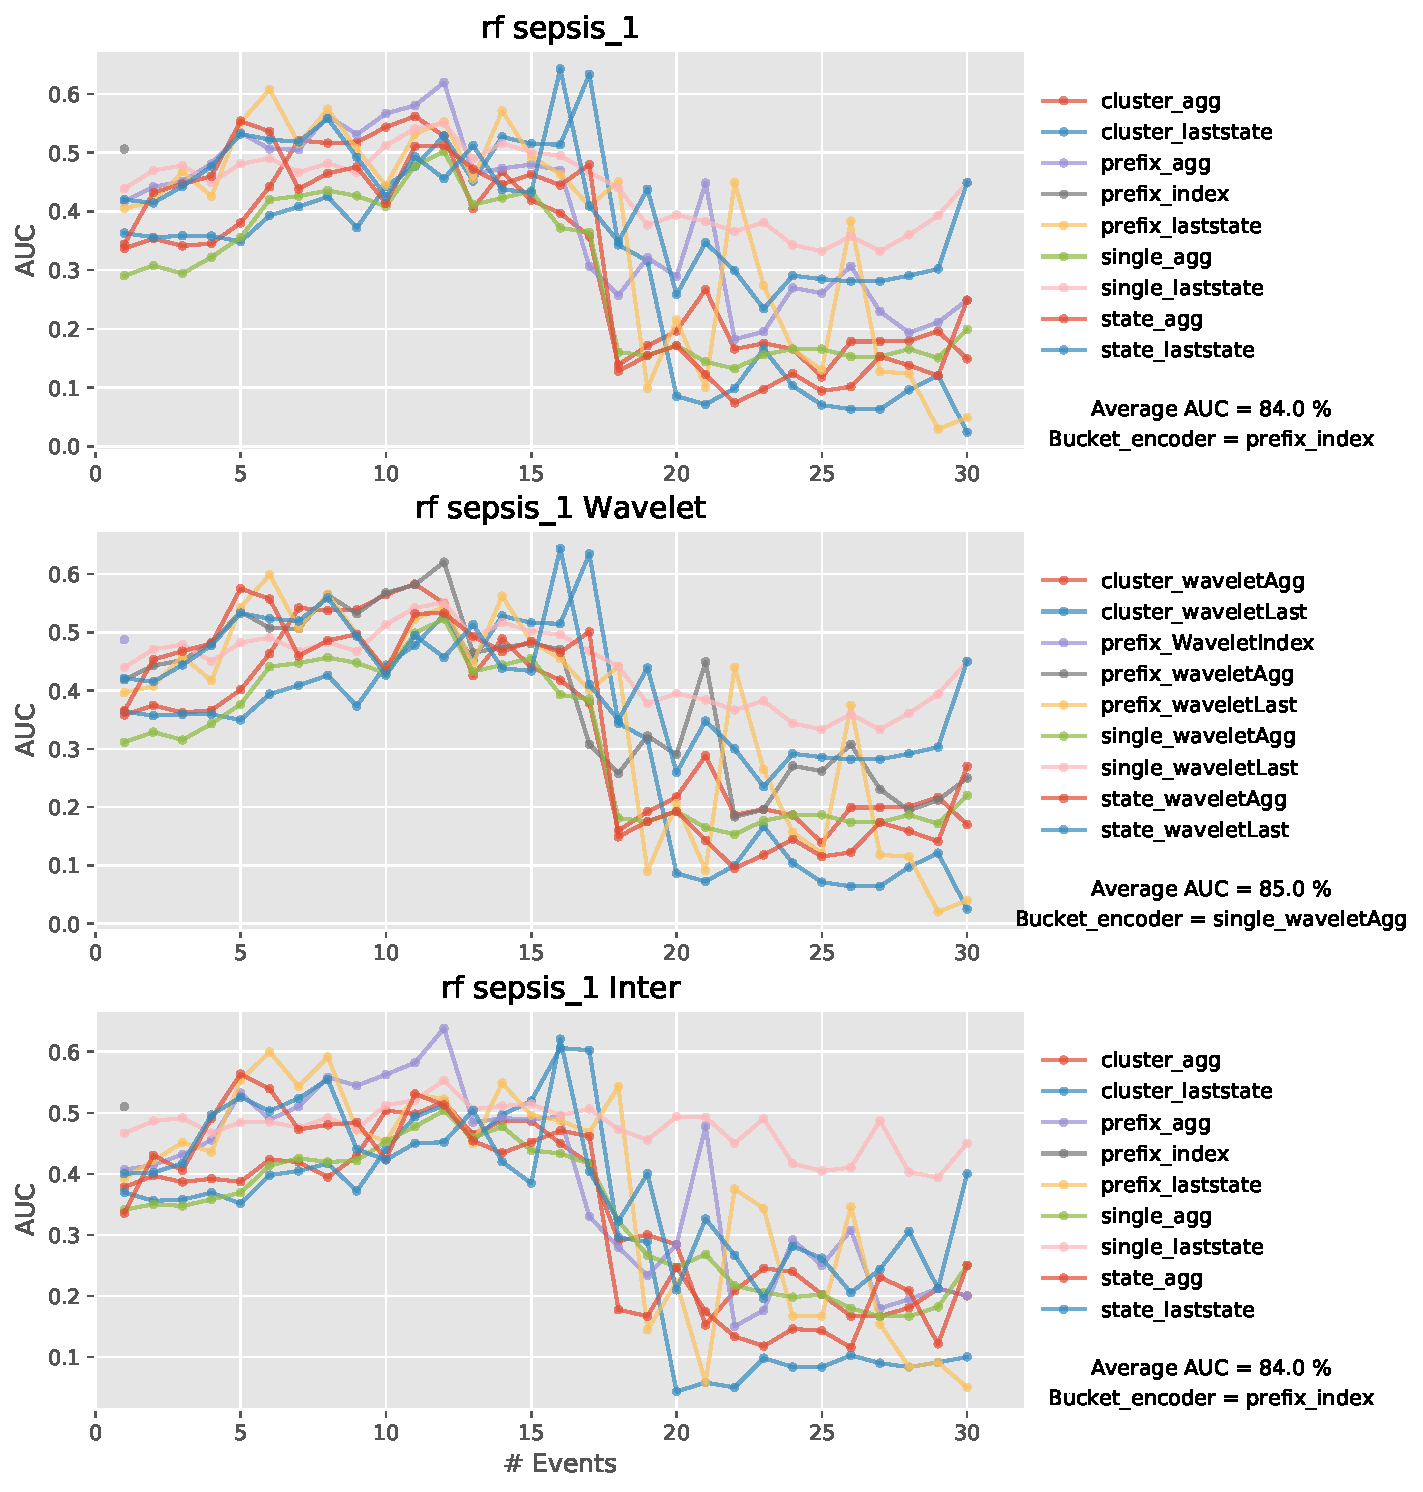
\includegraphics[width=\linewidth]{images/inter/rf/sepsis_1.pdf}
			
			%wavelet/graphs2/sepsis_1.pdf}=
		\caption{Sepsis\_1} \label{fig:sepsisi}
	\end{subfigure}\hspace*{\fill}
	\begin{subfigure}{0.48\textwidth}
		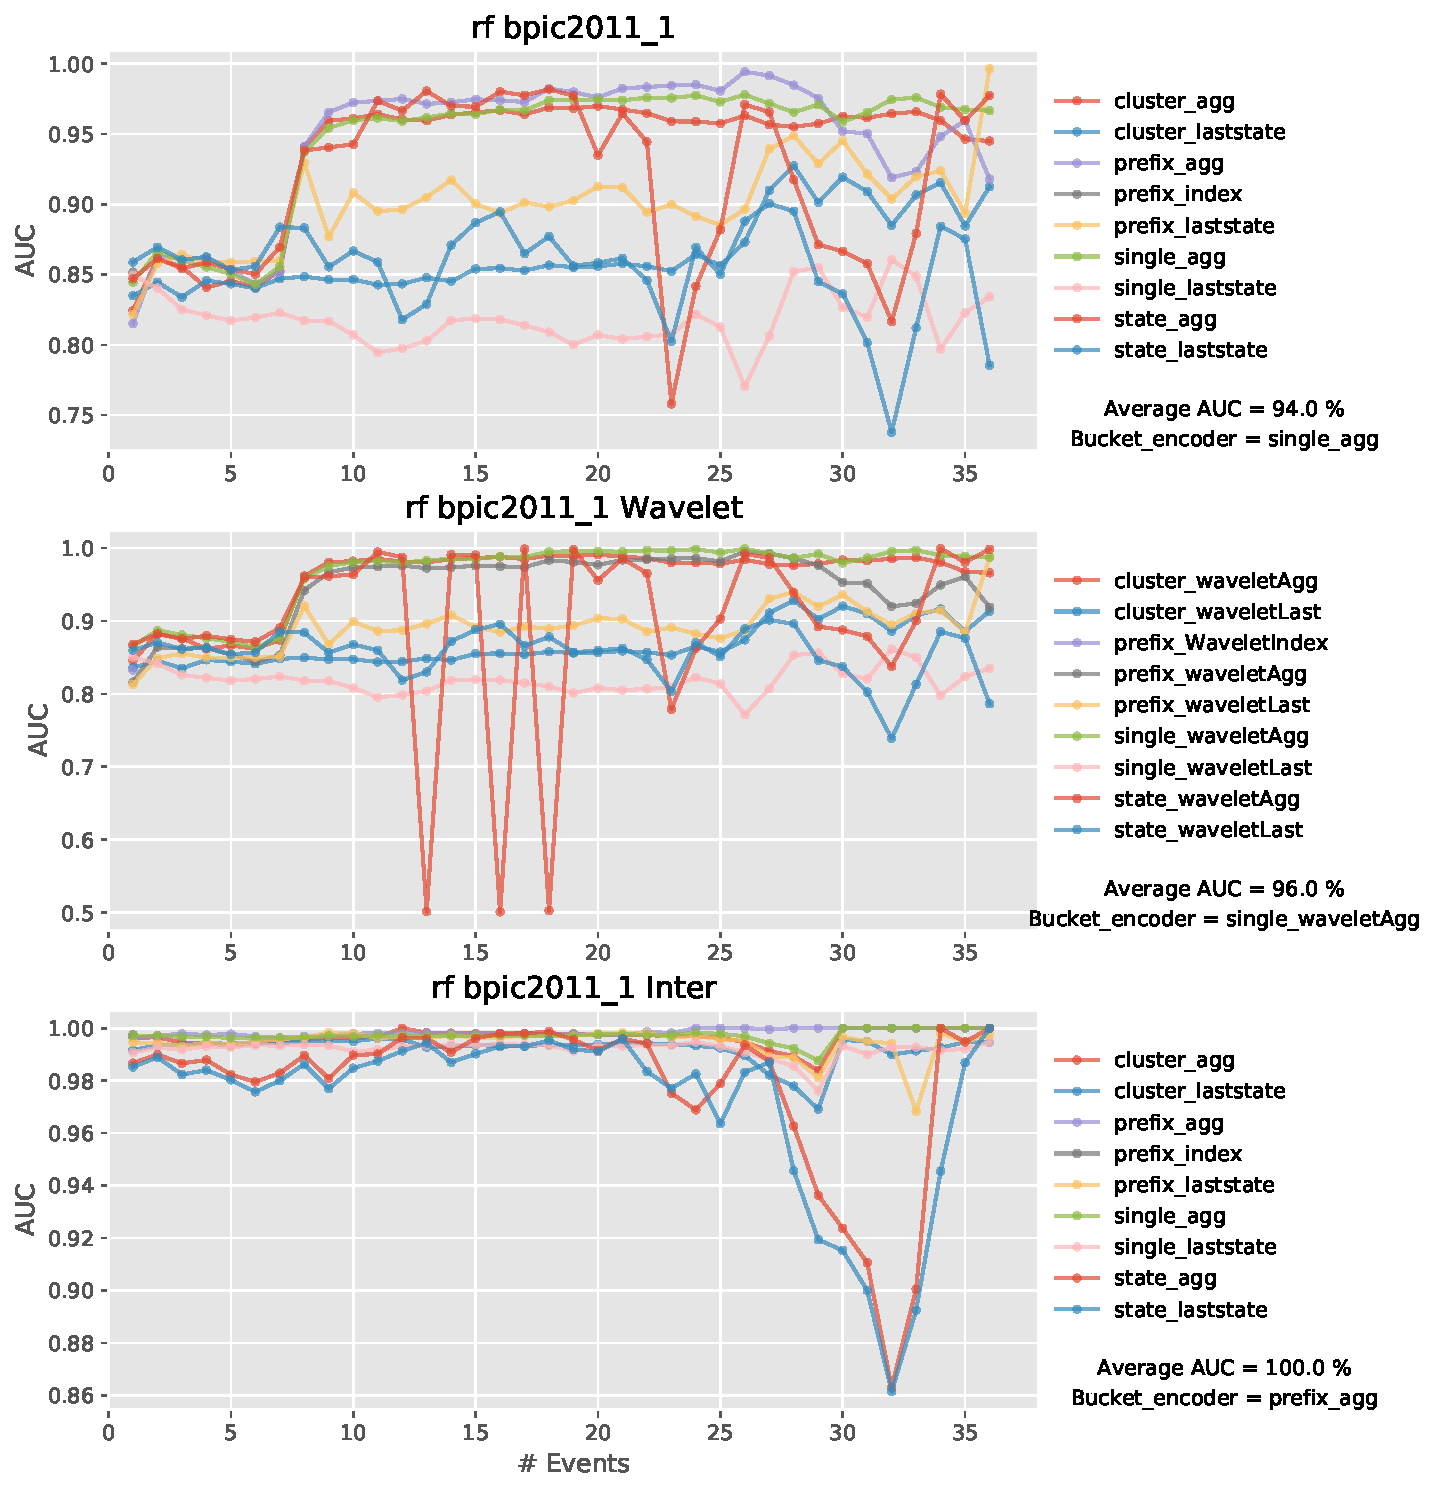
\includegraphics[width=\linewidth]{images/inter/rf/bpic2011_1.pdf}
		\caption{Bpic2011} \label{fig:b11i}
	\end{subfigure}
	
	\medskip
	\begin{subfigure}{0.48\textwidth}
		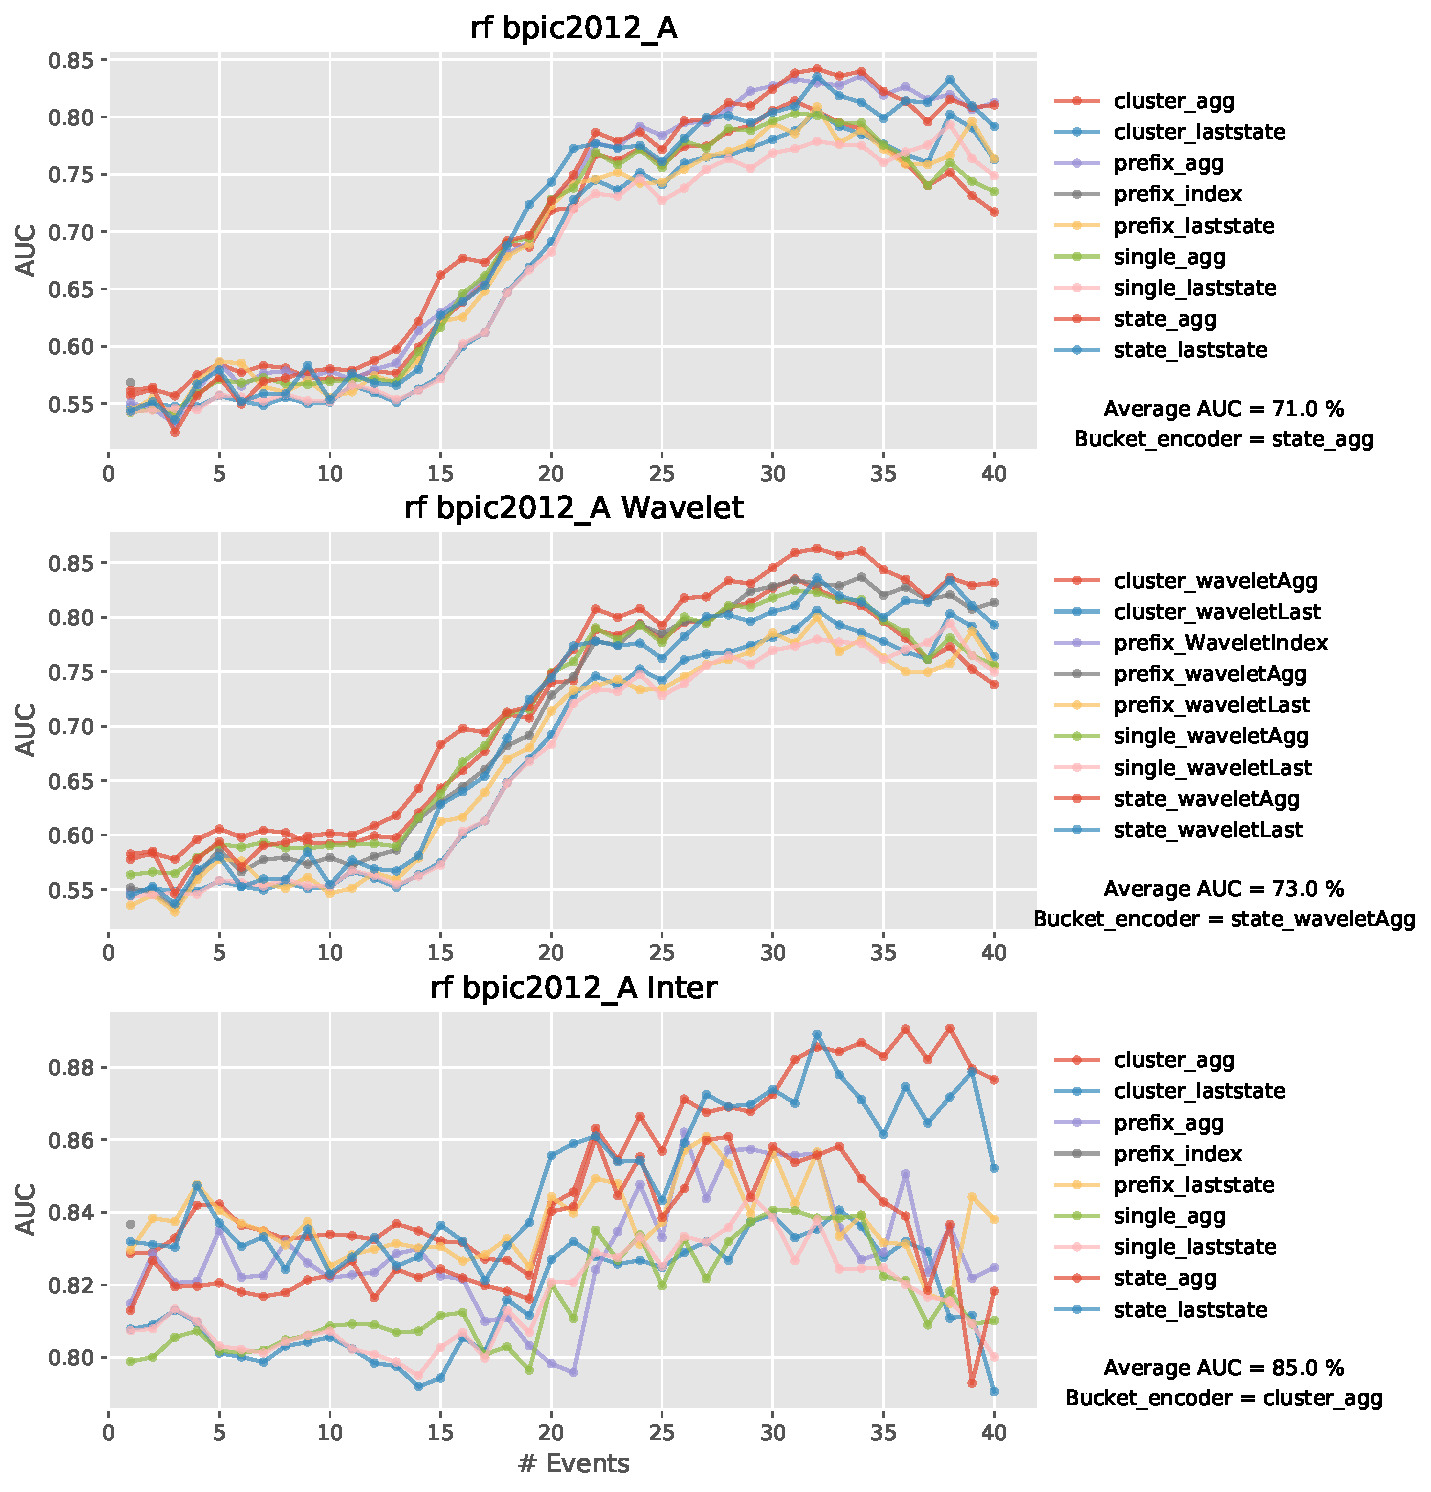
\includegraphics[width=\linewidth]{images/inter/rf/bpic2012_A.pdf}
		\caption{Bpic2012\_A} \label{fig:b12ai}
	\end{subfigure}\hspace*{\fill}
	\begin{subfigure}{0.48\textwidth}
		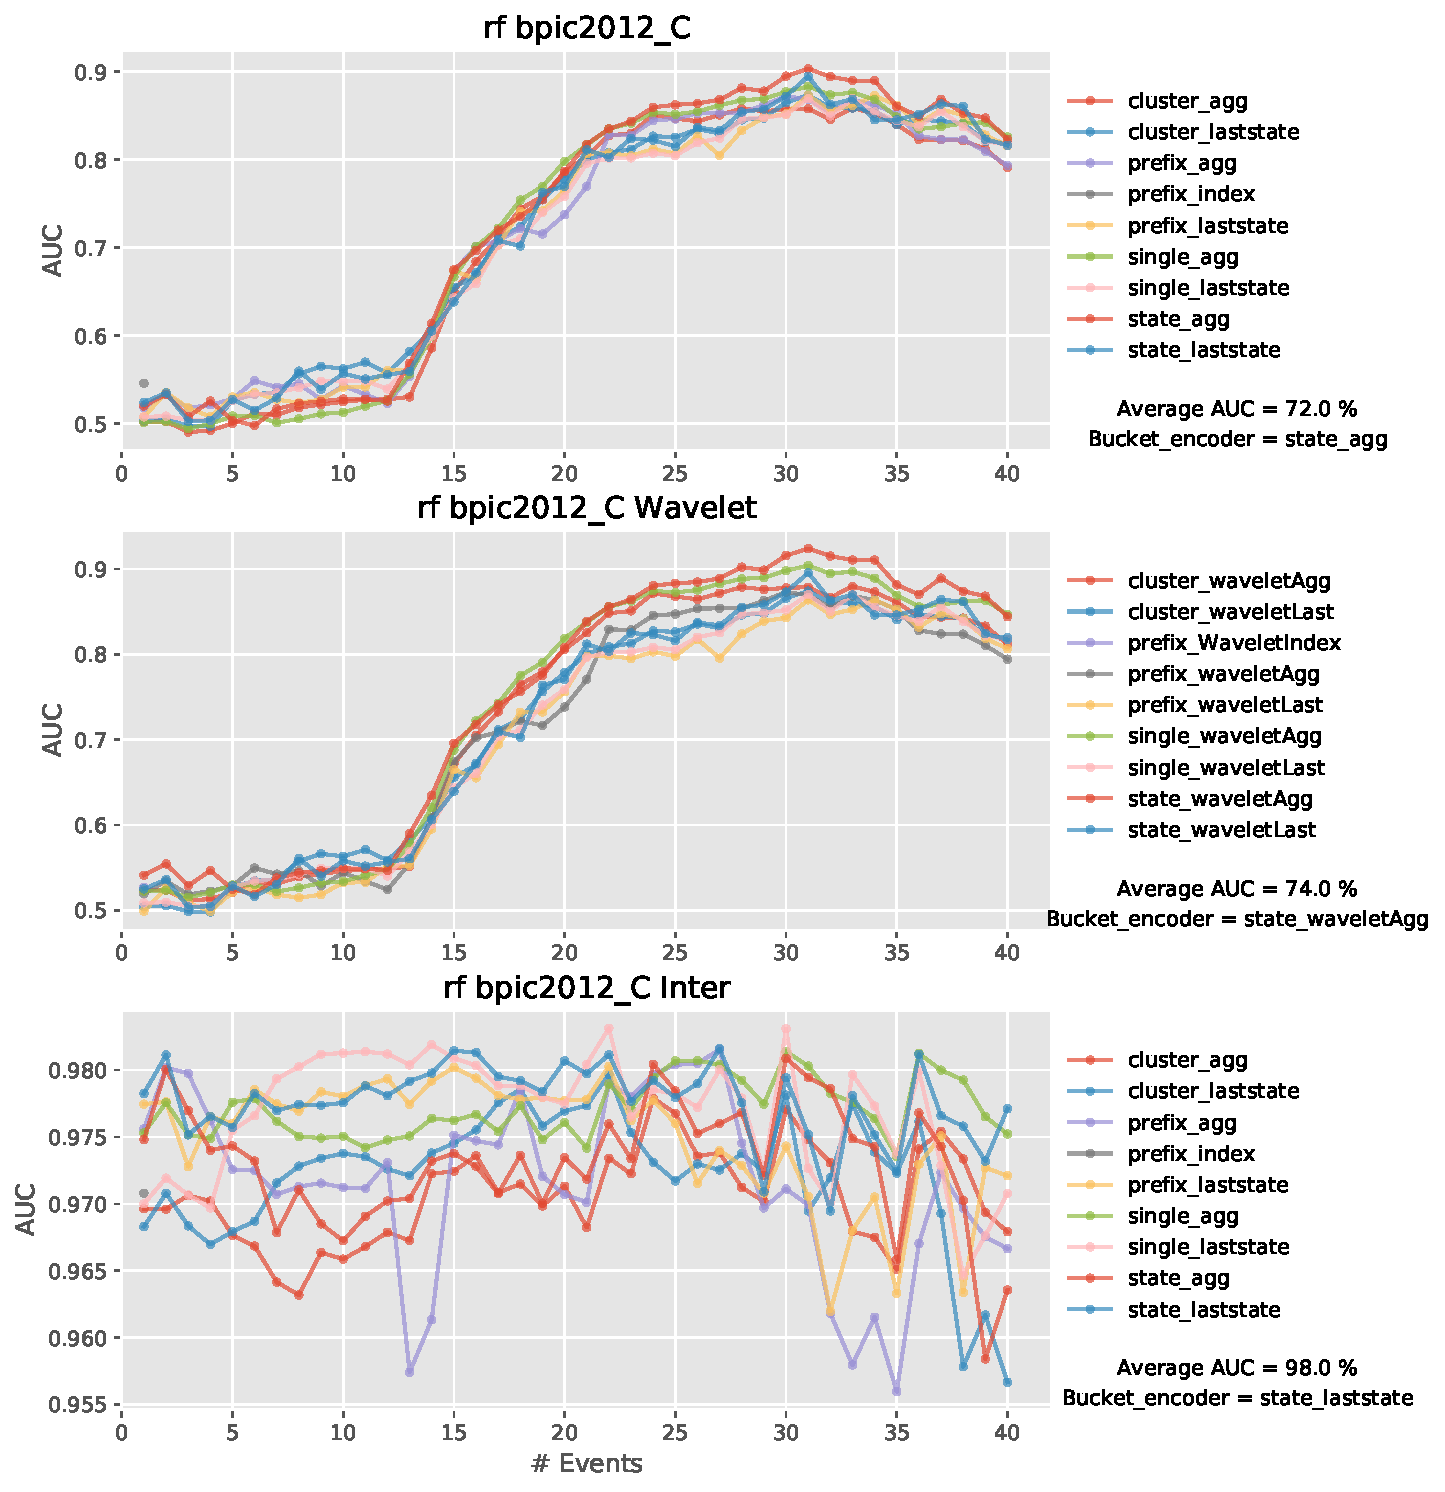
\includegraphics[width=\linewidth]{images/inter/rf/bpic2012_C.pdf}
		\caption{Bpic2012\_C} \label{fig:b12ci}
	\end{subfigure}	
\caption{Comparing RF before and after adding Inter-case features on all event logs  (\textit{continued}).}
\label{fig:interr2}
\end{figure}





\begin{figure}[!htbp] % "[t!]" placement specifier just for this example

	\begin{subfigure}{0.48\textwidth}
		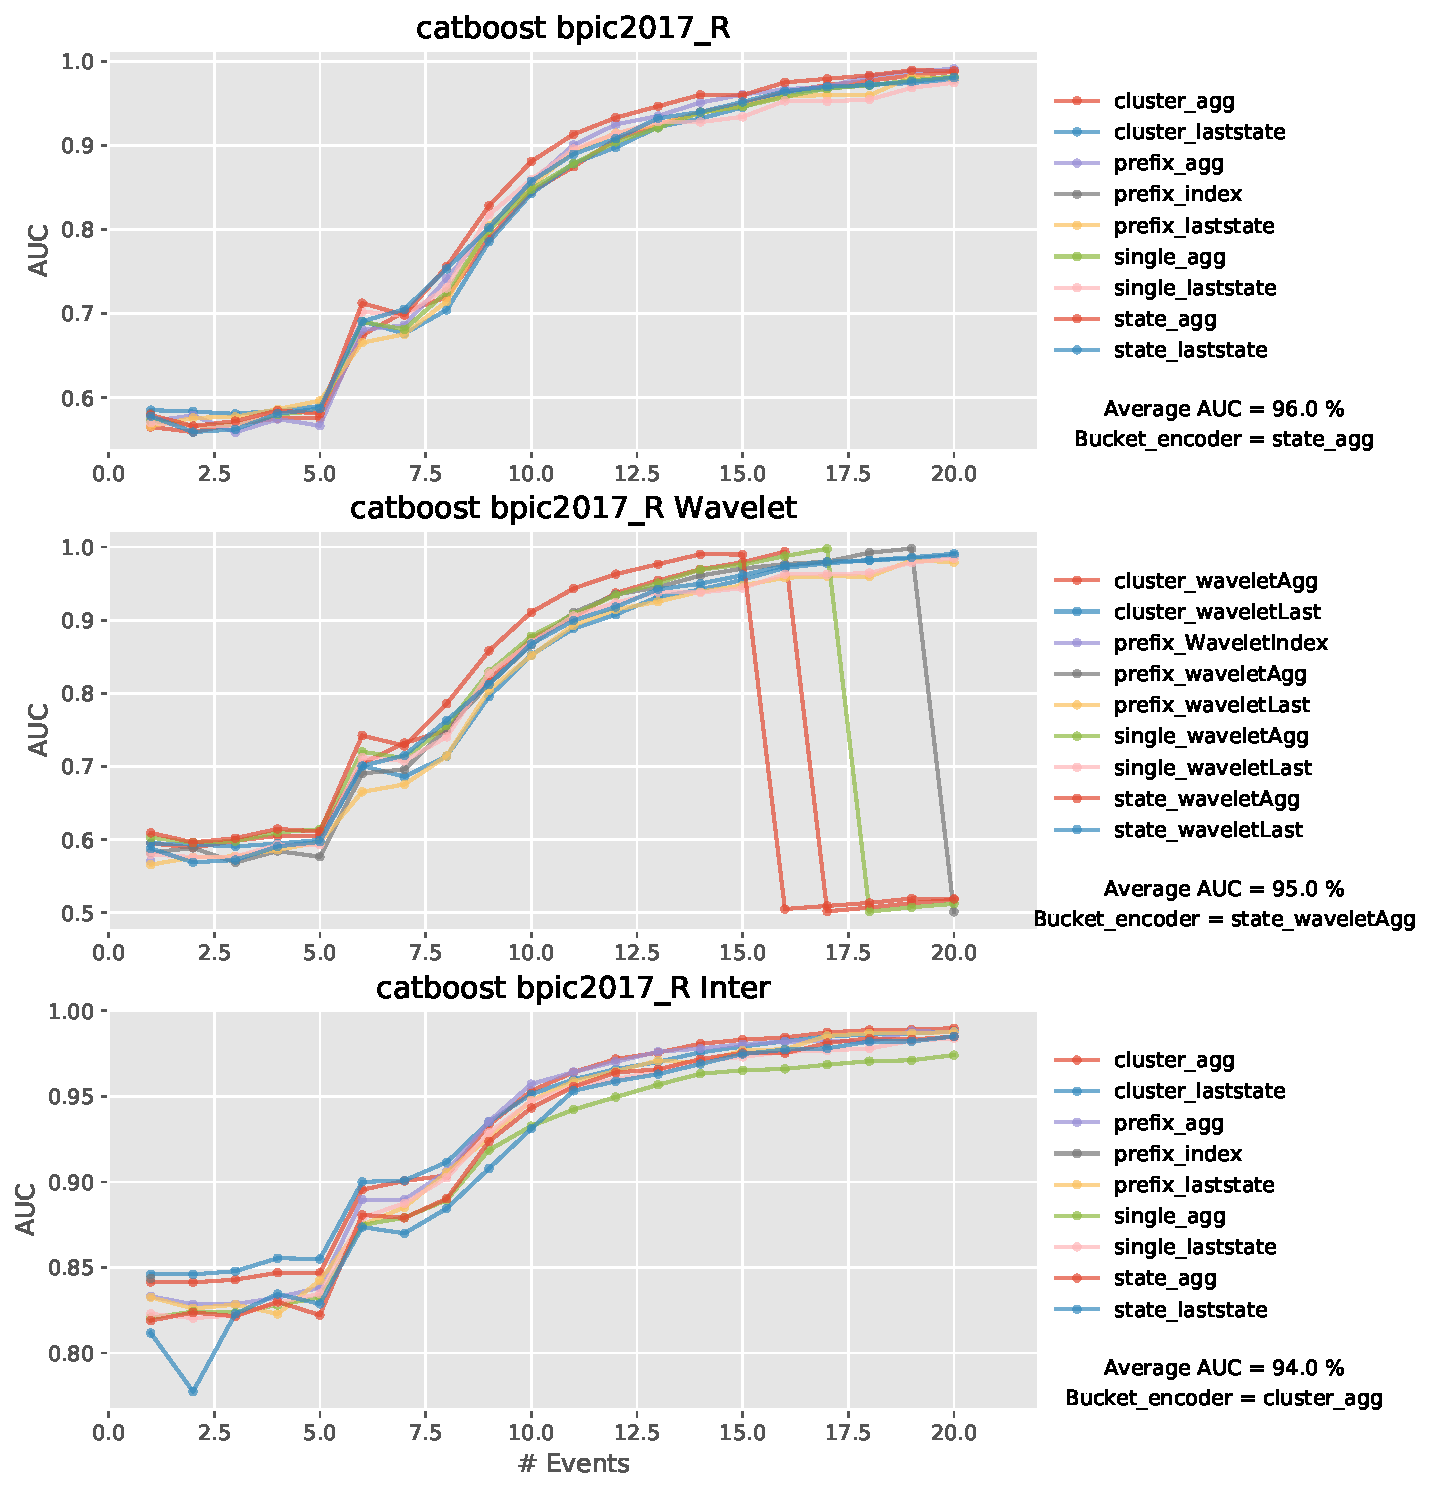
\includegraphics[width=\linewidth]{images/inter/catboost/bpic2017_R.pdf}
		\caption{Wavelet bpic2017\_R} \label{fig:b17ri}
	\end{subfigure}\hspace*{\fill}
	\begin{subfigure}{0.48\textwidth}
		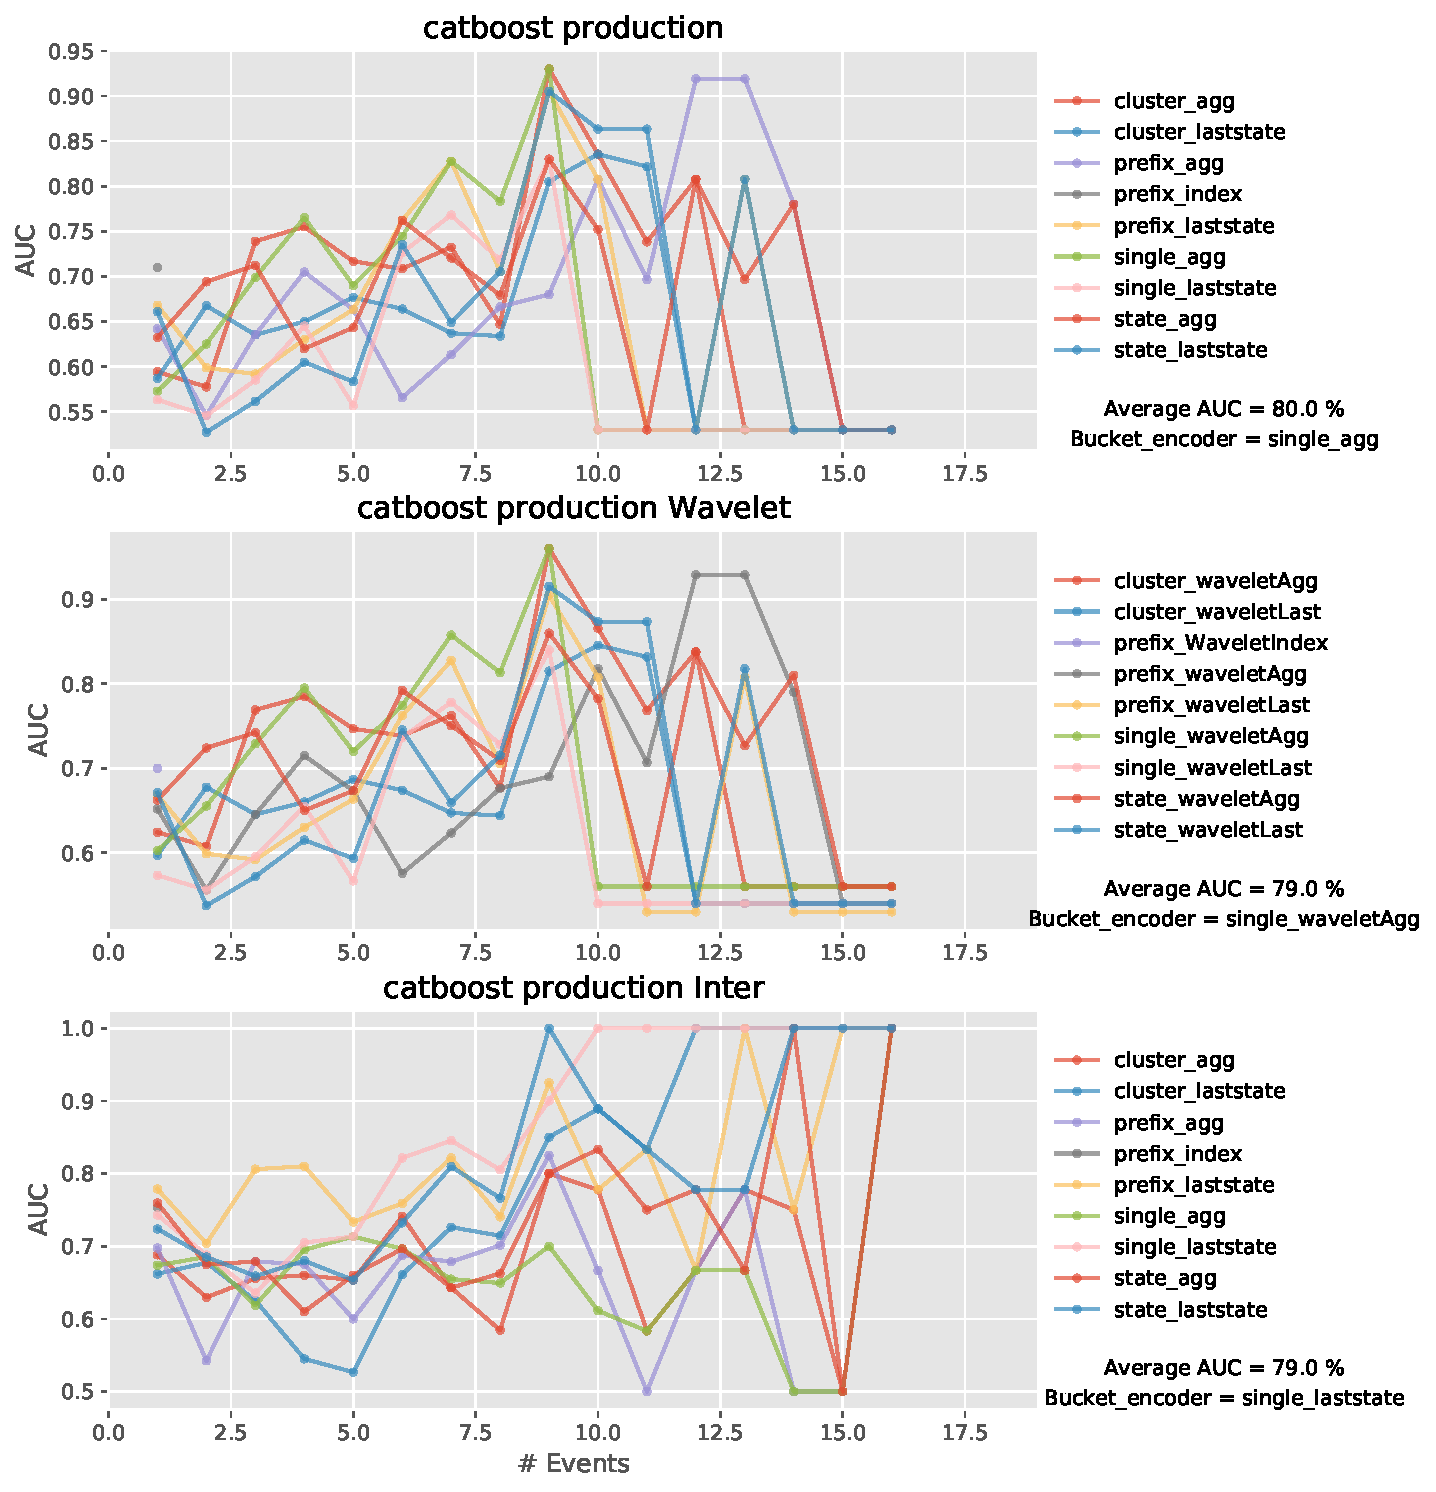
\includegraphics[width=\linewidth]{images/inter/catboost/production.pdf}
		\caption{Production} \label{fig:proi}
	\end{subfigure}\hspace*{\fill}
	\caption{Comparing RF before and after adding Inter-case features on all event logs (\textit{continued})}
\label{fig:interr3}
\end{figure}


\clearpage
\subsubsection{Inter-case features interpretability}

%##### ADD SHAP VALUE ANALYSIS
After adding inter-case features to our predictive models, we achieved a very good performance in terms of accuracy, which leads us to analyze and understand how and why our model achieved this jump in performance. To understand the behaviour of our outcome-oriented predictive models after adding inter-case features, we used a consolidated framework (i.e. \textit{SHAP}) to explain how predictions are made using these models. \textit{\textbf{SH}apley \textbf{A}dditive ex\textbf{P}}lanations gives every feature a weight that refers to the importance of this feature for a specific prediction \cite{lundberg2017unified}. Particularly, SHAP values attempt to describe the outcome of a model as a total amount of the effects of every feature being entered into a conditional expectation \cite{lundberg2018consistent}.


In this thesis, we worked with binary classification problems, which means our target label has two possible values $0$ or $1$ (or $\{0,1\}$). SHAP  provides us with a detailed logic about which inter-case features have the highest effect or impact in the model. We used \textit{Production} event log with SHAP analysis. For example, considering the right decision of predicting the number of discarded product orders is less than zero, which represents our \textit{false} or zero outcomes.  Figure \ref{fig:ffp} shows an explanation of features where every one of them contributing to shifting the model outcome from the goal value  (the common model outcome across the training event log we passed) to the original model outcome. Inter-case features forcing the forecast higher are displayed in \textit{red} such as \textit{open\_cases}, and those forcing the forecast lower are in \textit{blue} as \textit{nr\_ongoing\_cases}. This figure is related to only one case from the event log, and the outcome for it is negative or false. On the other hand, for another case from the event log with an actual positive outcome, we can see from figure \ref{fig:tfp} different inter-case features that force the predictive model towards a specific output. 

\begin{figure}[!htbp]
	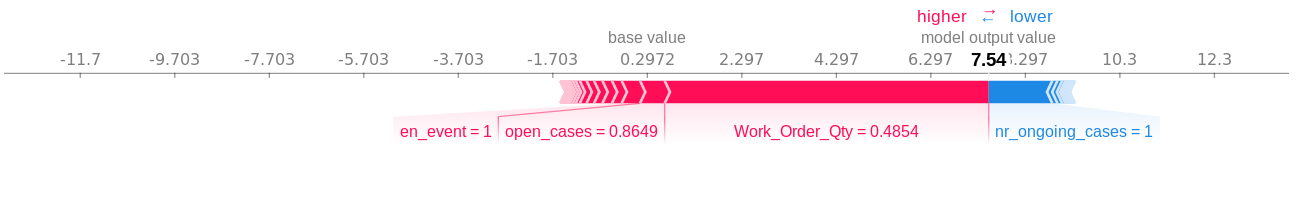
\includegraphics[width=\linewidth]{images/shap/false_force_plot_sc.png}
	\caption[SHAP force plot product (false outcome)]{SHAP value analysis explanation when predicting the number of discarded product orders is less than zero. Features with red colour are pushing model higher for prediction and vice verse with blue.}
	\label{fig:ffp}
\end{figure}\hspace*{\fill}

\begin{figure}[!htbp]
	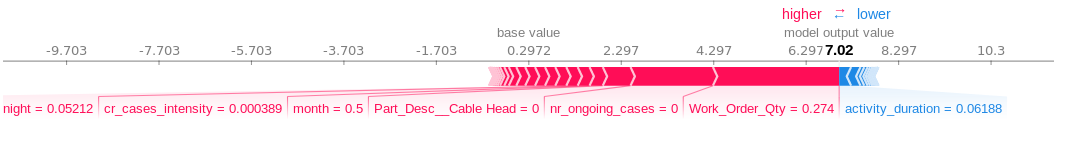
\includegraphics[width=\linewidth]{images/shap/true_fp.png}
	\caption[SHAP force plot product (true outcome)]{SHAP value analysis explanation when predicting the number of discarded product orders is more than zero. Features with red colour are pushing model higher for prediction and vice verse with blue.}
	\label{fig:tfp}
\end{figure}\hspace*{\fill}

Figures \ref{fig:ffp}, and \ref{fig:tfp} both contain an inter-case feature, i.e. \textit{(nr\_ongoing\_cases)},  that we introduced in this thesis which captures information about the workload of business processes (see section \ref{inter}), and this feature is helping and pushing the model toward the correct prediction either for false or negative outcome correctly, so we decided to explore and interpret this inter-case feature more. 

Figure \ref{fig:afp} shows the effect of using \textit{nr\_ongoing\_cases} on different cases form our event log, i.e. around 700 samples. Results show the nr\_ongoing\_cases feature has a high impact on the model outcome either for false or positive cases, as shown in blue and red, respectively. 

\begin{figure}[!htbp]
	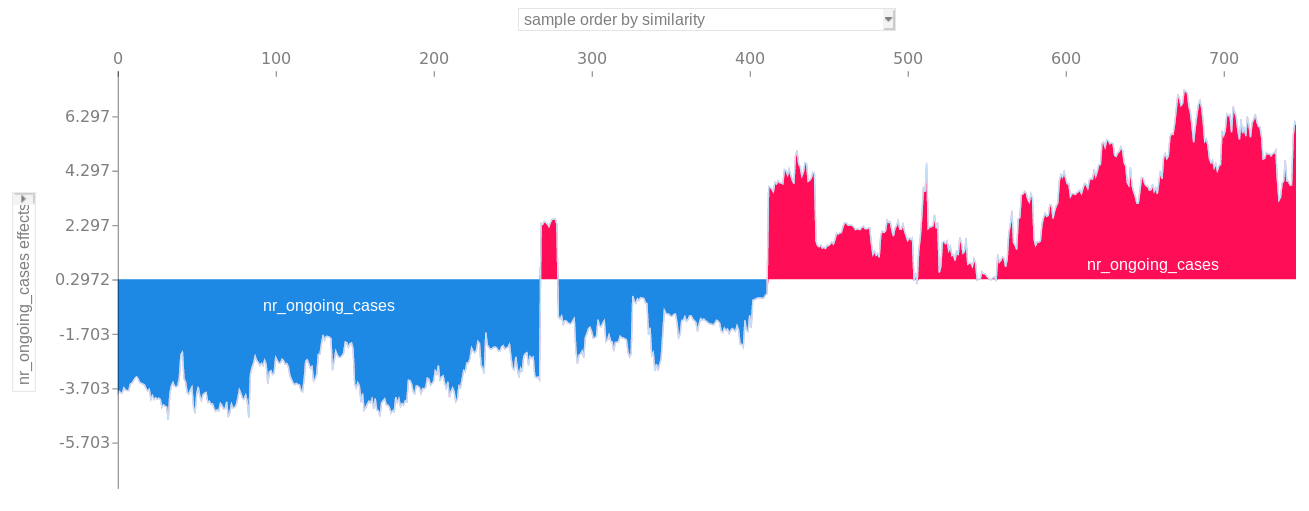
\includegraphics[width=\linewidth]{images/shap/allsamples_ongoing.png}
	\caption[SHAP force plot product (true outcome)]{SHAP value analysis explanation when predicting the number of discarded product orders is more or less than zero in different cases. Features with red colour are pushing model higher for prediction and vice verse with blue.}
	\label{fig:afp}
\end{figure}\hspace*{\fill}


%\begin{figure}[!htbp]
%	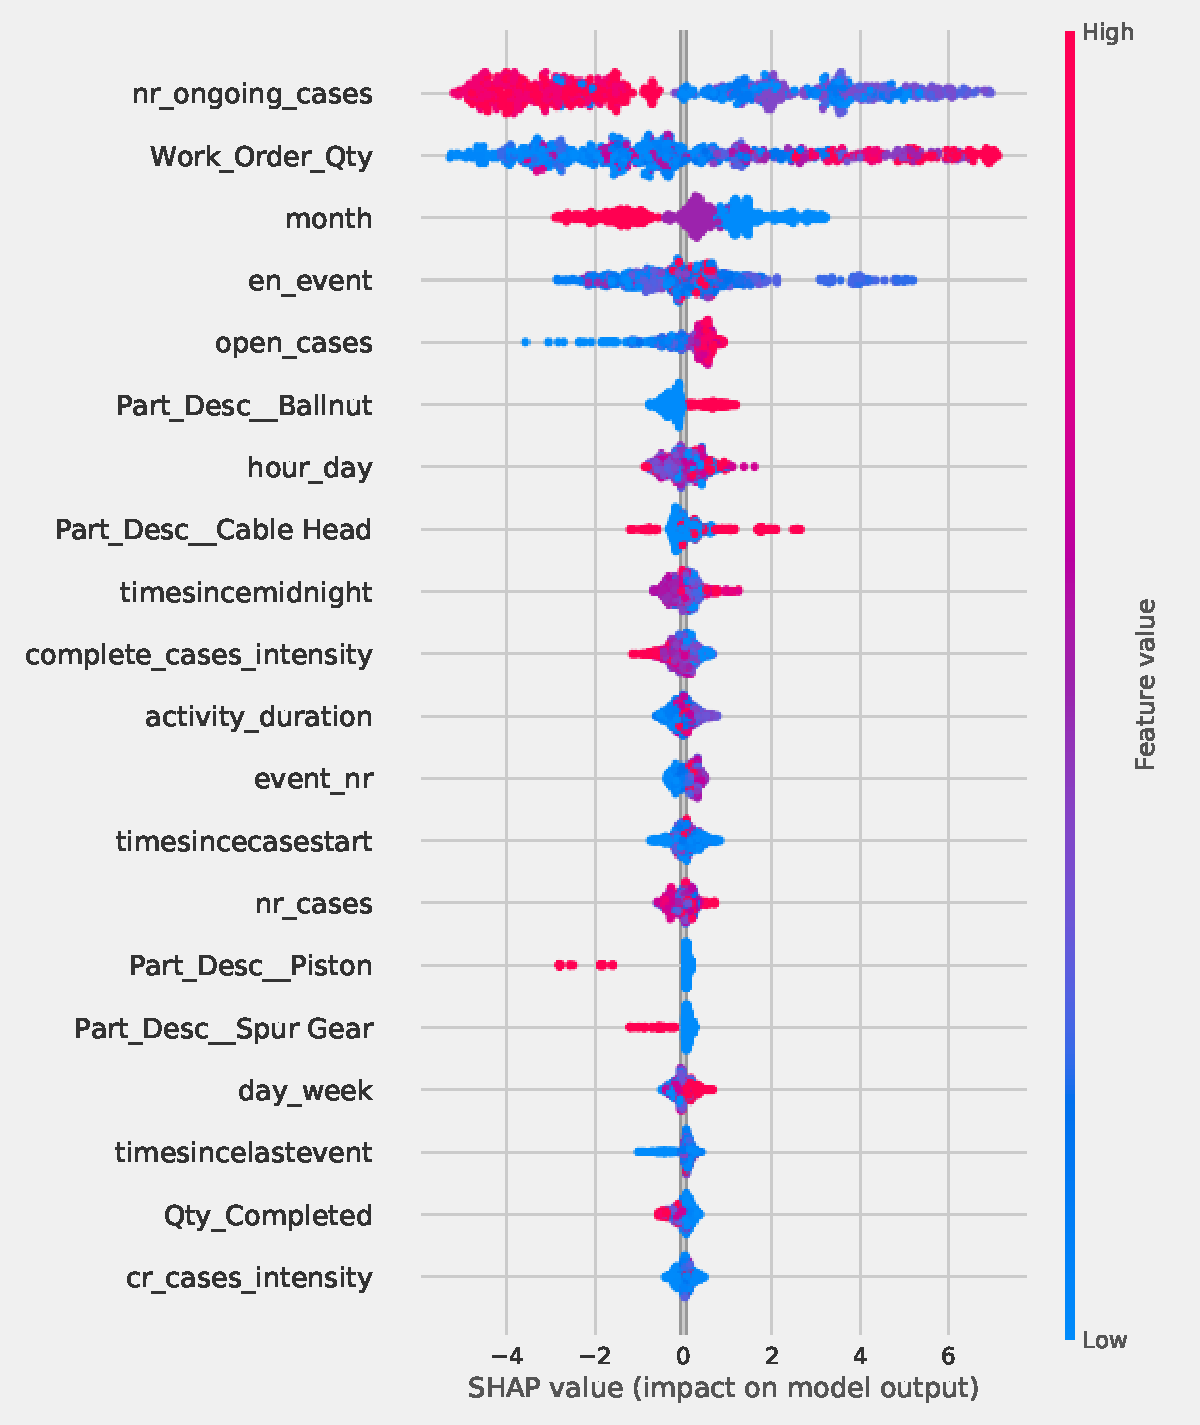
\includegraphics[width=\linewidth]{images/shap/summary_plot.pdf}
%	\caption[SHAP force plot product (true outcome)]{density scatter plot SHAP value analysis explanation when predicting the number of the discarded product orders is more or less than zero on different cases. Features with red color are pushing model higher for prediction and vice verse with blue.}
%	\label{fig:afp}
%\end{figure}\hspace*{\fill}

Figure \ref{fig:SHAP11} shows a traditional bar chart on the basis of the average of the SHAP value measures over the event log and plots it as a simple bar chart. While, figure \ref{fig:shap12}, shows a density scatter plot of SHAP values for every feature to distinguish how much influence every feature has on the model outcome for cases in the validation set. In both figures \ref{fig:shap1}, features are sorted on the basis of the sum of SHAP value measures across overall cases. It is intriguing to remark that one of our introduced inter-case feature that is  \textit{nr\_ongoing\_cases} has a huge impact on the model outcome, and it has the highest SHAP value among all other features. Also, in both figures, we can see three other inter-case features \textit{(i.e. hour\_day, nr\_cases, and cr\_cases\_intensity)} that have a significant SHAP value among all other features in the original event log that reflects on the model output. 


\begin{figure}[!htbp] % "[t!]" placement specifier just for this example
	\caption[SHAP density plot product]{SHAP density plot of}
	\label{fig:shap1}
	\begin{subfigure}{0.48\textwidth}
		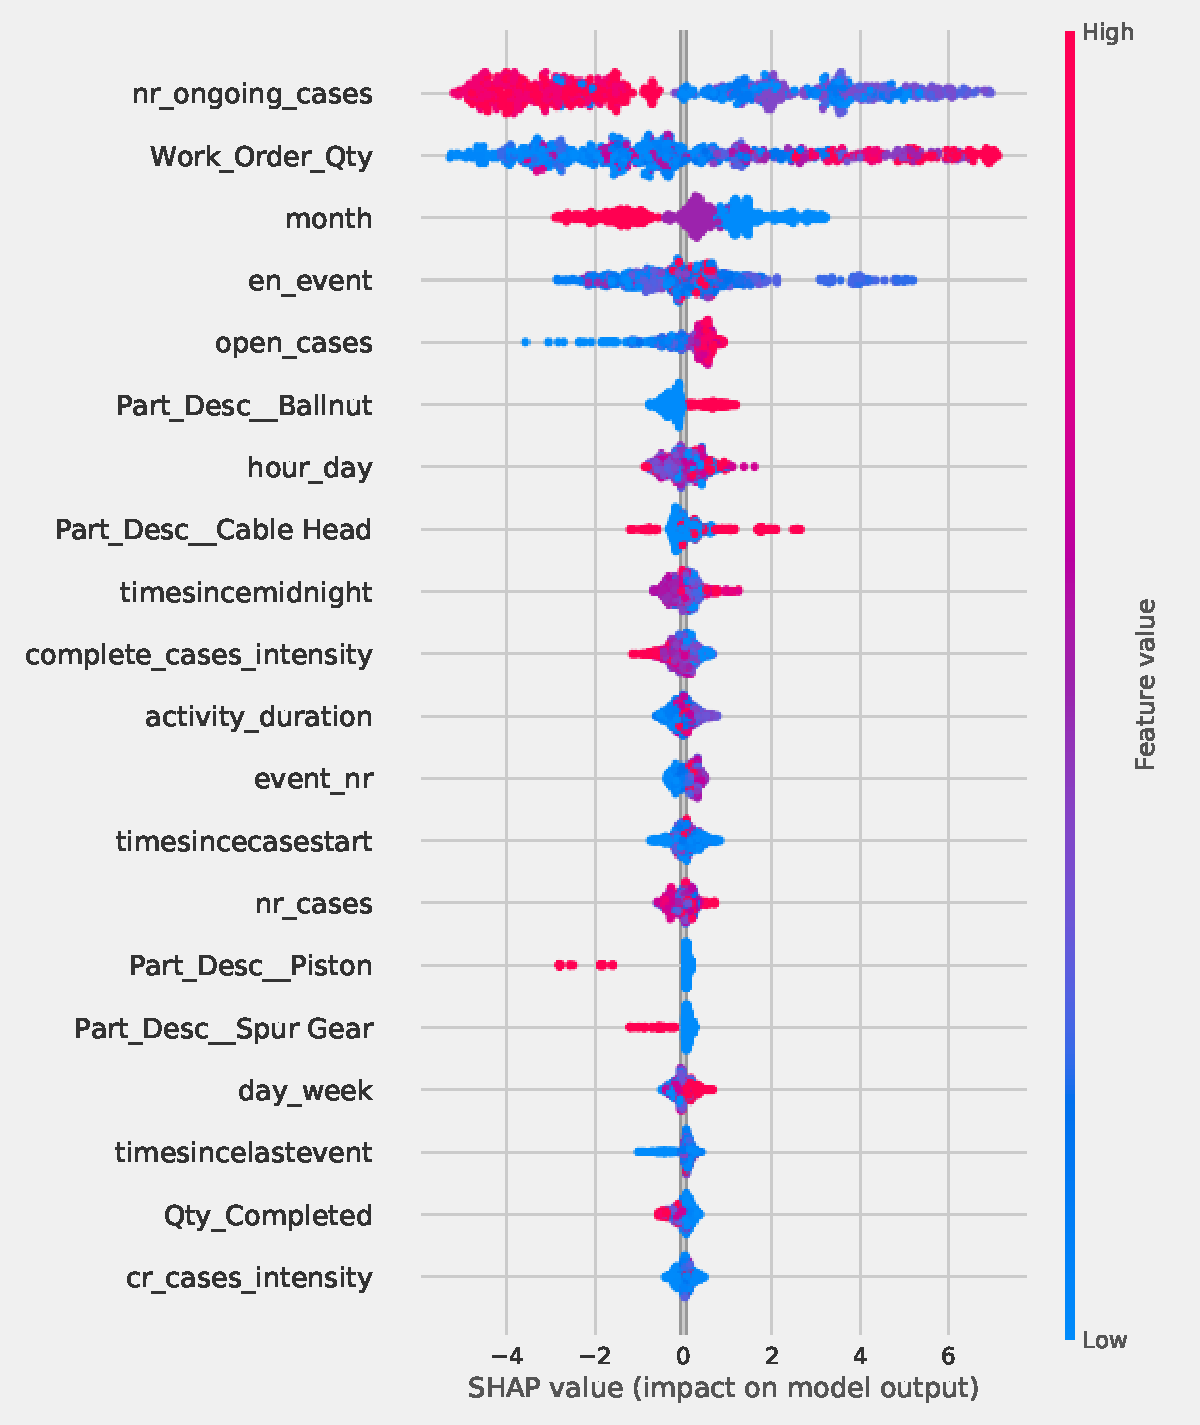
\includegraphics[width=\linewidth]{images/shap/summary_plot.pdf}
		\caption[SHAP density plot]{SHAP density plot of SHAP values for every feature to recognize how serious impact every feature holds on the model output}
	 \label{fig:SHAP11}
	\end{subfigure}\hspace*{\fill}
	\begin{subfigure}{0.48\textwidth}
		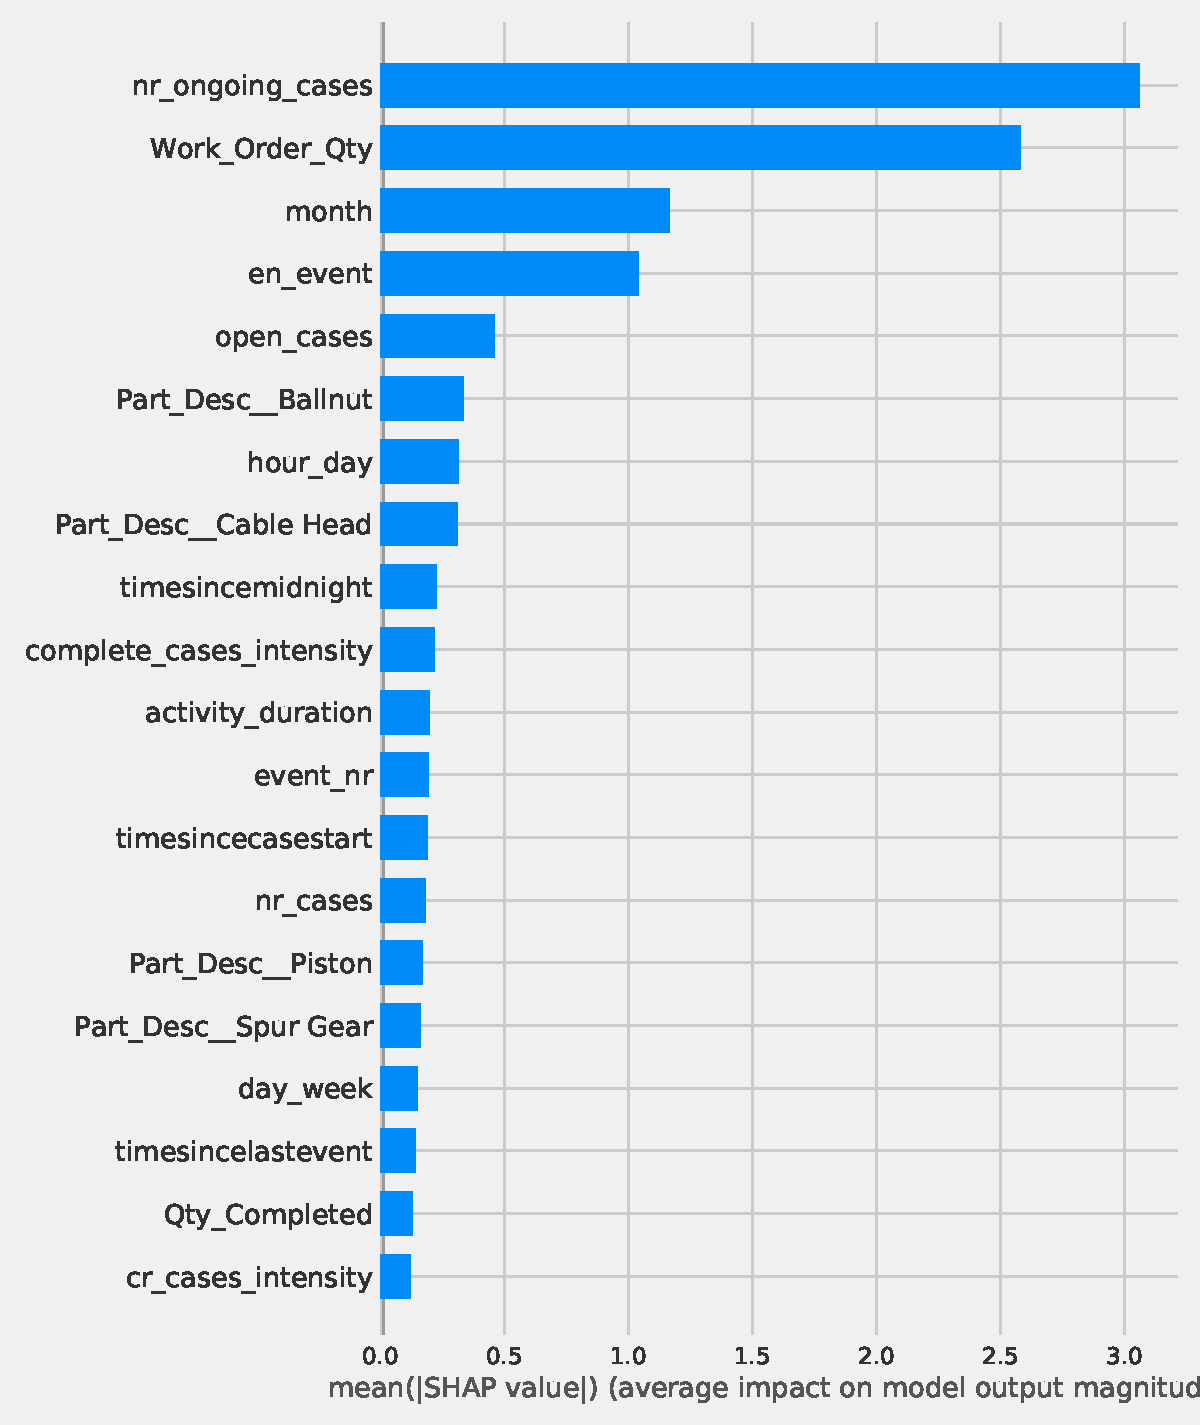
\includegraphics[width=\linewidth]{images/shap/feature_importance.pdf}
		\caption[SHAP feature importance plot]{SHAP feature importance plot based on the average of the SHAP value measures over the event log }
		\label{fig:shap12}
	\end{subfigure}\hspace*{\fill}
\end{figure}


Finally, we can see in figure \ref{fig:shappdp}, a SHAP dependence plot that shows the impact of a one (or pair) feature over the entire event log. Partial dependence plot (PDP) shows a relation between feature values and SHAP values which is corresponding to this same feature over different cases. Exactly the same as we saw before a higher number of ongoing cases have a significant impact on the positive outcome of the model, and vice versa for a negative outcome. 

\begin{figure}[!htbp]
	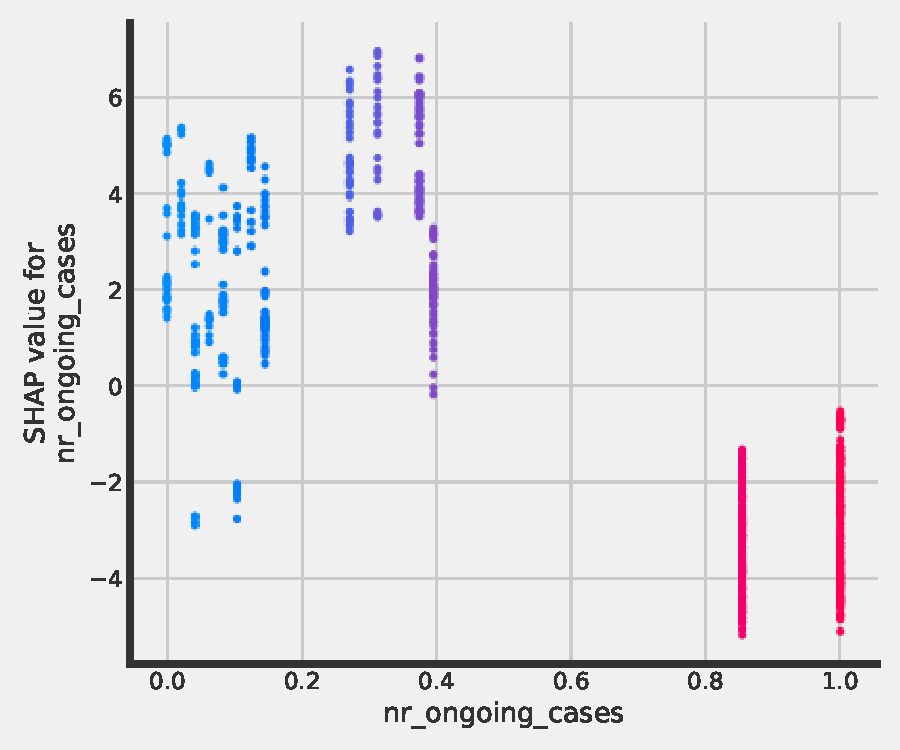
\includegraphics[width=\linewidth]{images/shap/pdp_nr_ongoing.pdf}
	\caption[SHAP dependence plots]{SHAP dependence plots}
	\label{fig:shappdp}
\end{figure}\hspace*{\fill}

After interpreting our outcome-oriented models based on the proposed inter-case features using SHAP analysis, we conclude that four out of nine proposed inter-case features have a significant impact on the model outcome. Accordingly, the jump in performance values for different classification models happen due to the huge effect of our inter-case features in particular \textit{nr\_ongoing\_cases} feature. 

%\clearpage
\section{Results: time performance}
In this section, we report the time measurements which is corresponding to the efficiency metric (see section \ref{evm}) for all methods that we proposed in this thesis. 




\subsection{CatBoost results:} \label{cr}
Predictive models are assumed to take much time during the training process while in the prediction time, it is better to be near real-time. In offline (or training) phase using CatBoost with larger event log such as \textit{BPIC2017, or Traffic fine} (see figure \ref{fig:T1}) on average is faster than XGBoost. On the other hand, using it with smaller event logs such as \textit{Production} it's more or less the same as XGBoost (see figure \ref{fig:T2}). \textit{Sparse} data is a bottleneck to  CatBoost during the training step, and it becomes slower than XGBoost and other methods.  In online (or prediction) time we can say that CatBoost is on average the fastest method (see figure \ref{fig:pT2}) in most of the event logs and it does not matter if the original event log is bigger or not because we are dealing with a stream of incoming events.



\begin{figure}[!htbp] % "[t!]" placement specifier just for this example
	
	\begin{subfigure}{0.48\textwidth}
		\includegraphics[width=\linewidth]{images/catboost/time/catboost/offline/bpic2017_A.pdf}
		
		%bpic2017_A.pdf}
		\caption{Execution time bpic2017\_A} \label{fig:t1}
	\end{subfigure}\hspace*{\fill}
	\begin{subfigure}{0.48\textwidth}
		\includegraphics[width=\linewidth]{images/catboost/time/catboost/offline/traffic.pdf}
		
		%traffic.pdf}
		\caption{Execution time Traffic} \label{fig:t2}
	\end{subfigure}\hspace*{\fill}
	\caption[Execution time comparison (offline)]{Execution time for models on large event logs such as BPIC2017, and Traffic fine logs. (training time)}
\label{fig:T1}
\end{figure}

\begin{figure}[!htbp] % "[t!]" placement specifier just for this example
	
	\begin{subfigure}{0.48\textwidth}
		\includegraphics[width=\linewidth]{images/catboost/time/catboost/offline/production.pdf}
		%			production.pdf}
		\caption{Execution time Production} \label{fig:t3}
	\end{subfigure}\hspace*{\fill}
	\begin{subfigure}{0.48\textwidth}
		\includegraphics[width=\linewidth]{images/catboost/time/catboost/offline/sepsis_1.pdf}
		
		%sepsis_1.pdf}
		\caption{Execution time Sepsis\_1} \label{fig:t4}
	\end{subfigure}\hspace*{\fill}
\caption[Execution time comparison (offline)]{Execution time for models on small event logs such as Production, and  Sepsis cases logs. (training time)}
%\caption{Time comparison between all methods with small event logs (Offline)}
\label{fig:T2}
\end{figure}

\begin{figure}[!htbp] % "[t!]" placement specifier just for this example

	\begin{subfigure}{0.48\textwidth}
		\includegraphics[width=\linewidth]{images/catboost/time/catboost/online/bpic2017_R.pdf}
		
		%pbpic2017_R.pdf}
		\caption{Execution time BPIC2017\_R (online)} \label{fig:t3}
	\end{subfigure}\hspace*{\fill}
	\begin{subfigure}{0.48\textwidth}
		\includegraphics[width=\linewidth]{images/catboost/time/catboost/online/sepsis_2.pdf}
		
		%psepsis_2.pdf}
		\caption{Execution time Sepsis\_2 (online)} \label{fig:t4}
	\end{subfigure}\hspace*{\fill}
	\caption[Execution time comparison (online)]{Execution time for models on large and small event logs such as BPIC2017, and Sepsis logs. (prediction time)}
%\caption{Execution time in (Online) phase}
\label{fig:pT2}
\end{figure}

%%%%%%%%%%%%%%%% TIME CATBOOST

\begin{table}[!htbp]
	\caption{Execution times for \textbf{CatBoost}}
	\label{tab:tc1}
	\centering
	\resizebox{0.75\textwidth}{!}{%
		\begin{tabular}{llllllll}
			
			
			\toprule
			& \multicolumn{2}{c}{{\bfseries bpic2015\_2}} & \multicolumn{2}{c}{{\bfseries bpic2012\_C}} & \multicolumn{2}{c}{{\bfseries bpic2015\_4}} \\ \cmidrule(lr){2-3} \cmidrule(lr){4-5} \cmidrule(lr){6-7}
			method  & training\_total (s) & prediction\_avg (ms) & training\_total (s) & prediction\_avg (ms) & training\_total (s) & prediction\_avg (ms) \\ \midrule
			cluster\_laststate & $4035.1 \pm 27.6$ & $77.51 \pm 0.05$ & $5392.83 \pm 42.3$ & $55.1 \pm 0.03$ & $\mathbf{67.48 \pm 43.54}$ & $115.84 \pm 0.06$ \\ 
			cluster\_agg & $425067.1 \pm 24.19$ & $24.84 \pm 0.03$ & $112428.33 \pm 26.27$ & $29.36 \pm 0.03$ & $20969.05 \pm 25.85$ & $26.38 \pm 0.03$ \\ 
			single\_agg & $407.26 \pm 45.59$ & $82.14 \pm 0.03$ & $297.85 \pm 41.59$ & $28.26 \pm 0.01$ & $75.38 \pm 26.51$ & $156.81 \pm 0.06$ \\ 
			prefix\_agg & $8788.2 \pm 22.76$ & $38.55 \pm 40.05$ & $8829.17 \pm 31.6$ & $37.0 \pm 30.16$ & $8260.38 \pm 30.58$ & $36.17 \pm 22.18$ \\ 
			prefix\_laststate & $1575.81 \pm 24.55$ & $28.33 \pm 44.55$ & $2087.29 \pm 35.0$ & $39.28 \pm 34.76$ & $1084.4 \pm 41.17$ & $60.54 \pm 37.11$ \\ 
			single\_laststate & $\mathbf{255.6 \pm 28.38}$ & $60.07 \pm 0.02$ & $525.63 \pm 45.56$ & $\mathbf{27.49 \pm 0.01}$ & $111.92 \pm 41.15$ & $44.08 \pm 0.01$ \\ 
			prefix\_index & $366.63 \pm 23.15$ & $23.34 \pm 34.86$ & $874.61 \pm 26.28$ & $30.16 \pm 31.67$ & $208.21 \pm 25.37$ & $44.1 \pm 32.57$ \\ 
			state\_agg & $276.57 \pm 44.63$ & $\mathbf{18.43 \pm 0.01}$ & $3130.88 \pm 30.61$ & $42.69 \pm 0.01$ & $1742.07 \pm 32.16$ & $26.05 \pm 0.01$ \\ 
			state\_laststate & $337.11 \pm 40.79$ & $31.68 \pm 0.01$ & $\mathbf{20.36 \pm 40.39}$ & $32.51 \pm 0.01$ & $257.69 \pm 21.02$ & $\mathbf{20.94 \pm 0.0}$ \\ 
			\bottomrule
			\toprule
			& \multicolumn{2}{c}{{\bfseries bpic2012\_D}} & \multicolumn{2}{c}{{\bfseries bpic2017\_A}} & \multicolumn{2}{c}{{\bfseries bpic2011\_4}} \\ \cmidrule(lr){2-3} \cmidrule(lr){4-5} \cmidrule(lr){6-7}
			method  & training\_total (s) & prediction\_avg (ms) & training\_total (s) & prediction\_avg (ms) & training\_total (s) & prediction\_avg (ms) \\ \midrule
			cluster\_laststate & $815.78 \pm 35.58$ & $48.4 \pm 0.02$ & $732.62 \pm 32.4$ & $65.62 \pm 0.02$ & $340.59 \pm 26.76$ & $103.05 \pm 0.05$ \\ 
			cluster\_agg & $214560.64 \pm 23.54$ & $\mathbf{26.48 \pm 0.03}$ & $262684.18 \pm 24.33$ & $34.85 \pm 0.03$ & $136208.45 \pm 38.74$ & $61.2 \pm 0.06$ \\ 
			single\_agg & $1456.56 \pm 40.4$ & $28.45 \pm 0.01$ & $2985.75 \pm 21.3$ & $43.63 \pm 0.01$ & $\mathbf{84.08 \pm 31.63}$ & $44.92 \pm 0.02$ \\ 
			prefix\_agg & $8531.68 \pm 24.16$ & $32.01 \pm 31.66$ & $21626.27 \pm 43.03$ & $\mathbf{18.77 \pm 23.1}$ & $3733.45 \pm 22.92$ & $28.76 \pm 34.18$ \\ 
			prefix\_laststate & $1623.02 \pm 38.17$ & $37.97 \pm 36.06$ & $3918.62 \pm 24.78$ & $29.37 \pm 32.87$ & $679.86 \pm 38.96$ & $54.3 \pm 48.75$ \\ 
			single\_laststate & $\mathbf{688.33 \pm 47.94}$ & $27.68 \pm 0.01$ & $1424.59 \pm 32.63$ & $26.28 \pm 0.01$ & $147.98 \pm 42.73$ & $\mathbf{16.53 \pm 0.0}$ \\ 
			prefix\_index & $1157.14 \pm 31.24$ & $40.83 \pm 39.4$ & $4424.61 \pm 32.41$ & $24.95 \pm 44.41$ & $122.02 \pm 38.28$ & $23.27 \pm 43.07$ \\ 
			state\_agg & $4053.21 \pm 22.2$ & $42.79 \pm 0.01$ & $\mathbf{178.05 \pm 29.37}$ & $69.55 \pm 0.02$ & $317.15 \pm 46.9$ & $59.55 \pm 0.02$ \\ 
			state\_laststate & $18068.63 \pm 33.76$ & $33.61 \pm 0.01$ & $5698.17 \pm 28.83$ & $41.78 \pm 0.01$ & $280.86 \pm 42.4$ & $98.96 \pm 0.03$ \\ 
			\bottomrule
			\toprule
			& \multicolumn{2}{c}{{\bfseries traffic}} & \multicolumn{2}{c}{{\bfseries bpic2012\_A}} & \multicolumn{2}{c}{{\bfseries bpic2015\_3}} \\ \cmidrule(lr){2-3} \cmidrule(lr){4-5} \cmidrule(lr){6-7}
			method  & training\_total (s) & prediction\_avg (ms) & training\_total (s) & prediction\_avg (ms) & training\_total (s) & prediction\_avg (ms) \\ \midrule
			cluster\_laststate & $617.97 \pm 39.02$ & $191.29 \pm 0.03$ & $5726.52 \pm 28.41$ & $53.35 \pm 0.03$ & $\mathbf{141.09 \pm 23.81}$ & $89.93 \pm 0.05$ \\ 
			cluster\_agg & $136871.63 \pm 24.19$ & $105.33 \pm 0.04$ & $292502.98 \pm 45.11$ & $25.63 \pm 0.03$ & $146380.45 \pm 49.55$ & $27.19 \pm 0.03$ \\ 
			single\_agg & $545.66 \pm 39.0$ & $132.31 \pm 0.02$ & $\mathbf{167.15 \pm 45.24}$ & $\mathbf{22.56 \pm 0.01}$ & $251.5 \pm 49.6$ & $178.36 \pm 0.07$ \\ 
			prefix\_agg & $18164.8 \pm 36.76$ & $36.3 \pm 25.2$ & $7348.92 \pm 45.24$ & $34.7 \pm 38.34$ & $17847.98 \pm 42.98$ & $34.85 \pm 32.02$ \\ 
			prefix\_laststate & $3421.21 \pm 44.07$ & $55.12 \pm 38.89$ & $1604.91 \pm 40.15$ & $63.84 \pm 32.87$ & $2360.49 \pm 25.56$ & $57.44 \pm 44.94$ \\ 
			single\_laststate & $1508.39 \pm 49.12$ & $85.48 \pm 0.01$ & $502.66 \pm 49.0$ & $27.52 \pm 0.01$ & $307.66 \pm 27.58$ & $43.78 \pm 0.01$ \\ 
			prefix\_index & $16493.67 \pm 45.46$ & $\mathbf{24.27 \pm 33.08}$ & $1162.18 \pm 48.76$ & $24.65 \pm 29.64$ & $519.29 \pm 31.66$ & $41.86 \pm 44.17$ \\ 
			state\_agg & $\mathbf{355.86 \pm 43.55}$ & $228.84 \pm 0.03$ & $752.18 \pm 21.48$ & $75.63 \pm 0.02$ & $5062.38 \pm 31.58$ & $\mathbf{19.79 \pm 0.01}$ \\ 
			state\_laststate & $4411.24 \pm 23.22$ & $126.22 \pm 0.02$ & $1227.07 \pm 44.28$ & $45.05 \pm 0.01$ & $348.02 \pm 42.56$ & $29.17 \pm 0.01$ \\ 
			\bottomrule
			\toprule
			& \multicolumn{2}{c}{{\bfseries bpic2011\_3}} & \multicolumn{2}{c}{{\bfseries bpic2011\_2}} & \multicolumn{2}{c}{{\bfseries sepsis\_2}} \\ \cmidrule(lr){2-3} \cmidrule(lr){4-5} \cmidrule(lr){6-7}
			method  & training\_total (s) & prediction\_avg (ms) & training\_total (s) & prediction\_avg (ms) & training\_total (s) & prediction\_avg (ms) \\ \midrule
			cluster\_laststate & $\mathbf{89.67 \pm 48.8}$ & $113.89 \pm 0.05$ & $\mathbf{49.63 \pm 22.59}$ & $105.55 \pm 0.05$ & $95.29 \pm 32.56$ & $80.4 \pm 0.03$ \\ 
			cluster\_agg & $86472.7 \pm 44.97$ & $107.02 \pm 0.1$ & $61273.31 \pm 32.75$ & $95.88 \pm 0.11$ & $2862494.55 \pm 41.88$ & $78.42 \pm 0.06$ \\ 
			single\_agg & $154.05 \pm 28.92$ & $58.65 \pm 0.02$ & $103.01 \pm 34.63$ & $49.87 \pm 0.02$ & $\mathbf{50.57 \pm 46.54}$ & $83.61 \pm 0.02$ \\ 
			prefix\_agg & $1640.77 \pm 45.98$ & $38.4 \pm 38.76$ & $3522.71 \pm 45.65$ & $21.45 \pm 35.65$ & $475.74 \pm 40.06$ & $\mathbf{22.46 \pm 37.92}$ \\ 
			prefix\_laststate & $327.68 \pm 25.27$ & $39.2 \pm 48.2$ & $762.27 \pm 47.93$ & $31.09 \pm 34.11$ & $90.68 \pm 23.82$ & $33.84 \pm 21.77$ \\ 
			single\_laststate & $101.73 \pm 39.45$ & $\mathbf{20.95 \pm 0.01}$ & $202.65 \pm 33.1$ & $\mathbf{15.78 \pm 0.0}$ & $2061.4 \pm 23.47$ & $69.08 \pm 0.01$ \\ 
			prefix\_index & $114.68 \pm 28.55$ & $48.19 \pm 45.26$ & $127.64 \pm 28.45$ & $41.89 \pm 31.75$ & $103.84 \pm 40.16$ & $34.69 \pm 26.72$ \\ 
			state\_agg & $422.62 \pm 29.68$ & $82.29 \pm 0.02$ & $523.02 \pm 33.51$ & $59.7 \pm 0.02$ & $3822.72 \pm 25.15$ & $82.25 \pm 0.02$ \\ 
			state\_laststate & $343.87 \pm 43.47$ & $98.45 \pm 0.02$ & $193.67 \pm 27.01$ & $90.83 \pm 0.03$ & $91.67 \pm 29.95$ & $182.92 \pm 0.03$ \\ 
			\bottomrule
			\toprule
			& \multicolumn{2}{c}{{\bfseries bpic2015\_1}} & \multicolumn{2}{c}{{\bfseries bpic2015\_5}} & \multicolumn{2}{c}{{\bfseries sepsis\_3}} \\ \cmidrule(lr){2-3} \cmidrule(lr){4-5} \cmidrule(lr){6-7}
			method  & training\_total (s) & prediction\_avg (ms) & training\_total (s) & prediction\_avg (ms) & training\_total (s) & prediction\_avg (ms) \\ \midrule
			cluster\_laststate & $92.35 \pm 47.68$ & $49.43 \pm 0.02$ & $165.75 \pm 21.57$ & $110.39 \pm 0.06$ & $2046.66 \pm 37.68$ & $64.78 \pm 0.02$ \\ 
			cluster\_agg & $2614134.85 \pm 45.94$ & $30.22 \pm 0.03$ & $19001.6 \pm 39.57$ & $33.35 \pm 0.04$ & $16298503.69 \pm 45.75$ & $57.33 \pm 0.05$ \\ 
			single\_agg & $185.25 \pm 35.31$ & $77.48 \pm 0.03$ & $122.79 \pm 30.3$ & $212.25 \pm 0.08$ & $1255.99 \pm 25.72$ & $72.8 \pm 0.02$ \\ 
			prefix\_agg & $7671.38 \pm 31.1$ & $34.54 \pm 42.26$ & $11688.96 \pm 34.73$ & $35.25 \pm 35.74$ & $1402.76 \pm 43.85$ & $\mathbf{31.66 \pm 27.51}$ \\ 
			prefix\_laststate & $1358.18 \pm 44.4$ & $45.65 \pm 20.76$ & $2022.84 \pm 34.34$ & $32.79 \pm 48.92$ & $270.83 \pm 22.22$ & $48.13 \pm 34.91$ \\ 
			single\_laststate & $80.92 \pm 45.55$ & $65.91 \pm 0.02$ & $610.51 \pm 20.8$ & $59.06 \pm 0.02$ & $126.26 \pm 35.17$ & $57.55 \pm 0.01$ \\ 
			prefix\_index & $256.4 \pm 21.77$ & $48.89 \pm 34.32$ & $521.86 \pm 38.13$ & $43.87 \pm 32.48$ & $105.52 \pm 31.67$ & $38.86 \pm 29.15$ \\ 
			state\_agg & $\mathbf{64.95 \pm 35.87}$ & $19.7 \pm 0.01$ & $147.38 \pm 42.92$ & $24.11 \pm 0.01$ & $4657.35 \pm 27.14$ & $66.51 \pm 0.02$ \\ 
			state\_laststate & $120.37 \pm 49.72$ & $\mathbf{16.41 \pm 0.0}$ & $\mathbf{100.01 \pm 44.41}$ & $\mathbf{14.73 \pm 0.0}$ & $\mathbf{32.92 \pm 38.47}$ & $143.57 \pm 0.03$ \\ 
			\bottomrule
			\toprule
			& \multicolumn{2}{c}{{\bfseries bpic2017\_C}} & \multicolumn{2}{c}{{\bfseries production}} & \multicolumn{2}{c}{{\bfseries sepsis\_1}} \\ \cmidrule(lr){2-3} \cmidrule(lr){4-5} \cmidrule(lr){6-7}
			method  & training\_total (s) & prediction\_avg (ms) & training\_total (s) & prediction\_avg (ms) & training\_total (s) & prediction\_avg (ms) \\ \midrule
			cluster\_laststate & $10772.93 \pm 33.26$ & $68.79 \pm 0.03$ & $139.26 \pm 44.45$ & $64.07 \pm 0.02$ & $24.53 \pm 39.11$ & $61.16 \pm 0.02$ \\ 
			cluster\_agg & $114443.62 \pm 28.67$ & $36.6 \pm 0.03$ & $31414.7 \pm 43.16$ & $43.86 \pm 0.03$ & $80600.81 \pm 33.14$ & $70.65 \pm 0.06$ \\ 
			
			single\_agg & $2270.8 \pm 35.67$ & $40.6 \pm 0.01$ & $110.04 \pm 38.96$ & $127.63 \pm 0.03$ & $96.49 \pm 44.2$ & $73.18 \pm 0.02$ \\ 
			prefix\_agg & $20727.33 \pm 36.81$ & $40.96 \pm 46.28$ & $530.54 \pm 36.03$ & $\mathbf{20.01 \pm 39.1}$ & $1348.64 \pm 46.77$ & $\mathbf{26.36 \pm 28.4}$ \\ 
			prefix\_laststate & $2816.38 \pm 31.59$ & $32.16 \pm 39.09$ & $103.66 \pm 45.82$ & $28.38 \pm 47.32$ & $271.41 \pm 45.06$ & $40.03 \pm 47.92$ \\ 
			single\_laststate & $541.76 \pm 25.16$ & $29.1 \pm 0.01$ & $96.73 \pm 36.41$ & $32.89 \pm 0.0$ & $320.38 \pm 32.87$ & $62.25 \pm 0.01$ \\ 
			prefix\_index & $4205.79 \pm 27.01$ & $\mathbf{22.88 \pm 49.9}$ & $24.45 \pm 26.57$ & $32.09 \pm 41.17$ & $99.68 \pm 28.32$ & $26.85 \pm 35.73$ \\ 
			state\_agg & $756.35 \pm 34.38$ & $59.65 \pm 0.02$ & $110.15 \pm 21.7$ & $101.65 \pm 0.02$ & $\mathbf{10.5 \pm 21.92}$ & $46.98 \pm 0.01$ \\ 
			state\_laststate & $\mathbf{246.39 \pm 33.0}$ & $74.08 \pm 0.02$ & $\mathbf{13.4 \pm 44.45}$ & $48.59 \pm 0.01$ & $351.73 \pm 23.16$ & $127.0 \pm 0.02$ \\ 
			\bottomrule
			\toprule
			& \multicolumn{2}{c}{{\bfseries bpic2011\_1}} & \multicolumn{2}{c}{{\bfseries bpic2017\_R}} \\ \cmidrule(lr){2-3} \cmidrule(lr){4-5} \cmidrule(lr){6-7}
			method  & training\_total (s) & prediction\_avg (ms) & training\_total (s) & prediction\_avg (ms) \\ \midrule
			cluster\_laststate & $848.63 \pm 20.93$ & $104.77 \pm 0.05$ & $837.23 \pm 21.12$ & $52.23 \pm 0.02$ \\ 
			cluster\_agg & $65724.68 \pm 47.54$ & $65.95 \pm 0.05$ & $7436286.17 \pm 24.4$ & $27.04 \pm 0.02$ \\ 
			single\_agg & $\mathbf{34.98 \pm 42.04}$ & $57.16 \pm 0.03$ & $8619.04 \pm 44.48$ & $40.29 \pm 0.01$ \\ 
			prefix\_agg & $2262.18 \pm 42.89$ & $25.48 \pm 36.77$ & $23969.9 \pm 25.89$ & $\mathbf{22.68 \pm 21.44}$ \\ 
			prefix\_laststate & $485.91 \pm 21.47$ & $46.61 \pm 30.32$ & $4084.31 \pm 40.61$ & $42.28 \pm 40.28$ \\ 
			single\_laststate & $68.88 \pm 32.63$ & $\mathbf{18.22 \pm 0.0}$ & $5017.23 \pm 39.54$ & $28.33 \pm 0.01$ \\ 
			prefix\_index & $115.67 \pm 40.37$ & $49.92 \pm 24.23$ & $4604.51 \pm 24.8$ & $28.19 \pm 43.45$ \\ 
			state\_agg & $1637.66 \pm 42.2$ & $74.57 \pm 0.02$ & $8506.42 \pm 28.53$ & $53.61 \pm 0.01$ \\ 
			state\_laststate & $469.56 \pm 44.77$ & $100.15 \pm 0.03$ & $\mathbf{344.58 \pm 28.21}$ & $39.75 \pm 0.01$ \\ 
			\bottomrule
			
		\end{tabular}%
	}
	
	
\end{table}



Execution times for all bucketing, encoding and classification methods are computed across five equal executions employing the best optimal parameters, are shown in Table \ref{tab:tc1} (CatBoost), Table  \ref{tab:cxgbt} (XGBoost), Table \ref{tab:clogitt} (Logit), Table \ref{tab:crft} (RF), and Table  \ref{tab:csvmt} (SVM).







%%%%%%%%%%%%%%%%%%%%


\subsection{Complex sequence encoding (Wavelet) results:}
Wavelet encoding method achieved improvement w.r.t the prediction accuracy in most of the event logs, however, for the execution time it takes much time just to encode each event log into a feature matrix as the time complexity for this method is $O(n^3)$. Table \ref{tab:twc1} shows the execution time of wavelet encoding and CatBoost classifier. Table \ref{tab:twx1} (XGBoost), Table \ref{tab:twr1} (RF), Table \ref{tab:twl1} (Logit), and Table \ref{tab:tws1} (SVM).


To show the difference between offline and online execution times, we compare this execution time with the previous encoding methods in contribution 1 section \ref{cr} results.  For example, figure \ref{fig:wT1} shows the difference between wavelet and other techniques w.r.t production event log during the training process, while figure \ref{fig:wT2} shows the same compression but for prediction (or online) phase. We can conclude that using the wavelet encoding method; our predictive model suffers from a huge amount of time to train and to predict any running business case, which could be a good direction in future work to improve the time complexity of this encoding method. 

\begin{figure}[!htbp] % "[t!]" placement specifier just for this example
	
	\begin{subfigure}{0.48\textwidth}
		\includegraphics[width=\linewidth]{images/wavelet/time/cat_production.pdf}
		\caption{Without wavelet} \label{fig:tw1}
	\end{subfigure}\hspace*{\fill}
	\begin{subfigure}{0.48\textwidth}
		\includegraphics[width=\linewidth]{images/wavelet/time/wavelet_production.pdf}
		\caption{With wavelet} \label{fig:tw2}
	\end{subfigure}\hspace*{\fill}
	\caption{Execution time before and after adding the wavelet encoding method (training) on Production event log}
\label{fig:wT1}
\end{figure}

\begin{figure}[!htbp] % "[t!]" placement specifier just for this example

	\begin{subfigure}{0.48\textwidth}
		\includegraphics[width=\linewidth]{images/wavelet/time/p_c_production.pdf}
		\caption{Without wavelet} \label{fig:tw3}
	\end{subfigure}\hspace*{\fill}
	\begin{subfigure}{0.48\textwidth}
		\includegraphics[width=\linewidth]{images/wavelet/time/p_w_production.pdf}
		\caption{With wavelet} \label{fig:tw2}
	\end{subfigure}\hspace*{\fill}
		\caption{Execution time before and after adding the wavelet encoding method (online) on Production event log}
	\label{fig:wT2}
\end{figure}





%%%%%%%%%%%%%%%% TIME CATBOOST

\begin{table}[!htbp]
	\caption{Execution times for \textbf{Wavelet plus CatBoost}}
	\label{tab:twc1}
	\centering
	\resizebox{0.8\textwidth}{!}{%
		\begin{tabular}{llllllll}
			\toprule
			& \multicolumn{2}{c}{{\bfseries bpic2015\_2}} & \multicolumn{2}{c}{{\bfseries bpic2012\_C}} & \multicolumn{2}{c}{{\bfseries bpic2015\_4}} \\ \cmidrule(lr){2-3} \cmidrule(lr){4-5} \cmidrule(lr){6-7}
			method  & training\_total (s) & prediction\_avg (ms) & training\_total (s) & prediction\_avg (ms) & training\_total (s) & prediction\_avg (ms) \\ \midrule
			cluster\_WaveletLast & $22879.0 \pm 156.51$ & $439.49 \pm 0.28$ & $30577.36 \pm 239.83$ & $312.39 \pm 0.16$ & $\mathbf{382.61 \pm 246.88}$ & $656.8 \pm 0.36$ \\ 
			prefix\_waveletLast & $8934.83 \pm 139.22$ & $160.65 \pm 252.58$ & $11834.96 \pm 198.46$ & $222.73 \pm 197.11$ & $6148.53 \pm 233.44$ & $343.24 \pm 210.43$ \\ 
			state\_waveletAgg & $1568.13 \pm 253.02$ & $\mathbf{104.51 \pm 0.03}$ & $17752.08 \pm 173.56$ & $242.03 \pm 0.07$ & $9877.56 \pm 182.33$ & $147.71 \pm 0.05$ \\ 
			single\_waveletLast & $\mathbf{1449.25 \pm 160.91}$ & $340.61 \pm 0.1$ & $2980.32 \pm 258.32$ & $\mathbf{155.86 \pm 0.04}$ & $634.6 \pm 233.32$ & $249.95 \pm 0.08$ \\ 
			single\_waveletAgg & $2309.17 \pm 258.5$ & $465.72 \pm 0.18$ & $1688.82 \pm 235.79$ & $160.24 \pm 0.06$ & $427.41 \pm 150.31$ & $889.14 \pm 0.33$ \\ 
			state\_waveletLast & $1911.44 \pm 231.25$ & $179.62 \pm 0.06$ & $\mathbf{115.45 \pm 229.03}$ & $184.33 \pm 0.04$ & $1461.12 \pm 119.17$ & $\mathbf{118.75 \pm 0.03}$ \\ 
			prefix\_waveletAgg & $49829.08 \pm 129.06$ & $218.57 \pm 227.11$ & $50061.39 \pm 179.17$ & $209.77 \pm 170.98$ & $46836.34 \pm 173.41$ & $205.06 \pm 125.74$ \\ 
			cluster\_WaveletAgg & $2410130.43 \pm 137.17$ & $140.82 \pm 0.15$ & $637468.64 \pm 148.93$ & $166.49 \pm 0.18$ & $118894.5 \pm 146.59$ & $149.58 \pm 0.15$ \\ 
			prefix\_waveletIndex & $2078.79 \pm 131.29$ & $132.36 \pm 197.68$ & $4959.04 \pm 149.02$ & $170.99 \pm 179.56$ & $1180.58 \pm 143.87$ & $250.05 \pm 184.69$ \\ 
			\bottomrule
			\toprule
			& \multicolumn{2}{c}{{\bfseries bpic2012\_D}} & \multicolumn{2}{c}{{\bfseries bpic2017\_A}} & \multicolumn{2}{c}{{\bfseries bpic2011\_4}} \\ \cmidrule(lr){2-3} \cmidrule(lr){4-5} \cmidrule(lr){6-7}
			method  & training\_total (s) & prediction\_avg (ms) & training\_total (s) & prediction\_avg (ms) & training\_total (s) & prediction\_avg (ms) \\ \midrule
			cluster\_WaveletLast & $4625.45 \pm 201.71$ & $274.44 \pm 0.13$ & $4153.96 \pm 183.72$ & $372.06 \pm 0.14$ & $1931.14 \pm 151.72$ & $584.32 \pm 0.3$ \\ 
			prefix\_waveletLast & $9202.54 \pm 216.43$ & $215.31 \pm 204.45$ & $22218.56 \pm 140.5$ & $166.51 \pm 186.38$ & $3854.81 \pm 220.92$ & $307.87 \pm 276.41$ \\ 
			state\_waveletAgg & $22981.67 \pm 125.89$ & $242.6 \pm 0.08$ & $\mathbf{1009.56 \pm 166.52}$ & $394.38 \pm 0.09$ & $1798.21 \pm 265.92$ & $337.64 \pm 0.1$ \\ 
			single\_waveletLast & $\mathbf{3902.82 \pm 271.8}$ & $156.92 \pm 0.04$ & $8077.42 \pm 184.99$ & $149.0 \pm 0.03$ & $839.07 \pm 242.28$ & $\mathbf{93.72 \pm 0.03}$ \\ 
			single\_waveletAgg & $8258.69 \pm 229.09$ & $161.29 \pm 0.07$ & $16929.19 \pm 120.77$ & $247.36 \pm 0.07$ & $\mathbf{476.71 \pm 179.34}$ & $254.71 \pm 0.11$ \\ 
			state\_waveletLast & $102449.13 \pm 191.44$ & $190.57 \pm 0.06$ & $32308.61 \pm 163.49$ & $236.88 \pm 0.05$ & $1592.47 \pm 240.39$ & $561.09 \pm 0.15$ \\ 
			prefix\_waveletAgg & $48374.64 \pm 137.01$ & $181.48 \pm 179.54$ & $122620.94 \pm 243.97$ & $\mathbf{106.42 \pm 131.0}$ & $21168.69 \pm 129.97$ & $163.08 \pm 193.8$ \\ 
			cluster\_WaveletAgg & $1216558.85 \pm 133.45$ & $\mathbf{150.15 \pm 0.15}$ & $1489419.31 \pm 137.93$ & $197.6 \pm 0.16$ & $772301.89 \pm 219.67$ & $347.0 \pm 0.32$ \\ 
			prefix\_waveletIndex & $6560.96 \pm 177.14$ & $231.5 \pm 223.4$ & $25087.55 \pm 183.79$ & $141.49 \pm 251.78$ & $691.86 \pm 217.05$ & $131.92 \pm 244.23$ \\ 
			\bottomrule
			\toprule
			& \multicolumn{2}{c}{{\bfseries traffic}} & \multicolumn{2}{c}{{\bfseries bpic2012\_A}} & \multicolumn{2}{c}{{\bfseries bpic2015\_3}} \\ \cmidrule(lr){2-3} \cmidrule(lr){4-5} \cmidrule(lr){6-7}
			method  & training\_total (s) & prediction\_avg (ms) & training\_total (s) & prediction\_avg (ms) & training\_total (s) & prediction\_avg (ms) \\ \midrule
			cluster\_WaveletLast & $3503.88 \pm 221.25$ & $1084.64 \pm 0.18$ & $32469.38 \pm 161.08$ & $302.52 \pm 0.15$ & $\mathbf{799.96 \pm 134.97}$ & $509.89 \pm 0.27$ \\ 
			prefix\_waveletLast & $19398.28 \pm 249.89$ & $312.52 \pm 220.48$ & $9099.81 \pm 227.66$ & $361.97 \pm 186.37$ & $13383.99 \pm 144.93$ & $325.68 \pm 254.79$ \\ 
			state\_waveletAgg & $\mathbf{2017.72 \pm 246.95}$ & $1297.52 \pm 0.14$ & $4264.84 \pm 121.79$ & $428.82 \pm 0.14$ & $28703.68 \pm 179.04$ & $\mathbf{112.22 \pm 0.03}$ \\ 
			single\_waveletLast & $8552.55 \pm 278.53$ & $484.7 \pm 0.05$ & $2850.08 \pm 277.83$ & $156.02 \pm 0.04$ & $1744.44 \pm 156.36$ & $248.21 \pm 0.08$ \\ 
			single\_waveletAgg & $3093.89 \pm 221.15$ & $750.19 \pm 0.1$ & $\mathbf{947.75 \pm 256.5}$ & $\mathbf{127.93 \pm 0.05}$ & $1425.98 \pm 281.21$ & $1011.33 \pm 0.39$ \\ 
			state\_waveletLast & $25011.73 \pm 131.64$ & $715.64 \pm 0.09$ & $6957.5 \pm 251.05$ & $255.41 \pm 0.07$ & $1973.28 \pm 241.29$ & $165.37 \pm 0.05$ \\ 
			prefix\_waveletAgg & $102994.44 \pm 208.44$ & $205.82 \pm 142.91$ & $41668.39 \pm 256.53$ & $196.72 \pm 217.41$ & $101198.07 \pm 243.7$ & $197.61 \pm 181.53$ \\ 
			cluster\_WaveletAgg & $776062.15 \pm 137.14$ & $597.23 \pm 0.22$ & $1658491.89 \pm 255.75$ & $145.35 \pm 0.15$ & $829977.17 \pm 280.96$ & $154.18 \pm 0.15$ \\ 
			prefix\_waveletIndex & $93519.12 \pm 257.73$ & $\mathbf{137.62 \pm 187.55}$ & $6589.57 \pm 276.5$ & $139.76 \pm 168.08$ & $2944.38 \pm 179.5$ & $237.32 \pm 250.45$ \\ 
			\bottomrule
			\toprule
			& \multicolumn{2}{c}{{\bfseries bpic2011\_3}} & \multicolumn{2}{c}{{\bfseries bpic2011\_2}} & \multicolumn{2}{c}{{\bfseries sepsis\_2}} \\ \cmidrule(lr){2-3} \cmidrule(lr){4-5} \cmidrule(lr){6-7}
			method  & training\_total (s) & prediction\_avg (ms) & training\_total (s) & prediction\_avg (ms) & training\_total (s) & prediction\_avg (ms) \\ \midrule
			cluster\_WaveletLast & $\mathbf{508.42 \pm 276.7}$ & $645.74 \pm 0.31$ & $\mathbf{281.39 \pm 128.11}$ & $598.44 \pm 0.31$ & $540.32 \pm 184.63$ & $455.86 \pm 0.15$ \\ 
			prefix\_waveletLast & $1857.93 \pm 143.26$ & $222.26 \pm 273.29$ & $4322.05 \pm 271.76$ & $176.27 \pm 193.39$ & $514.16 \pm 135.06$ & $191.86 \pm 123.44$ \\ 
			state\_waveletAgg & $2396.27 \pm 168.3$ & $466.6 \pm 0.13$ & $2965.53 \pm 189.97$ & $338.51 \pm 0.11$ & $21674.84 \pm 142.6$ & $466.33 \pm 0.09$ \\ 
			single\_waveletLast & $576.83 \pm 223.69$ & $\mathbf{118.76 \pm 0.03}$ & $1149.02 \pm 187.66$ & $\mathbf{89.48 \pm 0.03}$ & $11688.12 \pm 133.08$ & $391.66 \pm 0.08$ \\ 
			single\_waveletAgg & $873.49 \pm 163.98$ & $332.55 \pm 0.13$ & $584.06 \pm 196.36$ & $282.79 \pm 0.13$ & $\mathbf{286.76 \pm 263.86}$ & $474.07 \pm 0.13$ \\ 
			state\_waveletLast & $1949.75 \pm 246.48$ & $558.22 \pm 0.14$ & $1098.09 \pm 153.14$ & $514.98 \pm 0.15$ & $519.78 \pm 169.83$ & $1037.17 \pm 0.19$ \\ 
			prefix\_waveletAgg & $9303.17 \pm 260.73$ & $217.71 \pm 219.76$ & $19973.74 \pm 258.86$ & $121.63 \pm 202.12$ & $2697.47 \pm 227.16$ & $\mathbf{127.37 \pm 215.01}$ \\ 
			cluster\_WaveletAgg & $490300.2 \pm 254.97$ & $606.78 \pm 0.59$ & $347419.64 \pm 185.69$ & $543.62 \pm 0.63$ & $16230344.07 \pm 237.47$ & $444.66 \pm 0.35$ \\ 
			prefix\_waveletIndex & $650.21 \pm 161.9$ & $273.26 \pm 256.63$ & $723.74 \pm 161.31$ & $237.54 \pm 180.03$ & $588.79 \pm 227.72$ & $196.7 \pm 151.53$ \\ 
			\bottomrule
			\toprule
			& \multicolumn{2}{c}{{\bfseries bpic2015\_1}} & \multicolumn{2}{c}{{\bfseries bpic2015\_5}} & \multicolumn{2}{c}{{\bfseries sepsis\_3}} \\ \cmidrule(lr){2-3} \cmidrule(lr){4-5} \cmidrule(lr){6-7}
			method  & training\_total (s) & prediction\_avg (ms) & training\_total (s) & prediction\_avg (ms) & training\_total (s) & prediction\_avg (ms) \\ \midrule
			cluster\_WaveletLast & $523.61 \pm 270.34$ & $280.27 \pm 0.14$ & $939.8 \pm 122.33$ & $625.94 \pm 0.34$ & $11604.54 \pm 213.63$ & $367.33 \pm 0.14$ \\ 
			prefix\_waveletLast & $7700.86 \pm 251.72$ & $258.81 \pm 117.73$ & $11469.51 \pm 194.73$ & $185.91 \pm 277.39$ & $1535.62 \pm 125.99$ & $272.87 \pm 197.95$ \\ 
			state\_waveletAgg & $\mathbf{368.28 \pm 203.37}$ & $111.72 \pm 0.03$ & $835.62 \pm 243.37$ & $136.71 \pm 0.04$ & $26407.19 \pm 153.89$ & $377.12 \pm 0.09$ \\ 
			single\_waveletLast & $458.79 \pm 258.26$ & $373.7 \pm 0.11$ & $3461.6 \pm 117.93$ & $334.89 \pm 0.1$ & $715.89 \pm 199.41$ & $326.33 \pm 0.07$ \\ 
			single\_waveletAgg & $1050.34 \pm 200.21$ & $439.32 \pm 0.16$ & $696.23 \pm 171.81$ & $1203.48 \pm 0.47$ & $7121.49 \pm 145.84$ & $412.8 \pm 0.14$ \\ 
			state\_waveletLast & $682.51 \pm 281.94$ & $\mathbf{93.05 \pm 0.02}$ & $\mathbf{567.06 \pm 251.81}$ & $\mathbf{83.54 \pm 0.02}$ & $\mathbf{186.68 \pm 218.1}$ & $814.01 \pm 0.17$ \\ 
			prefix\_waveletAgg & $43496.73 \pm 176.34$ & $195.83 \pm 239.63$ & $66276.38 \pm 196.92$ & $199.86 \pm 202.66$ & $7953.67 \pm 248.62$ & $\mathbf{179.54 \pm 156.01}$ \\ 
			cluster\_WaveletAgg & $14822144.6 \pm 260.49$ & $171.33 \pm 0.18$ & $107739.09 \pm 224.38$ & $189.09 \pm 0.2$ & $92412515.94 \pm 259.41$ & $325.06 \pm 0.29$ \\ 
			
			prefix\_waveletIndex & $1453.76 \pm 123.45$ & $277.2 \pm 194.6$ & $2958.93 \pm 216.19$ & $248.74 \pm 184.14$ & $598.28 \pm 179.55$ & $220.35 \pm 165.28$ \\ 
			\bottomrule
			\toprule
			& \multicolumn{2}{c}{{\bfseries bpic2017\_C}} & \multicolumn{2}{c}{{\bfseries production}} & \multicolumn{2}{c}{{\bfseries sepsis\_1}} \\ \cmidrule(lr){2-3} \cmidrule(lr){4-5} \cmidrule(lr){6-7}
			method  & training\_total (s) & prediction\_avg (ms) & training\_total (s) & prediction\_avg (ms) & training\_total (s) & prediction\_avg (ms) \\ \midrule
			cluster\_WaveletLast & $61082.52 \pm 188.56$ & $390.03 \pm 0.15$ & $789.61 \pm 252.03$ & $363.3 \pm 0.12$ & $139.11 \pm 221.77$ & $346.75 \pm 0.13$ \\ 
			prefix\_waveletLast & $15968.85 \pm 179.11$ & $182.32 \pm 221.64$ & $587.73 \pm 259.78$ & $160.89 \pm 268.31$ & $1538.88 \pm 255.52$ & $226.98 \pm 271.71$ \\ 
			state\_waveletAgg & $4288.49 \pm 194.92$ & $338.23 \pm 0.09$ & $624.55 \pm 123.03$ & $576.37 \pm 0.1$ & $\mathbf{59.55 \pm 124.3}$ & $266.36 \pm 0.06$ \\ 
			single\_waveletLast & $3071.76 \pm 142.65$ & $165.01 \pm 0.04$ & $548.47 \pm 206.46$ & $186.46 \pm 0.03$ & $1816.56 \pm 186.36$ & $352.98 \pm 0.09$ \\ 
			single\_waveletAgg & $12875.43 \pm 202.23$ & $230.2 \pm 0.07$ & $623.95 \pm 220.9$ & $723.66 \pm 0.19$ & $547.09 \pm 250.6$ & $414.94 \pm 0.13$ \\ 
			state\_waveletLast & $\mathbf{1397.02 \pm 187.12}$ & $420.04 \pm 0.09$ & $\mathbf{75.97 \pm 252.05}$ & $275.49 \pm 0.05$ & $1994.32 \pm 131.31$ & $720.08 \pm 0.14$ \\ 
			prefix\_waveletAgg & $117523.97 \pm 208.69$ & $232.27 \pm 262.43$ & $3008.13 \pm 204.27$ & $\mathbf{113.45 \pm 221.71}$ & $7646.81 \pm 265.2$ & $\mathbf{149.46 \pm 161.04}$ \\ 
			cluster\_WaveletAgg & $648895.34 \pm 162.56$ & $207.55 \pm 0.17$ & $178121.32 \pm 244.74$ & $248.71 \pm 0.17$ & $457006.57 \pm 187.91$ & $400.56 \pm 0.32$ \\ 
			prefix\_waveletIndex & $23846.84 \pm 153.15$ & $\mathbf{129.73 \pm 282.94}$ & $138.61 \pm 150.66$ & $181.97 \pm 233.41$ & $565.18 \pm 160.58$ & $152.26 \pm 202.57$ \\ 
			\bottomrule
			\toprule
			& \multicolumn{2}{c}{{\bfseries bpic2011\_1}} & \multicolumn{2}{c}{{\bfseries bpic2017\_R}} \\ \cmidrule(lr){2-3} \cmidrule(lr){4-5} \cmidrule(lr){6-7}
			method  & training\_total (s) & prediction\_avg (ms) & training\_total (s) & prediction\_avg (ms) \\ \midrule
			cluster\_WaveletLast & $4811.74 \pm 118.69$ & $594.04 \pm 0.3$ & $4747.1 \pm 119.74$ & $296.12 \pm 0.12$ \\ 
			prefix\_waveletLast & $2755.1 \pm 121.75$ & $264.29 \pm 171.89$ & $23158.02 \pm 230.27$ & $239.75 \pm 228.36$ \\ 
			state\_waveletAgg & $9285.52 \pm 239.27$ & $422.79 \pm 0.12$ & $48231.41 \pm 161.74$ & $303.94 \pm 0.08$ \\ 
			single\_waveletLast & $390.57 \pm 185.01$ & $\mathbf{103.33 \pm 0.03}$ & $28447.68 \pm 224.19$ & $160.66 \pm 0.04$ \\ 
			single\_waveletAgg & $\mathbf{198.31 \pm 238.35}$ & $324.07 \pm 0.15$ & $48869.95 \pm 252.21$ & $228.46 \pm 0.06$ \\ 
			state\_waveletLast & $2662.42 \pm 253.82$ & $567.85 \pm 0.15$ & $\mathbf{1953.79 \pm 159.94}$ & $225.39 \pm 0.05$ \\ 
			prefix\_waveletAgg & $12826.59 \pm 243.19$ & $144.5 \pm 208.46$ & $135909.32 \pm 146.77$ & $\mathbf{128.59 \pm 121.59}$ \\ 
			cluster\_WaveletAgg & $372658.92 \pm 269.57$ & $373.94 \pm 0.28$ & $42163742.58 \pm 138.34$ & $153.3 \pm 0.13$ \\ 
			prefix\_waveletIndex & $655.82 \pm 228.91$ & $283.05 \pm 137.36$ & $26107.58 \pm 140.64$ & $159.81 \pm 246.33$ \\ 
			\bottomrule
			

		\end{tabular}%
	}
	
	
\end{table}



\subsection{Inter-case features results}
Adding inter-case features to the original event logs has shown a significant improvement in terms of accuracy. To measure time performance after adding inter-case features, we excluded the time taken to extract these features from the event logs; however, for massive logs, the feature extraction process took much time. Due to the time and resource constraints, we ran all experiments only one time using the best hyperparameter from previous tests, and we report the execution time for each sequence encoding, trace bucketing, and classification method separately. 

Table \ref{tab:tic} shows the execution time of inter-case features with CatBoost classifier. Tables \ref{tab:tix} (XGBoost), \ref{tab:til} (Logit), \ref{tab:tir} (RF), and \ref{tab:tis} (SVM).


\begin{table}[!htbp]
	\caption{Execution times for \textbf{inter-case features plus CatBoost}}
	\label{tab:tic}
	\centering
	\resizebox{0.8\textwidth}{!}{%
		\begin{tabular}{llllllll}
				
				 
				 \toprule
				 & \multicolumn{2}{c}{{\bfseries bpic2015\_2}} & \multicolumn{2}{c}{{\bfseries bpic2012\_C}} & \multicolumn{2}{c}{{\bfseries bpic2015\_4}} \\ \cmidrule(lr){2-3} \cmidrule(lr){4-5} \cmidrule(lr){6-7}
				 method  & training\_total (s) & prediction\_avg (ms) & training\_total (s) & prediction\_avg (ms) & training\_total (s) & prediction\_avg (ms) \\ \midrule
				 cluster\_laststate & $184.26 \pm 0.0$ & $0.02 \pm 0.03$ & $409.6 \pm 0.0$ & $0.01 \pm 0.01$ & $40.38 \pm 0.0$ & $0.01 \pm 0.02$ \\ 
				 cluster\_agg & $130.73 \pm 0.0$ & $0.01 \pm 0.02$ & $392.35 \pm 0.0$ & $0.01 \pm 0.01$ & - & - \\ 
				 single\_agg & $84.29 \pm 0.0$ & $0.01 \pm 0.01$ & $374.17 \pm 0.0$ & $0.01 \pm 0.01$ & $113.69 \pm 0.0$ & $0.01 \pm 0.01$ \\ 
				 prefix\_agg & $0.83 \pm 0.0$ & $\mathbf{0.0 \pm 0.0}$ & $2.5 \pm 0.0$ & $\mathbf{0.0 \pm 0.0}$ & $0.61 \pm 0.0$ & $\mathbf{0.0 \pm 0.0}$ \\ 
				 prefix\_laststate & $0.85 \pm 0.0$ & $\mathbf{0.0 \pm 0.0}$ & $2.57 \pm 0.0$ & $\mathbf{0.0 \pm 0.0}$ & $0.62 \pm 0.0$ & $\mathbf{0.0 \pm 0.0}$ \\ 
				 single\_laststate & $47.06 \pm 0.0$ & $\mathbf{0.0 \pm 0.01}$ & $252.86 \pm 0.0$ & $\mathbf{0.0 \pm 0.01}$ & $146.15 \pm 0.0$ & $\mathbf{0.0 \pm 0.01}$ \\ 
				 prefix\_index & $\mathbf{0.13 \pm 0.0}$ & $\mathbf{0.0 \pm 0.0}$ & $\mathbf{0.73 \pm 0.0}$ & $\mathbf{0.0 \pm 0.0}$ & $\mathbf{0.1 \pm 0.0}$ & $\mathbf{0.0 \pm 0.0}$ \\ 
				 state\_agg & $626.04 \pm 0.0$ & $0.01 \pm 0.01$ & $4288.44 \pm 0.0$ & $0.01 \pm 0.01$ & $756.47 \pm 0.0$ & $0.01 \pm 0.01$ \\ 
				 state\_laststate & $270.68 \pm 0.0$ & $\mathbf{0.0 \pm 0.01}$ & $190.0 \pm 0.0$ & $\mathbf{0.0 \pm 0.01}$ & $168.71 \pm 0.0$ & $\mathbf{0.0 \pm 0.01}$ \\ 
				 \bottomrule
				 \toprule
				 & \multicolumn{2}{c}{{\bfseries bpic2012\_D}} & \multicolumn{2}{c}{{\bfseries bpic2017\_A}} & \multicolumn{2}{c}{{\bfseries bpic2011\_4}} \\ \cmidrule(lr){2-3} \cmidrule(lr){4-5} \cmidrule(lr){6-7}
				 method  & training\_total (s) & prediction\_avg (ms) & training\_total (s) & prediction\_avg (ms) & training\_total (s) & prediction\_avg (ms) \\ \midrule
				 cluster\_laststate & $258.78 \pm 0.0$ & $0.01 \pm 0.01$ & $1432.13 \pm 0.0$ & $0.02 \pm 0.02$ & $102.57 \pm 0.0$ & $0.03 \pm 0.04$ \\ 
				 cluster\_agg & $306.55 \pm 0.0$ & $0.01 \pm 0.01$ & $889.51 \pm 0.0$ & $0.02 \pm 0.02$ & $491.4 \pm 0.0$ & $0.03 \pm 0.05$ \\ 
				 single\_agg & $226.03 \pm 0.0$ & $0.01 \pm 0.01$ & $2596.3 \pm 0.0$ & $0.01 \pm 0.01$ & $535.87 \pm 0.0$ & $0.01 \pm 0.01$ \\ 
				 prefix\_agg & $2.47 \pm 0.0$ & $\mathbf{0.0 \pm 0.0}$ & $7.39 \pm 0.0$ & $\mathbf{0.0 \pm 0.0}$ & $1.17 \pm 0.0$ & $\mathbf{0.0 \pm 0.0}$ \\ 
				 prefix\_laststate & $2.49 \pm 0.0$ & $\mathbf{0.0 \pm 0.0}$ & $6.74 \pm 0.0$ & $\mathbf{0.0 \pm 0.0}$ & $1.16 \pm 0.0$ & $\mathbf{0.0 \pm 0.0}$ \\ 
				 single\_laststate & - & - & $103.5 \pm 0.0$ & $0.01 \pm 0.01$ & $111.64 \pm 0.0$ & $\mathbf{0.0 \pm 0.01}$ \\ 
				 prefix\_index & $\mathbf{0.73 \pm 0.0}$ & $\mathbf{0.0 \pm 0.0}$ & $\mathbf{5.32 \pm 0.0}$ & $\mathbf{0.0 \pm 0.0}$ & $\mathbf{0.19 \pm 0.0}$ & $\mathbf{0.0 \pm 0.0}$ \\ 
				 state\_agg & $717.6 \pm 0.0$ & $0.01 \pm 0.01$ & $2350.33 \pm 0.0$ & $0.01 \pm 0.01$ & $475.98 \pm 0.0$ & $0.01 \pm 0.01$ \\ 
				 state\_laststate & - & - & $856.39 \pm 0.0$ & $0.01 \pm 0.01$ & $1807.14 \pm 0.0$ & $0.01 \pm 0.01$ \\ 
				 \bottomrule
				 \toprule
				 & \multicolumn{2}{c}{{\bfseries bpic2012\_A}} & \multicolumn{2}{c}{{\bfseries bpic2015\_3}} & \multicolumn{2}{c}{{\bfseries bpic2011\_3}} \\ \cmidrule(lr){2-3} \cmidrule(lr){4-5} \cmidrule(lr){6-7}
				 method  & training\_total (s) & prediction\_avg (ms) & training\_total (s) & prediction\_avg (ms) & training\_total (s) & prediction\_avg (ms) \\ \midrule
				 cluster\_laststate & $327.9 \pm 0.0$ & $0.01 \pm 0.01$ & $138.26 \pm 0.0$ & $0.01 \pm 0.02$ & $48.97 \pm 0.0$ & $0.03 \pm 0.05$ \\ 
				 cluster\_agg & $267.41 \pm 0.0$ & $0.01 \pm 0.01$ & $1183.33 \pm 0.0$ & $0.01 \pm 0.02$ & $204.86 \pm 0.0$ & $0.03 \pm 0.05$ \\ 
				 single\_agg & $326.55 \pm 0.0$ & $0.01 \pm 0.01$ & $196.07 \pm 0.0$ & $0.01 \pm 0.01$ & $429.3 \pm 0.0$ & $0.01 \pm 0.01$ \\ 
				 prefix\_agg & $2.57 \pm 0.0$ & $\mathbf{0.0 \pm 0.0}$ & $1.33 \pm 0.0$ & $\mathbf{0.0 \pm 0.0}$ & $0.6 \pm 0.0$ & $\mathbf{0.0 \pm 0.0}$ \\ 
				 prefix\_laststate & $2.48 \pm 0.0$ & $\mathbf{0.0 \pm 0.0}$ & $1.35 \pm 0.0$ & $\mathbf{0.0 \pm 0.0}$ & $0.61 \pm 0.0$ & $\mathbf{0.0 \pm 0.0}$ \\ 
				 single\_laststate & $251.24 \pm 0.0$ & $\mathbf{0.0 \pm 0.01}$ & $177.26 \pm 0.0$ & $\mathbf{0.0 \pm 0.01}$ & $119.47 \pm 0.0$ & $0.01 \pm 0.01$ \\ 
				 prefix\_index & $\mathbf{0.71 \pm 0.0}$ & $\mathbf{0.0 \pm 0.0}$ & $\mathbf{0.22 \pm 0.0}$ & $\mathbf{0.0 \pm 0.0}$ & $\mathbf{0.18 \pm 0.0}$ & $\mathbf{0.0 \pm 0.0}$ \\ 
				 state\_agg & $1422.77 \pm 0.0$ & $0.01 \pm 0.01$ & $2938.17 \pm 0.0$ & $0.01 \pm 0.01$ & $1451.24 \pm 0.0$ & $0.01 \pm 0.01$ \\ 
				 state\_laststate & $297.06 \pm 0.0$ & $\mathbf{0.0 \pm 0.01}$ & $5487.9 \pm 0.0$ & $\mathbf{0.0 \pm 0.01}$ & $146.52 \pm 0.0$ & $0.01 \pm 0.01$ \\ 
				 \bottomrule
				 \toprule
				 & \multicolumn{2}{c}{{\bfseries sepsis\_2}} & \multicolumn{2}{c}{{\bfseries bpic2011\_2}} & \multicolumn{2}{c}{{\bfseries bpic2017\_C}} \\ \cmidrule(lr){2-3} \cmidrule(lr){4-5} \cmidrule(lr){6-7}
				 method  & training\_total (s) & prediction\_avg (ms) & training\_total (s) & prediction\_avg (ms) & training\_total (s) & prediction\_avg (ms) \\ \midrule
				 cluster\_laststate & $143.47 \pm 0.0$ & $0.03 \pm 0.03$ & $83.32 \pm 0.0$ & $0.03 \pm 0.05$ & $618.74 \pm 0.0$ & $0.02 \pm 0.03$ \\ 
				 cluster\_agg & $190.76 \pm 0.0$ & $0.03 \pm 0.03$ & $141.94 \pm 0.0$ & $0.03 \pm 0.04$ & $1316.23 \pm 0.0$ & $0.02 \pm 0.02$ \\ 
				 single\_agg & $46.92 \pm 0.0$ & $0.01 \pm 0.01$ & $97.1 \pm 0.0$ & $0.01 \pm 0.01$ & $1173.71 \pm 0.0$ & $0.01 \pm 0.01$ \\ 
				 prefix\_agg & $0.16 \pm 0.0$ & $\mathbf{0.0 \pm 0.0}$ & $1.26 \pm 0.0$ & $\mathbf{0.0 \pm 0.0}$ & $6.93 \pm 0.0$ & $\mathbf{0.0 \pm 0.0}$ \\ 
				 prefix\_laststate & $0.16 \pm 0.0$ & $\mathbf{0.0 \pm 0.0}$ & $1.26 \pm 0.0$ & $\mathbf{0.0 \pm 0.0}$ & $8.53 \pm 0.0$ & $\mathbf{0.0 \pm 0.0}$ \\ 
				 single\_laststate & $15.12 \pm 0.0$ & $0.01 \pm 0.01$ & $148.72 \pm 0.0$ & $0.01 \pm 0.01$ & $692.22 \pm 0.0$ & $0.01 \pm 0.01$ \\ 
				 prefix\_index & $\mathbf{0.12 \pm 0.0}$ & $\mathbf{0.0 \pm 0.0}$ & $\mathbf{0.2 \pm 0.0}$ & $\mathbf{0.0 \pm 0.0}$ & $\mathbf{6.07 \pm 0.0}$ & $\mathbf{0.0 \pm 0.0}$ \\ 
				 state\_agg & $324.12 \pm 0.0$ & $0.02 \pm 0.02$ & $1601.03 \pm 0.0$ & $0.01 \pm 0.01$ & $1970.88 \pm 0.0$ & $0.01 \pm 0.01$ \\ 
				 state\_laststate & $114.61 \pm 0.0$ & $0.01 \pm 0.03$ & $2431.37 \pm 0.0$ & $0.01 \pm 0.01$ & $900.71 \pm 0.0$ & $0.01 \pm 0.01$ \\ 
				 \bottomrule
				 \toprule
				 & \multicolumn{2}{c}{{\bfseries bpic2015\_5}} & \multicolumn{2}{c}{{\bfseries sepsis\_1}} & \multicolumn{2}{c}{{\bfseries sepsis\_3}} \\ \cmidrule(lr){2-3} \cmidrule(lr){4-5} \cmidrule(lr){6-7}
				 method  & training\_total (s) & prediction\_avg (ms) & training\_total (s) & prediction\_avg (ms) & training\_total (s) & prediction\_avg (ms) \\ \midrule
				 cluster\_laststate & $87.35 \pm 0.0$ & $0.02 \pm 0.02$ & $1228.41 \pm 0.0$ & $0.02 \pm 0.03$ & $261.55 \pm 0.0$ & $0.02 \pm 0.03$ \\ 
				 cluster\_agg & - & - & $78.15 \pm 0.0$ & $0.03 \pm 0.03$ & $30.57 \pm 0.0$ & $0.03 \pm 0.03$ \\ 
				 single\_agg & $146.47 \pm 0.0$ & $0.01 \pm 0.01$ & $105.84 \pm 0.0$ & $0.01 \pm 0.01$ & $99.36 \pm 0.0$ & $0.01 \pm 0.01$ \\ 
				 prefix\_agg & $1.09 \pm 0.0$ & $\mathbf{0.0 \pm 0.0}$ & $0.49 \pm 0.0$ & $\mathbf{0.0 \pm 0.0}$ & $0.52 \pm 0.0$ & $\mathbf{0.0 \pm 0.0}$ \\ 
				 prefix\_laststate & $1.26 \pm 0.0$ & $\mathbf{0.0 \pm 0.0}$ & $0.48 \pm 0.0$ & $\mathbf{0.0 \pm 0.0}$ & $0.52 \pm 0.0$ & $\mathbf{0.0 \pm 0.0}$ \\ 
				 single\_laststate & $26.64 \pm 0.0$ & $\mathbf{0.0 \pm 0.01}$ & $15.73 \pm 0.0$ & $0.01 \pm 0.01$ & $72.05 \pm 0.0$ & $0.01 \pm 0.01$ \\ 
				 prefix\_index & $\mathbf{0.17 \pm 0.0}$ & $\mathbf{0.0 \pm 0.0}$ & $\mathbf{0.12 \pm 0.0}$ & $\mathbf{0.0 \pm 0.0}$ & $\mathbf{0.12 \pm 0.0}$ & $\mathbf{0.0 \pm 0.0}$ \\ 
				 state\_agg & $892.39 \pm 0.0$ & $0.01 \pm 0.01$ & $442.88 \pm 0.0$ & $0.01 \pm 0.01$ & $96.79 \pm 0.0$ & $0.01 \pm 0.02$ \\ 
				 state\_laststate & $3813.72 \pm 0.0$ & $\mathbf{0.0 \pm 0.01}$ & $783.33 \pm 0.0$ & $0.01 \pm 0.01$ & $75.67 \pm 0.0$ & $0.01 \pm 0.02$ \\ 
				 \bottomrule
				 \toprule
				 & \multicolumn{2}{c}{{\bfseries bpic2015\_1}} & \multicolumn{2}{c}{{\bfseries production}} & \multicolumn{2}{c}{{\bfseries bpic2011\_1}} \\ \cmidrule(lr){2-3} \cmidrule(lr){4-5} \cmidrule(lr){6-7}
				 method  & training\_total (s) & prediction\_avg (ms) & training\_total (s) & prediction\_avg (ms) & training\_total (s) & prediction\_avg (ms) \\ \midrule
				 cluster\_laststate & $39.51 \pm 0.0$ & $0.02 \pm 0.03$ & $53.36 \pm 0.0$ & $0.03 \pm 0.03$ & $408.88 \pm 0.0$ & $0.03 \pm 0.04$ \\ 
				 cluster\_agg & $80.61 \pm 0.0$ & $0.02 \pm 0.02$ & $28.11 \pm 0.0$ & $0.02 \pm 0.02$ & $659.43 \pm 0.0$ & $0.03 \pm 0.05$ \\ 
				 single\_agg & $578.36 \pm 0.0$ & $0.01 \pm 0.01$ & $25.98 \pm 0.0$ & $0.02 \pm 0.01$ & $82.14 \pm 0.0$ & $0.01 \pm 0.01$ \\ 
				 
				 prefix\_agg & $0.74 \pm 0.0$ & $\mathbf{0.0 \pm 0.0}$ & $0.12 \pm 0.0$ & $\mathbf{0.0 \pm 0.0}$ & $0.82 \pm 0.0$ & $\mathbf{0.0 \pm 0.0}$ \\ 
				 prefix\_laststate & $0.74 \pm 0.0$ & $\mathbf{0.0 \pm 0.0}$ & $0.12 \pm 0.0$ & $\mathbf{0.0 \pm 0.0}$ & $0.83 \pm 0.0$ & $\mathbf{0.0 \pm 0.0}$ \\ 
				 single\_laststate & $347.68 \pm 0.0$ & $\mathbf{0.0 \pm 0.01}$ & $5.56 \pm 0.0$ & $0.01 \pm 0.01$ & $32.88 \pm 0.0$ & $0.01 \pm 0.01$ \\ 
				 prefix\_index & $\mathbf{0.11 \pm 0.0}$ & $\mathbf{0.0 \pm 0.0}$ & $\mathbf{0.04 \pm 0.0}$ & $\mathbf{0.0 \pm 0.0}$ & $\mathbf{0.19 \pm 0.0}$ & $\mathbf{0.0 \pm 0.0}$ \\ 
				 state\_agg & $338.81 \pm 0.0$ & $0.01 \pm 0.01$ & $56.01 \pm 0.0$ & $0.02 \pm 0.02$ & $2844.76 \pm 0.0$ & $0.01 \pm 0.01$ \\ 
				 state\_laststate & $523.99 \pm 0.0$ & $\mathbf{0.0 \pm 0.01}$ & $22.45 \pm 0.0$ & $0.01 \pm 0.01$ & $1463.34 \pm 0.0$ & $0.01 \pm 0.01$ \\ 
				 \bottomrule
				 \toprule
				 & \multicolumn{2}{c}{{\bfseries bpic2017\_R}} \\ \cmidrule(lr){2-3} \cmidrule(lr){4-5} \cmidrule(lr){6-7}
				 method  & training\_total (s) & prediction\_avg (ms) \\ \midrule
				 cluster\_laststate & $993.7 \pm 0.0$ & $0.02 \pm 0.02$ \\ 
				 cluster\_agg & $390.33 \pm 0.0$ & $0.02 \pm 0.02$ \\ 
				 single\_agg & $564.28 \pm 0.0$ & $0.01 \pm 0.01$ \\ 
				 prefix\_agg & $7.59 \pm 0.0$ & $\mathbf{0.0 \pm 0.0}$ \\ 
				 prefix\_laststate & $6.89 \pm 0.0$ & $\mathbf{0.0 \pm 0.0}$ \\ 
				 single\_laststate & $893.97 \pm 0.0$ & $0.02 \pm 0.03$ \\ 
				 prefix\_index & $\mathbf{5.45 \pm 0.0}$ & $\mathbf{0.0 \pm 0.0}$ \\ 
				 state\_agg & $1296.68 \pm 0.0$ & $0.01 \pm 0.01$ \\ 
				 state\_laststate & $842.36 \pm 0.0$ & $0.01 \pm 0.01$ \\ 
				 \bottomrule

		\end{tabular}%
	}
	
	
\end{table}

%\section{Discussion}



\section{Summary}
In this Chapter, we evaluated our proposed methods w.r.t other existing predictive monitoring approaches. The experiments have performed across 20 different predictive tasks from $7$ real-life data sets. The evaluation shows that our three proposed methods have improved the overall prediction accuracy on average,  however, w.r.t., the execution time all results show that two out of the three proposed methods do training and prediction in a reasonable time, and only the wavelet encoding method takes an enormous quantity time that could be improved later. 



Table \ref{tab:allresults} contains a summary of all results that we got after adding our proposed methods to existing outcome-oriented PPM techniques as a way to improve its performance.


\begin{table}[!htbp]
	\caption[Results summary]{Summary of all results that we got from our three proposed approaches to improve existing outcome-oriented PPM methods}
	\label{tab:allresults}
	\centering
	\resizebox{\textwidth}{!}{%
		
		\begin{tabular}{lcccll}
			\hline
			\multicolumn{1}{c}{Method}                                                                                                                & \begin{tabular}[c]{@{}c@{}}Contribution 1\\ (CatBoost)\end{tabular} & \begin{tabular}[c]{@{}c@{}}Contribution 2\\  (Wavelet encoding)\end{tabular} & \begin{tabular}[c]{@{}c@{}}Contribution 3 \\ (Inter-case features)\end{tabular} &  &  \\ \hline
			\begin{tabular}[c]{@{}l@{}}CatBoost\\ XGBoost\\ Random forest (RF)\\ Logistic regression (LR)\\ Support vector machine (SVM)\end{tabular} & \begin{tabular}[c]{@{}c@{}}$\mathbf{10}$\\ 3\\ 2\\ 1\\ 3\end{tabular}          & \begin{tabular}[c]{@{}c@{}}1\\ 5\\ 4\\ $\mathbf{13}$\\ 6\end{tabular}                   & \begin{tabular}[c]{@{}c@{}}8\\ 11\\ $\mathbf{13}$\\ 5\\ 10\end{tabular}                    &  &  \\ \hline
		\end{tabular}%
	}
\end{table}

In the beginning, we added a \textit{CatBoost} algorithm as a new classification method to the area of outcome-oriented PPM. Results show that we have a significant improvement in $10$ event logs; however, after adding wavelet encoding with CatBoost, we achieved only one improvement in $1$ event log. Finally, using CatBoost with inter-case features, we got an improvement over previous methods in $7$ event logs.

All classification methods show significant improvement after adding inter-case features as shown in Table \ref{tab:allresults}, such as \textit{XGBoost} which achieves an increase in AUC on $11$ event logs over baseline or after adding wavelet encoding. Moreover, using wavelet encoding with XGBoost show a significant improvement in $5$ event logs. 


\textit{Random forest} and \textit{logistic regression} show an increase in performance after adding inter-case features or wavelet encoding methods in $13$ event logs, respectively. Furthermore, We can achieve better performance using \textit{support vector machine} after adding the wavelet encoding method (in $6$ event logs) or inter-caste features (in $10$ event logs).


% ---------------------------------------------------------------------------
%: ----------------------- end of thesis sub-document ------------------------
% ---------------------------------------------------------------------------

